% Options for packages loaded elsewhere
\PassOptionsToPackage{unicode}{hyperref}
\PassOptionsToPackage{hyphens}{url}
%
\documentclass[
  a5paperpaper,
]{article}
\usepackage{amsmath,amssymb}
\usepackage{lmodern}
\usepackage{iftex}
\ifPDFTeX
  \usepackage[T1]{fontenc}
  \usepackage[utf8]{inputenc}
  \usepackage{textcomp} % provide euro and other symbols
\else % if luatex or xetex
  \usepackage{unicode-math}
  \defaultfontfeatures{Scale=MatchLowercase}
  \defaultfontfeatures[\rmfamily]{Ligatures=TeX,Scale=1}
\fi
% Use upquote if available, for straight quotes in verbatim environments
\IfFileExists{upquote.sty}{\usepackage{upquote}}{}
\IfFileExists{microtype.sty}{% use microtype if available
  \usepackage[]{microtype}
  \UseMicrotypeSet[protrusion]{basicmath} % disable protrusion for tt fonts
}{}
\makeatletter
\@ifundefined{KOMAClassName}{% if non-KOMA class
  \IfFileExists{parskip.sty}{%
    \usepackage{parskip}
  }{% else
    \setlength{\parindent}{0pt}
    \setlength{\parskip}{6pt plus 2pt minus 1pt}}
}{% if KOMA class
  \KOMAoptions{parskip=half}}
\makeatother
\usepackage{xcolor}
\IfFileExists{xurl.sty}{\usepackage{xurl}}{} % add URL line breaks if available
\IfFileExists{bookmark.sty}{\usepackage{bookmark}}{\usepackage{hyperref}}
\hypersetup{
  pdftitle={Contraportada},
  pdflang={es},
  hidelinks,
  pdfcreator={LaTeX via pandoc}}
\urlstyle{same} % disable monospaced font for URLs
\usepackage[inner=3cm,outer=2cm,top=2.5cm,bottom=2.5cm,bindingoffset=1cm]{geometry}
\usepackage{graphicx}
\makeatletter
\def\maxwidth{\ifdim\Gin@nat@width>\linewidth\linewidth\else\Gin@nat@width\fi}
\def\maxheight{\ifdim\Gin@nat@height>\textheight\textheight\else\Gin@nat@height\fi}
\makeatother
% Scale images if necessary, so that they will not overflow the page
% margins by default, and it is still possible to overwrite the defaults
% using explicit options in \includegraphics[width, height, ...]{}
\setkeys{Gin}{width=\maxwidth,height=\maxheight,keepaspectratio}
% Set default figure placement to htbp
\makeatletter
\def\fps@figure{htbp}
\makeatother
\setlength{\emergencystretch}{3em} % prevent overfull lines
\providecommand{\tightlist}{%
  \setlength{\itemsep}{0pt}\setlength{\parskip}{0pt}}
\setcounter{secnumdepth}{-\maxdimen} % remove section numbering
\ifLuaTeX
\usepackage[bidi=basic]{babel}
\else
\usepackage[bidi=default]{babel}
\fi
\babelprovide[main,import]{spanish}
% get rid of language-specific shorthands (see #6817):
\let\LanguageShortHands\languageshorthands
\def\languageshorthands#1{}
\usepackage{fontspec}
\usepackage{xeCJK}
\usepackage{titlesec}
\setmainfont{FreeSerif}
\setCJKmainfont{Noto Sans CJK SC}
\newfontfamily\devanagarifont{Noto Sans Devanagari}
\newfontfamily\symbolfont{Noto Sans Symbols2}



\titleformat{\section}
  {\normalfont\Huge\bfseries}
  {\thesection}{1em}{}
\titlespacing*{\section}{0pt}{\baselineskip}{\baselineskip}

\newcommand{\sectionbreak}{\clearpage}

\ifLuaTeX
  \usepackage{selnolig}  % disable illegal ligatures
\fi

\title{Xin Xin Ming: Tratado sobre la Confianza en la Naturaleza Original}
\author{Daizan Soriano}
\date{}

\begin{document}
\maketitle

{
\setcounter{tocdepth}{1}
\tableofcontents
}
\newpage

\begin{center}\textbf{}\end{center}

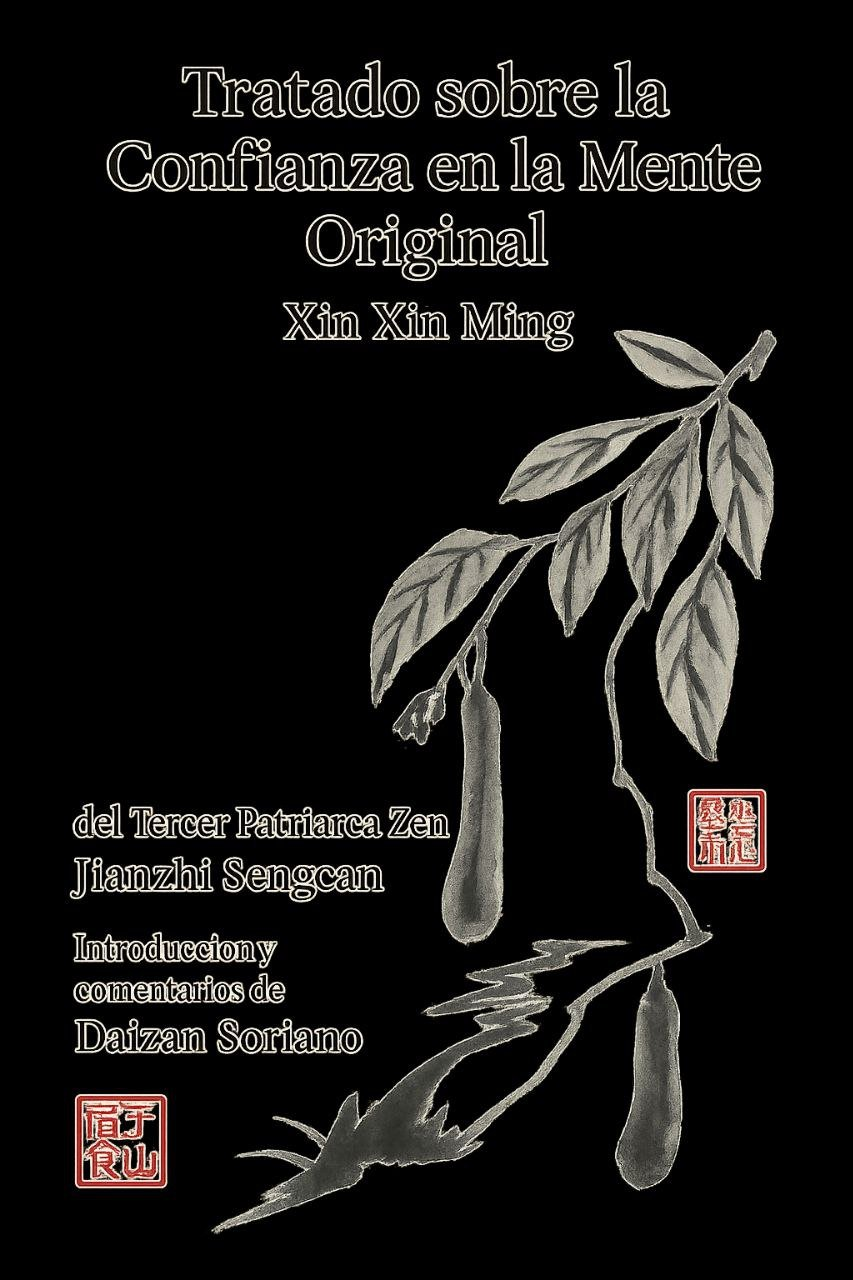
\includegraphics{../img/portada.jpg}

\textbf{Autor:} Daizan Soriano

\textbf{Primera edición:} 2025

Este libro está publicado bajo una licencia
\href{https://creativecommons.org/licenses/by-nc-sa/4.0/deed.es}{Creative
Commons Atribución-NoComercial-CompartirIgual 4.0 Internacional (CC
BY-NC-SA 4.0)} .


\includegraphics{../img/88x31.png}

Se permite copiar, distribuir y comunicar públicamente este material,
así como crear obras derivadas, siempre que se reconozca debidamente la
autoría, no se utilice para fines comerciales y se comparta bajo la
misma licencia.

Las imágenes utilizadas en este libro son de dominio público. Por
ejemplo: \emph{Japanese frog (late 18th-19th century)}, tinta y color
sobre papel por Getsuju. Imagen original de dominio público del
\href{https://collections.artsmia.org/}{Minneapolis Institute of Art},
mejorada digitalmente por rawpixel. Disponible para uso personal y
comercial.

Este libro ha sido desarrollado con el apoyo de la \textbf{Comunidad
Soto Zen Camino Medio (CSZCM)}, dedicada a la difusión de las enseñanzas
del Dharma y la práctica del Zen.

\href{https://www.caminomedio.org}{www.caminomedio.org}.

Versión 0.0.2

\textbf{© Daizan Soriano, 2025.}

\hfill\break

\newpage

\begin{center}\textbf{Introducción del autor}\end{center}

Este libro nace del deseo de acercar uno de los textos más esenciales de
la tradición Chan ---el \emph{Xin Xin Ming}, el \emph{Tratado sobre la
Confianza en la Naturaleza Original}--- a quienes buscan vivir la
práctica del Zen de manera sencilla, directa y profunda.

No escribo estas palabras como un erudito, ni como un experto. Escribo
como un compañero de camino y con el deseo de mantener viva la llama de
la transmisión recibida a través de mi maestro Dokushô Villalba roshi, y
de todos los maestros y maestras de nuestra tradición. Mi intención no
ha sido ofrecer una interpretación académica ni exhaustiva, sino una
lectura vivida, que pueda resonar en la experiencia cotidiana de quien
se acerque a estas páginas con el corazón abierto.

El \emph{Xin Xin Ming} ha sido una presencia constante en mi vida desde
que empecé a estudiarlo hace cinco años. He estudiado el texto basándome
en la traducción y comentarios de Taisen Deshimaru roshi ---maestro de
mi maestro--- publicada bajo el título \emph{Poema de la Fe en el
Espíritu}, enraizada a su vez en las enseñanzas de Kodo Sawaki y los
comentarios de Keizan Jokin. También me he apoyado en la traducción
directa del chino realizada por Dokushô Villalba roshi, recogida en su
libro \emph{Canto al Corazón de la Confianza}, cuya claridad y
profundidad han sido una guía indispensable.

En este libro, cada verso y su comentario han sido escritos de forma
independiente, de modo que se pueda abrir por cualquier página y
encontrar en cada lectura un espejo vivo que dialogue con la experiencia
personal de cada momento. No es necesario seguir un orden lineal: cada
verso es una puerta abierta a la confianza en la naturaleza original.

Las siguientes palabras de Dôgen Zenji, en el \emph{Shôbôgenzô
Zuimonki}, me han alentado para compartir mis reflexiones en este libro:

\emph{No hace falta escribir poesía para expresar lo que se siente con
el corazón. No hace falta ser un literato para escribir sobre el Dharma.
Si queréis escribir textos sobre el Dharma, no tratéis de escribir de
acuerdo con las reglas de la literatura ni de la retórica, no penséis en
las rimas ni en ningún otro fenómeno lingüístico. Dejad que el lenguaje
y el estilo se desarrollen por ellos mismos. Lo único importante es
escribir detalladamente la verdad que queréis expresar.}

Este trabajo recoge las reflexiones que empecé a compartir en la
primavera de 2021 a través de mi página web
\href{https://daizansoriano.com}{daizansoriano.com}, ahora reunidas aquí
con el propósito de ponerlas al servicio de los practicantes de la
Comunidad Soto Zen Camino Medio (CSZCM) y de todas las personas
interesadas en el budismo Soto Zen.

Como acompañamiento a este libro, he desarrollado también un
temporizador de meditación disponible en la página
\href{https://www.caminomedio.org}{www.caminomedio.org}, que ofrece, al
finalizar cada sesión de zazen, un verso del \emph{Xin Xin Ming} junto a
su comentario como inspiración para la práctica cotidiana.

Que este trabajo sea para el bien de todos los seres.

\textbf{Daizan Soriano}\\
Primavera de 2021 -- Primavera de 2025

\newpage

\begin{center}\textbf{Introducción al Xin Xin Ming}\end{center}

El \emph{Xin Xin Ming} (信心銘), que traduzco en esta versión como
\emph{Tratado sobre la Confianza en la Naturaleza Original}, es uno de
los textos más antiguos y significativos dentro de la tradición del
budismo Chan (Zen en japonés). Atribuido tradicionalmente al Tercer
Patriarca Chan, el maestro Jianzhi Sengcan (Kanchi Sōsan en japonés),
este poema breve pero inmensamente profundo condensa la esencia del
despertar en un lenguaje sencillo y directo, libre de las elaboradas
construcciones filosóficas que caracterizaban otras corrientes budistas
de su época.

La fuerza del \emph{Xin Xin Ming} reside en su capacidad de señalar
directamente la no-dualidad de la existencia, la unidad intrínseca entre
mente y fenómenos, entre quien percibe y lo percibido. No se trata de un
texto para ser analizado intelectualmente, sino para ser leído,
asimilado y vivido desde la experiencia directa.

\hypertarget{contexto-histuxf3rico}{%
\subsection{Contexto histórico}\label{contexto-histuxf3rico}}

Jianzhi Sengcan vivió en una época de gran agitación en China, marcada
por persecuciones religiosas y cambios políticos. Aunque los datos
históricos sobre su vida son escasos, la tradición sostiene que fue
discípulo de Dazu Huike, el Segundo Patriarca Chan, y que recibió la
transmisión del Dharma en circunstancias difíciles, en un clima donde el
budismo era objeto de restricciones y censura.

Su enseñanza destaca por su simplicidad y su enfoque en la confianza
profunda en la naturaleza original de la mente, sin apoyarse en rituales
o doctrinas complejas. Sengcan encarna así la esencia de la enseñanza
Chan: soltar los apegos intelectuales y confiar plenamente en la
sabiduría que ya está presente en cada uno de nosotros/as.

\hypertarget{significado-del-tuxedtulo}{%
\subsection{Significado del título}\label{significado-del-tuxedtulo}}

El título del poema puede entenderse como una declaración o canto acerca
de la confianza incondicional en la mente original:

\begin{itemize}
\tightlist
\item
  \textbf{Xin (信)}: significa fe, confianza o convicción, no en un
  sentido de creencia ciega, sino como una profunda seguridad basada en
  la experiencia.
\item
  \textbf{Xin (心)}: alude al corazón y a la mente como una única
  realidad, que en la tradición Chan se concibe como no-dual y no
  fragmentada.
\item
  \textbf{Ming (銘)}: hace referencia a una inscripción o tratado
  solemne, indicando que el contenido del texto está destinado a ser
  recordado y contemplado.
\end{itemize}

Así, el \emph{Xin Xin Ming} podría interpretarse como un recordatorio
perenne de la confianza en la verdadera naturaleza de nuestra
existencia.

\hypertarget{temas-principales-del-xin-xin-muxedng}{%
\subsection{\texorpdfstring{Temas principales del \emph{Xin Xin
Míng}}{Temas principales del Xin Xin Míng}}\label{temas-principales-del-xin-xin-muxedng}}

\begin{itemize}
\tightlist
\item
  \textbf{La no-dualidad}: Se supera la visión dualista que separa
  sujeto y objeto, bien y mal, vida y muerte. Todo es visto como una
  manifestación inseparable del mismo principio.
\item
  \textbf{La confianza en la naturaleza de la mente}: El despertar no se
  encuentra fuera de nosotros/as; es la confianza en la mente tal como
  es, sin añadidos, sin modificaciones.
\item
  \textbf{La ausencia de esfuerzo}: El poema enseña que la iluminación
  no es una meta a alcanzar con esfuerzo, sino el resultado natural de
  dejar de buscar y descansar en la realidad tal como es.
\end{itemize}

\hypertarget{la-relaciuxf3n-con-el-taouxedsmo}{%
\subsection{La relación con el
taoísmo}\label{la-relaciuxf3n-con-el-taouxedsmo}}

La profunda influencia del taoísmo filosófico en el \emph{Xin Xin Ming}
es evidente en su lenguaje y enfoque. Ambas tradiciones comparten la
valoración de la espontaneidad, el desapego de los conceptos dualistas,
y el reconocimiento del \emph{Wu Wei} (無為) ---la acción sin esfuerzo
artificioso--- como un modo de vida en armonía con el flujo natural de
la existencia.

Entre los paralelismos con el \emph{Tao Te Ching} destacan:

\begin{itemize}
\tightlist
\item
  La fluidez y el no-apego: adaptarse a las circunstancias sin rigidez.
\item
  La trascendencia de las oposiciones: ir más allá de los pares de
  contrarios.
\item
  El valor del vacío: reconocer que el vacío no es carencia, sino
  plenitud abierta.
\item
  La simplicidad natural: vivir sin artificios, en sintonía con la
  naturaleza profunda de las cosas.
\end{itemize}

\hypertarget{influencia-y-legado}{%
\subsection{Influencia y legado}\label{influencia-y-legado}}

Desde sus orígenes, el \emph{Xin Xin Ming} ha sido una fuente de
inspiración tanto para maestros/as como para practicantes. Comentado y
transmitido de generación en generación, ha dejado una huella indeleble
en figuras clave del budismo zen como Keizan Jōkin, Dōgen Zenji y
numerosos maestros contemporáneos.

El poema sigue siendo un faro luminoso para quienes buscan una vía
directa hacia el despertar. Su lenguaje, despojado de artificios, sigue
tocando el corazón de la práctica, recordándonos que la naturaleza
original está siempre disponible aquí y ahora, y que el verdadero camino
consiste simplemente en confiar, soltar y ser.

\newpage

\begin{center}\textbf{Texto}\end{center}

\hypertarget{el-presente-texto-es-una-versiuxf3n-que-se-ajusta-a-la-esencia-del-xin-xin-ming-pero-con-un-estilo-muxe1s-libre-y-fluido-para-hacer-su-lectura-muxe1s-clara-y-accesible.-conserva-el-sentido-profundo-del-texto-original-pero-evita-construcciones-demasiado-cruxedpticas-permitiendo-que-su-mensaje-se-despliegue-de-manera-muxe1s-natural.-la-intenciuxf3n-es-que-cada-pasaje-resuene-con-la-experiencia-directa-del-lector-sin-necesidad-de-interpretaciones-complejas.}{%
\subparagraph{El presente texto es una versión que se ajusta a la
esencia del Xin Xin Ming, pero con un estilo más libre y fluido para
hacer su lectura más clara y accesible. Conserva el sentido profundo del
texto original, pero evita construcciones demasiado crípticas,
permitiendo que su mensaje se despliegue de manera más natural. La
intención es que cada pasaje resuene con la experiencia directa del
lector, sin necesidad de interpretaciones
complejas.}\label{el-presente-texto-es-una-versiuxf3n-que-se-ajusta-a-la-esencia-del-xin-xin-ming-pero-con-un-estilo-muxe1s-libre-y-fluido-para-hacer-su-lectura-muxe1s-clara-y-accesible.-conserva-el-sentido-profundo-del-texto-original-pero-evita-construcciones-demasiado-cruxedpticas-permitiendo-que-su-mensaje-se-despliegue-de-manera-muxe1s-natural.-la-intenciuxf3n-es-que-cada-pasaje-resuene-con-la-experiencia-directa-del-lector-sin-necesidad-de-interpretaciones-complejas.}}

\hfill\break

\hypertarget{tratado-sobre-la-confianza-en-la-naturaleza-original}{%
\subsection{Tratado sobre la Confianza en la Naturaleza
Original}\label{tratado-sobre-la-confianza-en-la-naturaleza-original}}

\hfill\break

La realización del Gran Despertar no es difícil. No requiere de
habilidades extraordinarias ni de un esfuerzo desmesurado, pero sí de
una actitud abierta y libre de fijaciones. Tan solo evita el apego y el
rechazo. Cuando la mente deja de dividir la realidad entre lo que desea
y lo que teme, surge de manera natural una comprensión clara y serena.

Cuando no aparece el apego ni el rechazo, todo manifiesta su naturaleza
luminosa. La vida se despliega en su plenitud cuando dejamos de
filtrarla a través del juicio. Si nos aferramos a una idea de cómo deben
ser las cosas, o si nos resistimos a lo que es, oscurecemos nuestra
percepción y nos desconectamos de la realidad.

Si aparece la más mínima diferencia, cielo y tierra quedan separados por
un abismo. La distinción artificial entre "yo" y "el mundo", entre
"bueno" y "malo", entre "correcto" e "incorrecto", es la raíz del
sufrimiento. Si deseas ver la verdad ante ti, no tomes partido a favor
ni en contra de nada. La sabiduría surge cuando dejamos de alimentar
nuestras preferencias y aversiones.

El conflicto entre lo que aceptas y lo que rechazas enferma el corazón y
la mente. La constante lucha interna por querer algo diferente a lo que
es, genera agotamiento y sufrimiento. Si no comprendes el principio
profundo, te esfuerzas en vano en buscar la quietud. La paz no es algo
que se pueda fabricar; solo se revela cuando dejamos de resistirnos a la
realidad tal cual es.

Pleno como el gran vacío, nada falta, nada sobra. La existencia es
completa en sí misma. No hay nada que deba añadirse ni eliminarse. Es
precisamente por aferrarnos y rechazar que perdemos nuestra armonía
natural. La mente crea sus propios obstáculos, dividiendo la realidad en
lo que le gusta y lo que no.

No persigas lo que surge de los fenómenos, ni te aferres a la vacuidad.
La verdadera libertad no está en renunciar al mundo ni en aferrarse a la
idea de un estado especial. Cultiva una mente y un corazón ecuánimes, y
la dualidad desaparecerá por sí misma. La ecuanimidad es la puerta a una
comprensión profunda que trasciende los opuestos.

Intentar detener el movimiento solo lo intensifica aún más. La rigidez
de querer controlar la mente solo genera más agitación. Cuando el
movimiento cesa, la calma regresa. La verdadera serenidad no se impone,
sino que surge cuando dejamos de luchar contra el flujo natural de la
existencia.

Aferrarse a los extremos impide realizar la unidad. La verdad no se
encuentra en los polos opuestos, sino en la totalidad que los abarca. Si
no alcanzas la unidad, te perderás en ambos extremos. La dualidad de
"correcto" e "incorrecto", "ser" y "no-ser", nos atrapa en una visión
limitada.

Al rechazar la existencia, se pierde su verdadera naturaleza; al
aferrarse al vacío, se niega su auténtico significado. Si te inclinas
demasiado hacia uno u otro lado, te desvías del Camino. Cuantas más
palabras y pensamientos, más lejos estamos de nuestra armonía
intrínseca. No es a través de la especulación intelectual que se alcanza
la comprensión, sino mediante la experiencia directa.

Cuando cesan las palabras y el sobrepensamiento, no hay lugar donde no
haya claridad. La mente en su estado natural es luminosa y clara, pero
el exceso de conceptos y análisis la oscurece. Volver al origen es
alcanzar la esencia; seguir las apariencias es alejarse de la
realización. Si diriges tu atención hacia la fuente de tu propia mente,
descubrirás lo que siempre ha estado presente.

Cuando la luz se dirige hacia el interior, en un instante se trasciende
el vacío ilusorio. Dejar de buscar afuera y volverse hacia la propia
experiencia permite ver más allá de las apariencias. Los cambios que
parecen tener lugar en el vacío surgen de una percepción equivocada
creada por la ignorancia. La realidad no está separada de ti, pero tu
forma de percibirla oscurece su naturaleza.

No necesitas buscar la verdad, tan solo suelta las percepciones
erróneas. La verdad no es algo que se alcanza, sino algo que se revela
cuando dejamos de aferrarnos a nuestras distorsiones. No te aferres a
puntos de vista dualistas, actúa con cuidado y no los persigas. La
visión de la realidad se aclara cuando soltamos la necesidad de
definirlo todo en términos opuestos.

Apenas surge el juicio de correcto e incorrecto, mente y corazón se
pierden en la confusión. La división constante entre lo que creemos que
debería ser y lo que es nos desconecta de la vida real. Aunque la
dualidad surge de la unidad, tampoco te aferres a la unidad. No
conviertas la unidad en un concepto más, pues entonces se vuelve una
trampa.

Cuando la mente no construye, los diez mil fenómenos se manifiestan sin
error. Todo está en su lugar cuando la mente no impone sus juicios. Sin
la noción de error, los fenómenos simplemente son. Sin construcciones
mentales, no hay apego ni rechazo. La ecuanimidad no es indiferencia,
sino ver las cosas sin distorsión, tal como son.

La existencia y la no-existencia dependen una de la otra, y sin embargo,
trascienden esta aparente contradicción. Lo infinitamente pequeño es
idéntico a lo infinitamente grande; cuando se olvidan los límites y se
disuelven las fronteras, la realidad se muestra tal cual es.

El ser es, en sí mismo, no-ser. El no-ser es, en sí mismo, ser. Estas no
son ideas abstractas, sino realidades que se pueden experimentar
directamente cuando la mente deja de aferrarse a sus propias
construcciones.

Uno es todo, todo es uno. Si comprendes esto, no hay motivo para
inquietarse. No hay nada que alcanzar porque nada falta. La esencia de
la confianza es la no-dualidad; la no-dualidad es la esencia de la
confianza.

Cuando cesa la búsqueda, el Camino se muestra con claridad. Cuando la
mente está libre de fijaciones, la realidad se despliega en su plenitud.
Una vez aquí, el lenguaje se silencia, y el pasado, el futuro y el
presente desaparecen. En ese instante, solo queda el fluir natural de la
existencia, sin nada que añadir ni que quitar.

\newpage

\begin{center}\textbf{}\end{center}

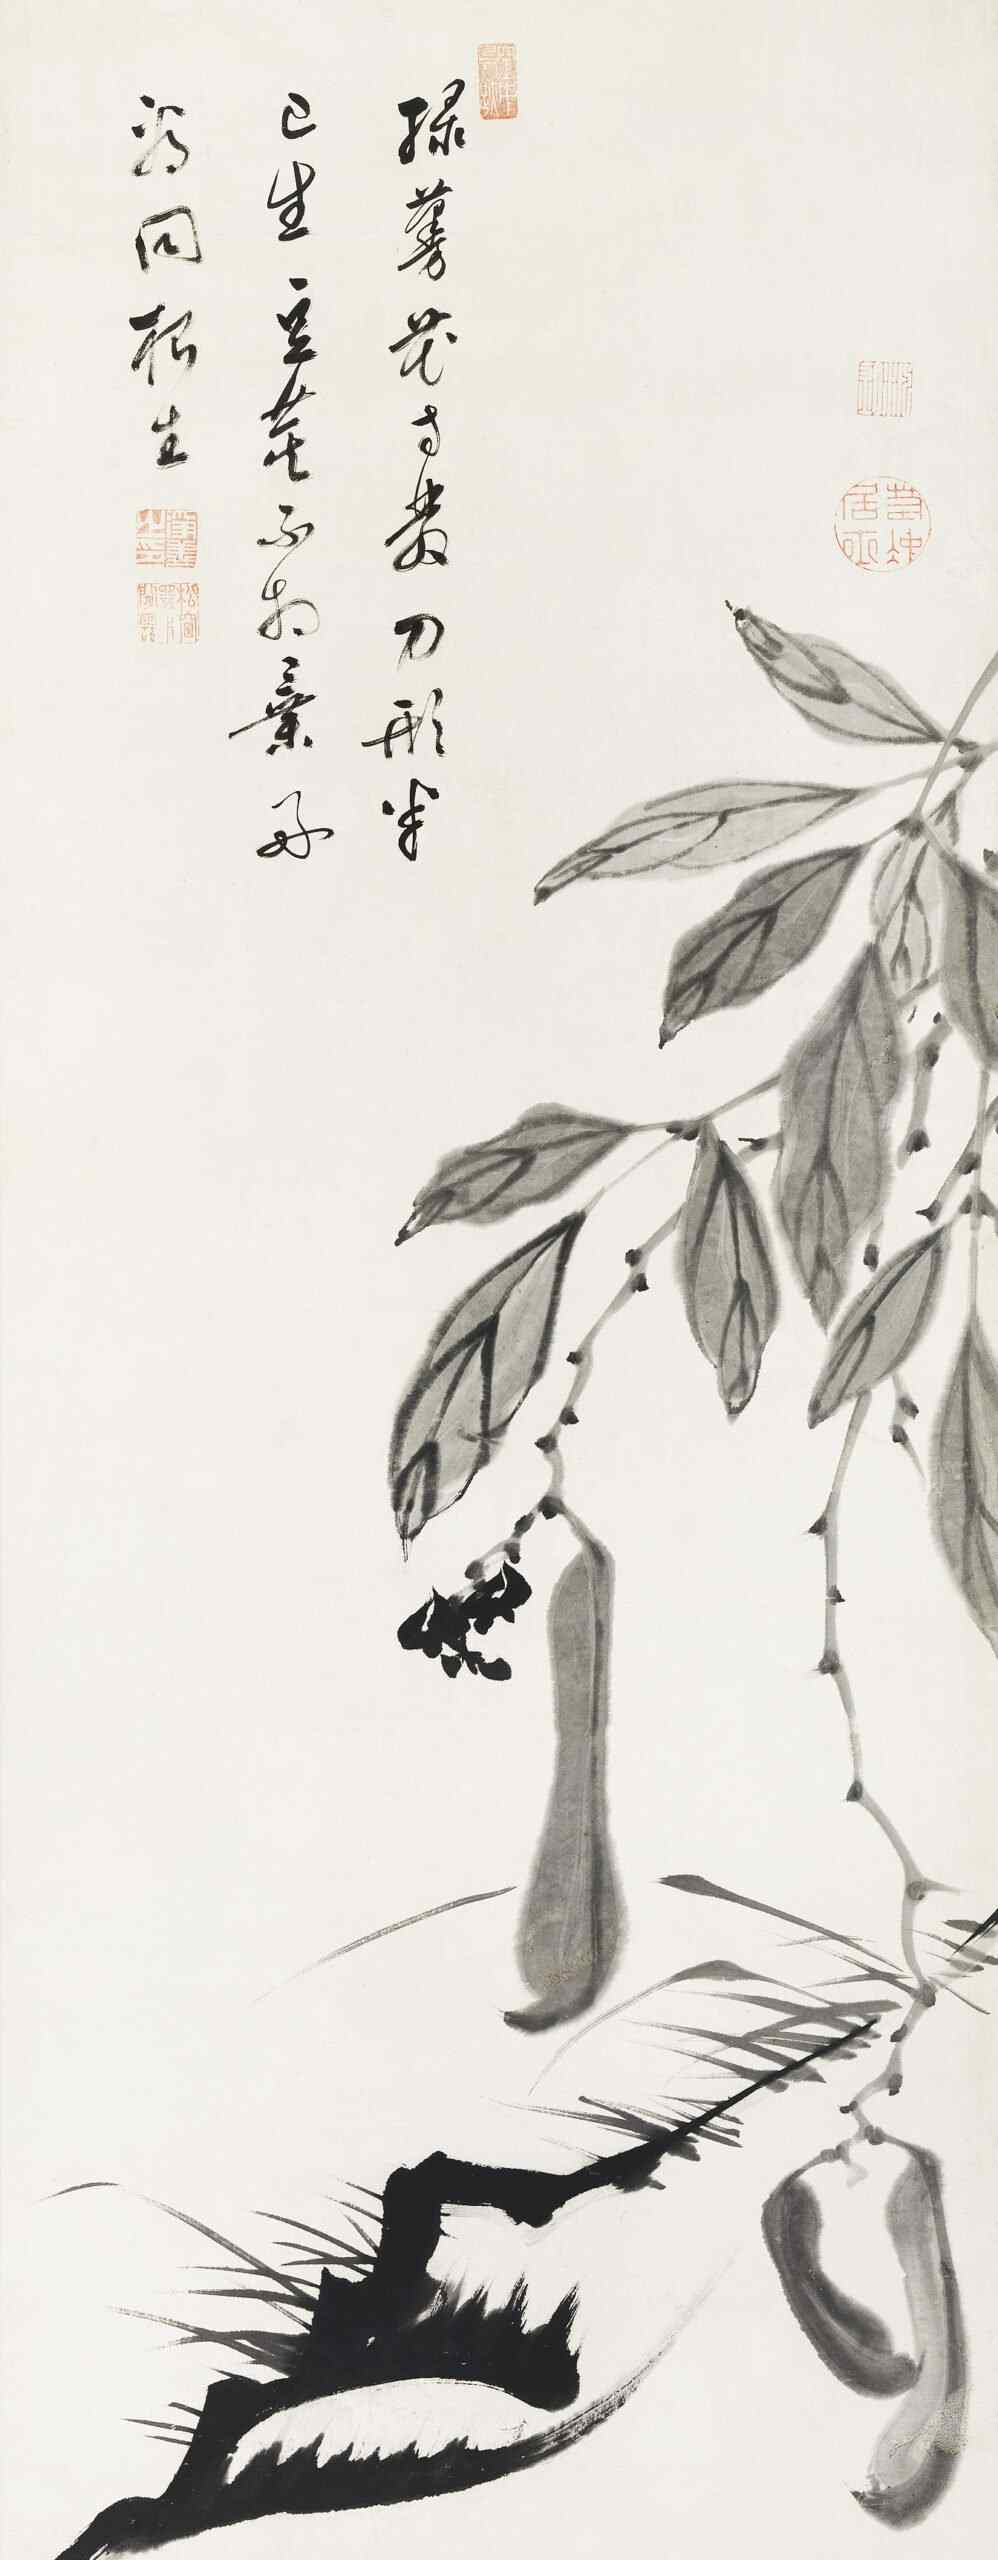
\includegraphics{../img/image01.jpg}

\begin{verseblock}

\newpage

\begin{center}\textbf{1.}\end{center}

至 道 無 難 唯 嫌 揀 擇

Zhì dào wù nán Wéi xián jiăn zé

La realización del Gran Despertar no es difícil,\\
tan solo evita el apego y el rechazo.

\end{verseblock}

\hypertarget{comentario}{%
\subsection{Comentario}\label{comentario}}

¿Qué es el Gran Despertar? El maestro Dôgen Zenji escribió: «Los ojos
son horizontales, la nariz vertical». Aquí y ahora, justo bajo tus pies
lo tienes disponible. Para acceder tan solo tienes que desprenderte del
yo y lo mío, shin jin datsu
raku\textsuperscript{\protect\hypertarget{ref1}{\protect\hyperlink{nota1}{1}}}.
, en palabras de Dôgen Zenji. Necesitamos desprendernos de nuestra
percepción ilusoria y aprender a percibir más allá de todo
condicionamiento, más allá de los conceptos y de las palabras con las
que describimos y recreamos el mundo instante tras instante.

¿Cómo acceder a esta percepción no condicionada por los constructos
mentales? El segundo verso no deja lugar a dudas, ``Tan solo evita el
apego y el rechazo''. Si me observo atentamente tomo conciencia de que
el movimiento interno de atracción y rechazo se produce automáticamente.
Rechazo lo que juzgo desagradable y me apego a lo que considero
agradable. Se puede manifestar en un diálogo interno del tipo: «Tengo
sobrepeso\ldots, Qué comida tan apetitosa\ldots, Soy un ignorante\ldots,
tengo que leer más\ldots».

Nos perdemos fácilmente en un mar de elecciones, tomando partido
continuamente, inconscientemente, con el piloto automático en marcha,
dirigido por nuestros condicionamientos socioculturales y personales.
¿Cómo salir de este círculo vicioso? En primer lugar, siendo consciente
de ello, aplicando la atención adecuada. Como dijo Ortega Y Gasset «No
sabemos lo que nos pasa y eso es precisamente lo que nos pasa.» O como
suele parafrasear el maestro Dokushô Villalba «lo que nos pasa es que no
sabemos lo que nos pasa, por eso nos pasa lo que nos pasa\ldots». Tomar
conciencia de qué es lo que está pasando nos conduce hacia la percepción
de las cosas tal cual son, más allá de nuestra visión ilusoria habitual.

La Realidad es lo que es, más allá de que nos resulte agradable o
desagradable. Las cosas son lo que son, pero las palabras y conceptos
nos hacen vivir en un espejismo continuo. Esta Realidad no la podemos
atrapar con la mente, con las palabras, con las ideas. Solo tendremos
acceso a ella, no tomando partido ni por ni contra. Esa actitud surge
naturalmente a través de la práctica correcta de zazen.

\hfill\break

\hypertarget{02}{}
\begin{verseblock}

\newpage

\begin{center}\textbf{2.}\end{center}

但 莫 憎 愛 洞 然 明 白

Dàn mò zēng ài dòng rán míng bái

Cuando no aparece el apego ni el rechazo,\\
todo manifiesta su naturaleza luminosa.

\end{verseblock}

\hfill\break

\hypertarget{comentario-1}{%
\subsection{Comentario}\label{comentario-1}}

Continuamente nos aferramos a lo que deseamos («apego»), y rechazamos lo
que nos resulta desagradable sin ser conscientes de ello. Nuestra
práctica consiste en observar, acechar y ver directamente cómo se
manifiesta esta atracción y rechazo en nuestra práctica y en nuestra
vida cotidiana, en qué forma y detalles concretos, en nuestras
circunstancias vitales.

La práctica de la atención plena nos permite observar este proceso con
todo detalle y nos da la oportunidad de experimentar plenamente de qué
manera se expresa en nuestra existencia. Una vez observado, vivenciado e
integrado completamente, la naturaleza luminosa de todo lo que nos rodea
se hace evidente, como el paso de la pierna derecha sigue al de la
izquierda.

Gracias a la ecuanimidad que nos proporciona la práctica de zazen, la
polarización amor-odio, apego-rechazo y cualquier otra dicotomía se
disuelve. Desde este estado de apertura ecuánime podemos experimentar
las cosas tal cual son para que la naturaleza luminosa de la realidad
surja naturalmente. Para ello debemos adoptar una aptitud de apertura,
sin tomar partido ni por ni contra, aceptando incondicionalmente
cualquier contenido que esté surgiendo en nuestro campo de experiencia.

Como dijo el maestro Eihei Dogen:
\textsuperscript{\protect\hypertarget{ref2}{\protect\hyperlink{nota2}{2}}}

Tened abiertas las manos y toda la arena del desierto pasará por ellas.
Cerradlas y solo conseguiréis unos pocos granos de arena.

\hfill\break

\hypertarget{03}{}
\begin{verseblock}

\newpage

\begin{center}\textbf{3.}\end{center}

毫 釐 有 差 天 地 懸 隔

Háo lí yŏu chā tiān dì xuán gé

Si aparece la más mínima diferencia,\\
cielo y tierra quedan separados por un abismo.

\end{verseblock}

\hfill\break

\hypertarget{comentario-2}{%
\subsection{Comentario}\label{comentario-2}}

Un abismo es una «realidad inmaterial inmensa, insondable o
incomprensible»\textsuperscript{\protect\hypertarget{ref3}{\protect\hyperlink{nota3}{3}}}.
En el estado ordinario de percepción ilusoria no podemos ni imaginar el
despertar, ni siquiera podemos intuir qué puede haber al otro lado del
abismo, cualquier tipo de idea al respecto es una ilusión.

En el budismo distinguimos dos verdades, la de la realidad condicionada
y la incondicionada. Desde la verdad del despertar, es posible integrar
sin paradoja alguna estas dos verdades, pero desde la orilla de la
percepción dualista, un abismo nos separa de la experiencia de la
realidad incondicionada.

¿Cómo experimentar la verdad incondicionada? A través de la práctica
perseverante. El Buda nunca describió el nirvana, porque en cuanto lo
conceptualizas, en cuanto utilizas el lenguaje, eso ya no es. Todo
intento de comprensión a través de las estructuras del lenguaje nos
aleja de la experiencia del despertar.

La realidad es como es más allá de los conceptos y las ideas que nos
hacemos de ella. Cuando percibimos la realidad desde el intelecto,
estamos utilizando el lenguaje y, por tanto, «creamos \ldots{}
diferencias». Esto quiere decir que no podemos tratar de aprehender la
realidad a través de los conceptos, es inútil intentar atrapar con la
mente lo que está más allá de cualquier concepto. El Tao Te
King\textsuperscript{\protect\hypertarget{ref4}{\protect\hyperlink{nota4}{4}}}
empieza con la frase «El Tao que puede ser expresado no es el verdadero
Tao». La realidad es no-dos, indivisible. El budismo
Mahayana\textsuperscript{\protect\hypertarget{ref5}{\protect\hyperlink{nota4}{5}}}
afirma que samsara y nirvana son no dos, esta realidad tal cual es, ya
es el nirvana, pero solo la mente que ha realizado el despertar puede
comprenderlo más allá de toda conceptualización.

\hfill\break

\hypertarget{04}{}
\begin{verseblock}

\newpage

\begin{center}\textbf{4.}\end{center}

欲 得 現 前 莫 存 順 逆

Yù dé xiàn qián, mò cún shùn nì.

Si deseas ver la verdad ante ti,\\
no tomes partido a favor ni en contra de nada.

\end{verseblock}

\hfill\break

\hypertarget{comentario-3}{%
\subsection{Comentario}\label{comentario-3}}

La mente sin cultivar se asemeja a un jardín descuidado, lleno de malas
hierbas o a un mono, saltando de un lado a otro sin parar, discriminando
de manera continua y automática, atrapada entre del apego, el rechazo y
la indiferencia a lo que valoramos como agradable, desagradable o
neutro. Esta situación nos impide ver la realidad tal cual es, más allá
de nuestra mente condicionada.

Durante zazen, nuestra actitud debe ser similar a la de alguien sentado
a la orilla de un río, dejando que el agua fluya sin intentar retener
nada, sin tomar partido ni a favor ni en contra. La vida es fluidez;
aferrarse o rechazar nos sumerge en un estado de guerra interna que nos
causa un sufrimiento ilusorio e innecesario. En la Vía del Buda evitamos
tomar partido a favor o contra absolutamente nada durante la meditación
sedente. Esta actitud permite que la sabiduría de nuestra naturaleza de
buda se manifieste naturalmente, sin obstáculo.

Para que la Totalidad se manifieste ante los ojos de la intuición, es
necesario ir más allá de nuestra mente discursiva ordinaria y cultivar
una actitud de aceptación y apertura incondicional.

En la tradición Zen decimos:

«Si te gusta, las cosas son como son; si no te gusta, las cosas son como
son».

Cultivar una aceptación incondicional permite que gradualmente la Vía se
clarifique naturalmente.

\hfill\break

\hypertarget{05}{}
\begin{verseblock}

\newpage

\begin{center}\textbf{5.}\end{center}

違 順 相 爭 是 爲 心 病

Wéi shùn xiāng zhēng, shì wèi xīn bìng

El conflicto entre lo que aceptas y lo que rechazas,\\
enferma el corazón y la mente.

\end{verseblock}

\hfill\break

\hypertarget{comentario-4}{%
\subsection{Comentario}\label{comentario-4}}

Cuando nos sentimos divididos, inmersos en un conflicto interno continuo
de tomar partido por o contra, experimentamos un desgaste gradual que
desemboca en la enfermedad del corazón y la mente. Esta enfermedad es
una manifestación de la falta de conexión con nuestra autenticidad más
profunda. En esta lucha perpetua entre los opuestos, perdemos el
contacto con nuestra verdadera naturaleza original, lo cual nos hace
caer en un estado interno de carencia continuo, algo nos falta y no
sabemos lo que es.

¿Cuál es el camino hacia la sanación de este estado? La respuesta reside
en reconectar con nuestra auténtica naturaleza original, donde la
bondad, la compasión, la alegría y la ecuanimidad se manifiestan de
manera natural. Cuando depositamos nuestra confianza serena en la
práctica de la Vía, nuestra vida cotidiana se impregna de esta sabiduría
innata. Para ello, la actitud adecuada es abstenernos de tomar partido
entre los opuestos, cesar de emitir juicios, y simplemente observar como
un espejo impecable refleja todo lo que se manifiesta ante él, sin
rechazar ni siquiera el apego y el rechazo.

Cuando tomamos conciencia de esta lucha entre los opuestos, cesamos en
ella, dejamos de alimentar la enfermedad, y la sanación surge de forma
espontánea, sin la necesidad de ninguna intención por nuestra parte.
Regresamos al estado de equilibrio, plenamente conscientes y despiertos.

\hfill\break

\begin{center}\rule{0.5\linewidth}{0.5pt}\end{center}

\leavevmode\vadjust pre{\hypertarget{notas}{}}%
\textsuperscript{1} Expresión que se suele traducir por «abandono de
cuerpo y mente» a través de ella el maestro Dôgen Zenji realizó la Vía
\protect\hyperlink{ref1}{Volver}

\textsuperscript{2} Eihei Dōgen (永平道元) también Dōgen Zenji
(道元禅師) o Dōgen Kigen (道元希玄) o Koso Joyo Daishi (literalmente
Ancestro Eminente, Sustentador de Luz, Gran Maestro) (Kioto, 26 de enero
de 1200 -- Ib., 29 de septiembre de 1253) fue el maestro zen fundador de
la escuela Sōtō del Zen en Japón. \protect\hyperlink{ref2}{Volver}

\textsuperscript{3} \href{https://dle.rae.es/abismo?m=form}{según la
RAE.} \protect\hyperlink{ref3}{Volver}

\textsuperscript{4}
\href{https://es.wikipedia.org/wiki/D\%C3\%A0od\%C3\%A9_j\%C4\%ABng}{El
Dàodé jīng} (Chino: 道德經 pronunciaciónⓘ, Wade-Giles: Tao Te Ching,
también llamado Tao Te King), también llamado Laozi (老子), es un texto
clásico chino atribuido al sabio Lao-Tse del siglo VI a. C., aunque su
fecha y autoría están abiertas al debate, es un texto clásico chino.
\protect\hyperlink{ref4}{Volver}

\textsuperscript{5}
\href{https://es.wikipedia.org/wiki/Mah\%C4\%81y\%C4\%81na}{Mahāyāna}
(sánscrito: «Gran Vehículo», o Bodhisattvayāna, «Vehículo del
Bodhisattva»)1\hspace{0pt} es, junto con el Theravada, una de las dos
ramas principales del budismo y un término para la clasificación de las
filosofías y prácticas budistas. Este movimiento acepta un gran número
de otros textos (sutras Mahāyāna) y doctrinas.
\protect\hyperlink{ref5}{Volver}

\hfill\break

\hfill\break

\hypertarget{01}{}
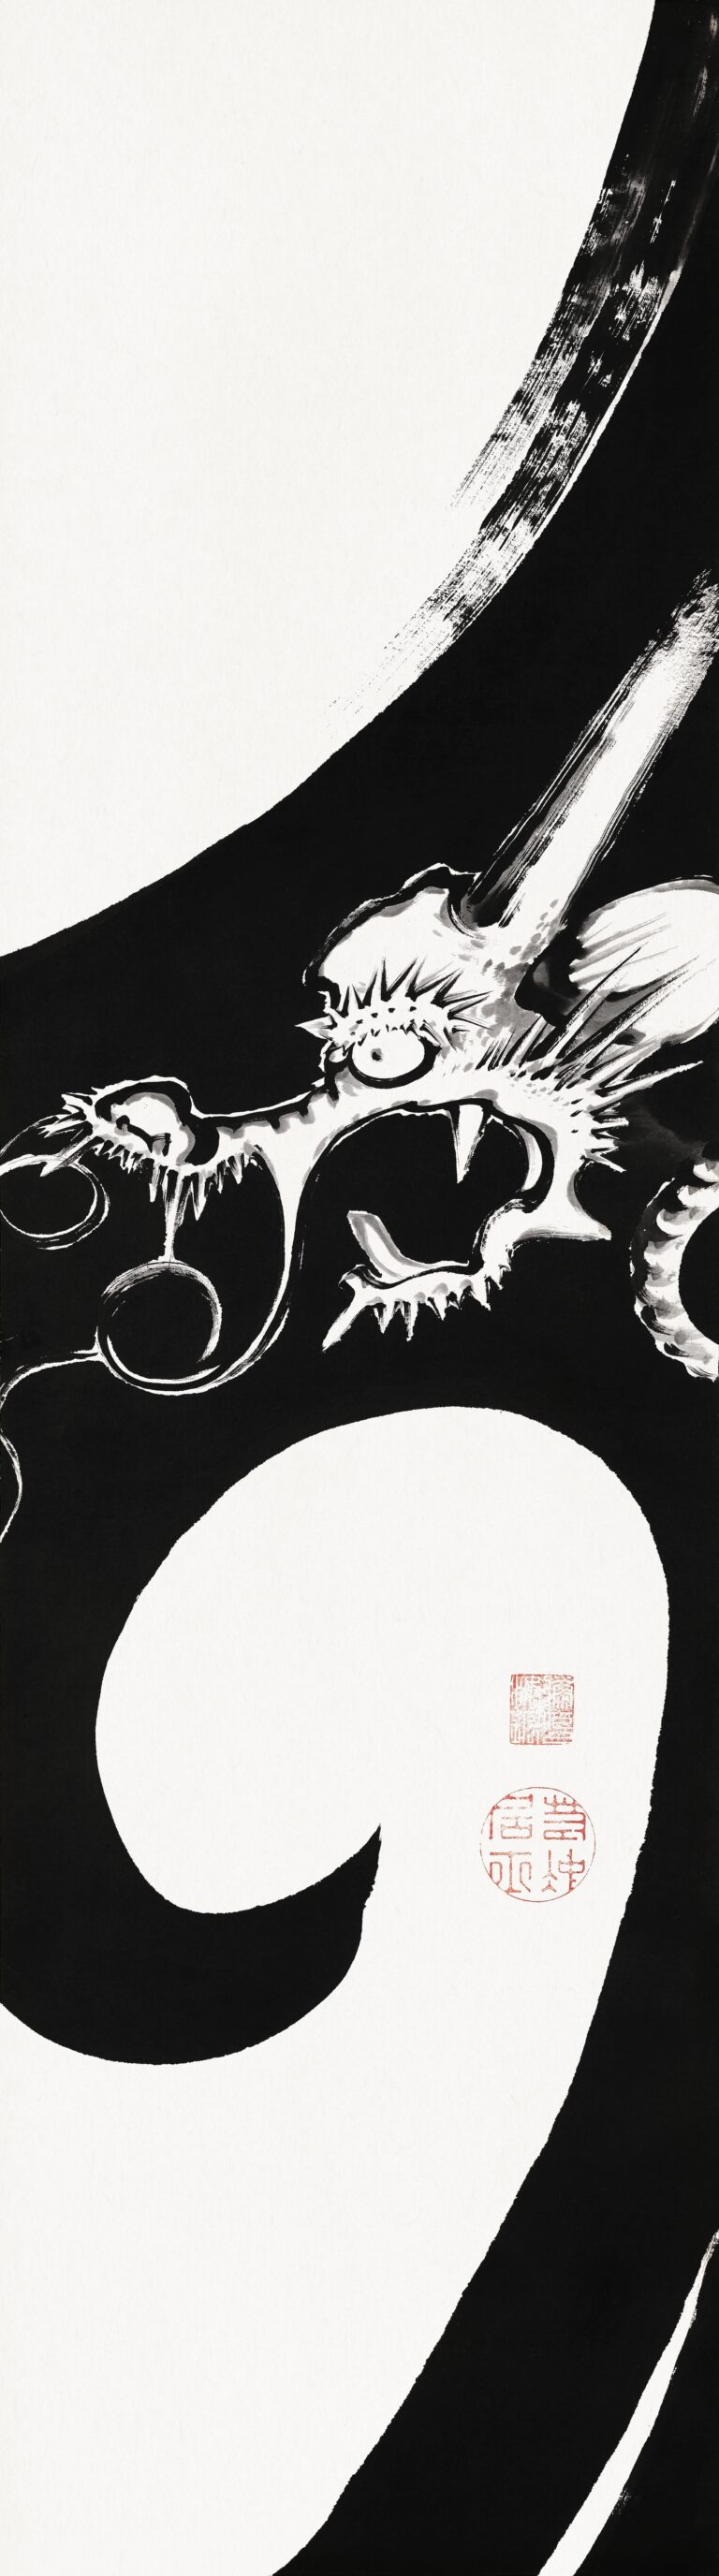
\includegraphics{../img/image02.jpg}

\begin{verseblock}

\newpage

\begin{center}\textbf{6.}\end{center}

不 識 玄 旨 徒 勞 念 靜

Bù shí xuán zhĭ tú láo niàn jìng

Si no comprendes el principio profundo,\\
te esfuerzas en vano en buscar la quietud.

\end{verseblock}

\hfill\break

\hypertarget{comentario-5}{%
\subsection{Comentario}\label{comentario-5}}

¿Cómo comprender el sentido profundo? ¿Leyendo y estudiando? Hasta
cierto punto es necesario el estudio intelectual, pero solo podemos
llegar a la sabiduría profunda mediante la experiencia directa. Es
inútil intentar comprender solo desde el intelecto. Leer y estudiar la
sabiduría que nos han legado nuestros ancestros es fundamental, a través
de ella podemos desarrollar la intuición. Pero esto no deja de ser como
el dedo que señala la luna, debemos cuidar de no quedarnos mirando el
dedo olvidándonos de experimentar la luna. Tenemos que recorrer el
camino poniendo en práctica nuestra comprensión y comprendiendo nuestras
experiencias.

No ver la realidad tal cual es, perturba nuestro estado natural que es
la paz serena del corazón. Continuamente nos enredamos en el caos que
causa nuestra ignorancia, nuestra ceguera, nuestra incapacidad de ver
con claridad. Lo constatamos, por ejemplo, en los continuos conflictos
que surgen en nuestras relaciones interpersonales. Somos como un
elefante entrando en una cacharrería, reaccionando impulsivamente ante
cualquier estímulo que juzgamos como intolerable o inadecuado.

¿Tu corazón está cada vez más sereno? Es el mejor indicador de que tus
pasos en la Vía van en la dirección adecuada. A través de la práctica
correcta y continuada de zazen nos vamos armonizando con el despertar a
la realidad tal cual es, naturalmente, día a día y conectando cada vez
más profundamente con la imperturbable serenidad del corazón.

\hfill\break

\hypertarget{02}{}
\begin{verseblock}

\newpage

\begin{center}\textbf{7.}\end{center}

圓 同 太 虚 無 欠 無 餘

Yuán tóng tài xŭ wú qiàn, wú yú

Plena como el gran vacío,\\
nada falta, nada sobra.

\end{verseblock}

\hfill\break

\hypertarget{comentario-6}{%
\subsection{Comentario}\label{comentario-6}}

Es nuestra incapacidad de aceptarnos plenamente, de abrirnos, la que nos
crea una insatisfacción profunda. Cuando se realiza la realidad tal cual
es, todo es ya perfecto. Todo ocupa su exacto lugar porque si algo
faltara o sobrara, dado que todo está interconectado, todo por completo
cambiaría y no sería tal cual es. ¿Qué sentido tiene, pues, desear o
rechazar? Lo único que obtendremos es más insatisfacción.

Juzgamos la realidad desde nuestra perspectiva limitada, por ejemplo,
señalando las injusticias, guerras y sufrimiento como imperfecciones.
Sin embargo, esta percepción es una visión fragmentada de la totalidad.
Desde la perspectiva de la Vía, incluso las situaciones difíciles tienen
su lugar y función. Esto no implica que debamos ser indiferentes ante el
sufrimiento, sino que nuestra acción debe surgir de un lugar de
comprensión y compasión, no desde el rechazo o la aversión.

Cuando comprendemos que ``nada falta, nada sobra'', nuestra motivación
para actuar no proviene del deseo de cambiar la realidad para ajustarla
a un ideal, sino de la compasión que surge de nuestra interconexión con
todo lo que existe. Esta comprensión nos permite soltar el anhelo y el
rechazo, viviendo en paz con la totalidad de lo que somos y de lo que
es, permitiendo que nuestra acción surja de la sabiduría y la compasión
fruto de nuestra práctica.

\hfill\break

\hypertarget{03}{}
\begin{verseblock}

\newpage

\begin{center}\textbf{8.}\end{center}

良 由 取 捨 所 以 不 如

Liáng yóu qŭ shě suŏ yĭ bù rú

Es precisamente por aferrarnos y rechazar,\\
que perdemos nuestra armonía natural.

\end{verseblock}

\hfill\break

\hypertarget{comentario-7}{%
\subsection{Comentario}\label{comentario-7}}

Un abismo es una «realidad inmaterial inmensa, insondable o
incomprensible»\textsuperscript{\protect\hypertarget{ref3}{\protect\hyperlink{nota3}{3}}}.
En el estado ordinario de percepción ilusoria no podemos ni imaginar el
despertar, ni siquiera podemos intuir qué puede haber al otro lado del
abismo, cualquier tipo de idea al respecto es una ilusión.

En el budismo distinguimos dos verdades, la de la realidad condicionada
y la incondicionada. Desde la verdad del despertar, es posible integrar
sin paradoja alguna estas dos verdades, pero desde la orilla de la
percepción dualista, un abismo nos separa de la experiencia de la
realidad incondicionada.

¿Cómo experimentar la verdad incondicionada? A través de la práctica
perseverante. El Buda nunca describió el nirvana, porque en cuanto lo
conceptualizas, en cuanto utilizas el lenguaje, eso ya no es. Todo
intento de comprensión a través de las estructuras del lenguaje nos
aleja de la experiencia del despertar.

La realidad es como es más allá de los conceptos y las ideas que nos
hacemos de ella. Cuando percibimos la realidad desde el intelecto,
estamos utilizando el lenguaje y, por tanto, «creamos \ldots{}
diferencias». Esto quiere decir que no podemos tratar de aprehender la
realidad a través de los conceptos, es inútil intentar atrapar con la
mente lo que está más allá de cualquier concepto. El Tao Te
King\textsuperscript{\protect\hypertarget{ref4}{\protect\hyperlink{nota4}{4}}}
empieza con la frase «El Tao que puede ser expresado no es el verdadero
Tao». La realidad es no-dos, indivisible. El budismo
Mahayana\textsuperscript{\protect\hypertarget{ref5}{\protect\hyperlink{nota4}{5}}}
afirma que samsara y nirvana son no dos, esta realidad tal cual es, ya
es el nirvana, pero solo la mente que ha realizado el despertar puede
comprenderlo más allá de toda conceptualización.

\hfill\break

\hypertarget{04}{}
\begin{verseblock}

\newpage

\begin{center}\textbf{9.}\end{center}

欲 得 現 前 莫 存 順 逆

Yù dé xiàn qián, mò cún shùn nì.

Si deseas ver la verdad ante ti,\\
no tomes partido a favor ni en contra de nada.

\end{verseblock}

\hfill\break

\hypertarget{comentario-8}{%
\subsection{Comentario}\label{comentario-8}}

En nuestra vida cotidiana, estamos inmersos en un flujo constante de
estímulos, eventos, emociones y pensamientos, lo que en budismo se llama
``fenómenos'' o ``dharmas''. Estos fenómenos son cambiantes,
transitorios y carecen de esencia fija. Sin embargo, la mente
condicionada tiende a aferrarse a ellos, a verlos como algo concreto y
estable. Este apego a los fenómenos provoca sufrimiento porque olvidamos
su naturaleza impermanente. Corremos detrás de ellos en un esfuerzo
inútil por encontrar seguridad o felicidad en lo que, por su misma
naturaleza, no puede ofrecernos estabilidad.

En el Sutra Corazón de la Gran
Sabiduría\textsuperscript{\protect\hypertarget{ref1}{\protect\hyperlink{nota1}{1}}}
recitamos cada día:

Shariputra, los fenómenos no son diferentes de
shûnyata\textsuperscript{\protect\hypertarget{ref2}{\protect\hyperlink{nota2}{2}}}.
Shûnyata no es diferente de los fenómenos. Los fenómenos son shûnyata.
Shûnyata es fenómenos.

Fenómeno y vacuidad forman parte de nuestra existencia y, sin embargo,
nuestros condicionamientos no nos permiten percibir el vacío,
generalmente solo somos capaces de percibir objetos independientes a los
que dotamos de entidad propia. Pero, no existe una separación real entre
lo que consideramos ``algo'' y el ``vacío''. Lo que percibimos como
fenómeno, lo que parece sólido y real, es en esencia vacío, carente de
un yo independiente, con existencia propia. El maestro zen Dogen expresó
esta verdad en su célebre frase "shin jin datsu raku", ``abandona,
cuerpo y
mente''\textsuperscript{\protect\hypertarget{ref3}{\protect\hyperlink{nota3}{3}}}.
La vacuidad y los fenómenos no están separados, son dos caras de la
misma moneda. No se trata de rechazar lo que vemos, sentimos o
experimentamos, sino de verlo tal como es: vacío de sustancia fija, pero
al mismo tiempo pleno en su manifestación.

No es suficiente con liberarse del apego a los fenómenos, sino que
también es necesario evitar el apego a la vacuidad. Vacuidad, no es la
``nada'' en sentido nihilista. Es el reconocimiento de que todas las
cosas carecen de una esencia fija y que dependen de causas y
condiciones. Pero cuando uno se apega a la vacuidad, se corre el riesgo
de caer en la trampa de la indiferencia, en el error de rechazar la
realidad fenoménica como algo insignificante o ilusorio.

Tenemos que situarnos más allá de los opuestos, la bóveda celeste
contiene las nubes y el espacio vacío entre ellas, tenemos que
trascender cualquier dicotomía y aprender a percibir la realidad desde
Mushotoku\textsuperscript{\protect\hypertarget{ref4}{\protect\hyperlink{nota4}{4}}},
nada que obtener, nada que aferrar. Cuando dejamos de buscar algo a lo
que aferrarnos, cuando dejamos de tratar de alcanzar o rechazar
cualquier cosa, nos situamos en la Vía. La percepción desde mushotoku es
libre de las trampas del deseo y del rechazo, y nos permite habitar la
realidad tal como es.

\hfill\break

\hypertarget{05}{}
\begin{verseblock}

\newpage

\begin{center}\textbf{10.}\end{center}

一 種 平 懷 泯 然 自 盡

Yī zhŏng ping huái mĭn rán zì jìn

Cultiva una mente y un corazón ecuánimes,\\
y la dualidad desaparecerá por sí misma.

\end{verseblock}

\hfill\break

\hypertarget{comentario-9}{%
\subsection{Comentario}\label{comentario-9}}

Cuando nos dejamos caer en la confianza serena del corazón, moramos
naturalmente en la serenidad del
samadhi\textsuperscript{\protect\hypertarget{ref5}{\protect\hyperlink{nota5}{5}}}.
Este es la actitud y el estado que cultivamos durante la práctica de
zazen3.

Pero, ¿cómo podemos trasladar esta serenidad a nuestra vida cotidiana,
inmersa en agitación, ansiedad y el estrés constante que nos arrastra?
Estos estados nos alejan por completo de nuestra naturaleza original, de
nuestra serenidad genuina. Para soportarlo, recurrimos automáticamente a
anestésicos temporales y distracciones efímeras que actúen como
sustitutos imperfectos de la verdadera calma.

Cuando nos sumergimos en la serenidad de la Unidad, la dualidad ---ese
constante vaivén entre lo correcto y lo incorrecto, el placer y el
dolor, el deseo y el rechazo--- comienza a disolverse de manera natural.
No es algo que necesitemos forzar; no hay una lucha consciente para
eliminar los opuestos. Simplemente, al descansar en la Unidad, la mente
deja de fragmentar la realidad en partes conflictivas. La dualidad
desaparece espontáneamente porque dejamos de aferrarnos a ella. En su
lugar, lo que surge es una percepción unificada, donde los aparentes
opuestos se integran en una totalidad más vasta.

Cultivar una mente y un corazón ecuánimes requiere encontrar y mantener
el equilibrio entre los opuestos. Es mediante la práctica del camino
medio, que trascendemos y abarcamos estos aparentes opuestos, logrando
de esta manera alcanzar un estado de equilibrio profundo.

Con el tiempo, al sumergirnos repetidamente en esta unidad serena, zazen
tras zazen, día tras día, comienza a surgir en nosotros una manera más
espontánea y natural de afrontar la vida cotidiana. Llevamos a cabo
nuestras actividades diarias como cualquier otro ser humano, pero con un
trasfondo de calma, lúcida y serena, que impregna todas nuestras
acciones. Este fondo silencioso de serenidad nos acompaña y sostiene,
ofreciéndonos un puerto seguro en medio de la vida cotidiana al cual
siempre podemos volver cuando la vida inevitablemente nos zarandee, ya
que, en realidad, nunca ha dejado de estar ahí.

\hfill\break

\begin{center}\rule{0.5\linewidth}{0.5pt}\end{center}

\leavevmode\vadjust pre{\hypertarget{notas}{}}%
\textsuperscript{1} Maha Prajña Paramita Hridaya Sutra, en sánscrito.
Maka Hannya Haramita Shingyo, en japonés.
\protect\hyperlink{ref1}{Volver}

\textsuperscript{2} Śūnyatā (AITS, /shuniáta/ o /shuniátaa/; Devanagari:
शून्यता; Pali: suññatā),1\hspace{0pt} a menudo traducido como
"vacuidad", "vaciedad" o "vació" es un concepto budista que tiene
múltiples significados dependiendo de su contexto doctrinal. Puede
referirse a una comprensión ontológica de la realidad, un estado
meditativo o un análisis fenomenológico de la experiencia.
\href{https://es.wikipedia.org/wiki/Shuniata}{Fuente.}
\protect\hyperlink{ref2}{Volver}

\textsuperscript{3} Un día en que Dogen estaba sentado en Zazen, su
vecino se durmió. El maestro Nyojo golpeo con fuerza al discípulo y con
voz fuerte gritó: ``¡Zazen es abandonar cuerpo y mente!: ¿Por qué
duermes?''. Al oír estas palabras, Dogen experimento el gran despertar.
Después Dogen fue a ver a Nyojo y le dijo:

``--- He abandonado cuerpo y mente -- shin jin datsu raku''.

Nyojo le contestó:

``-¡Abandona ahora la noción de haber abandonado cuerpo y mente!''

Dogen se postró entonces respetuosamente ante Nyojo y este añadió:
``Cuerpo y mente han sido abandonados -- datsu raku shin jin''
\protect\hyperlink{ref3}{Volver}

\textsuperscript{4} Mushotoku es una expresión zen (無所得) que podría
traducirse literalmente como `no provecho', `no obtención', o `nada que
obtener', lo que viene a significar `hacer algo sin esperar ningún
beneficio personal'. \protect\hyperlink{ref4}{Volver}

\textsuperscript{5} Mushotoku es una expresión zen (無所得) que podría
traducirse literalmente como `no provecho', `no obtención', o `nada que
obtener', lo que viene a significar `hacer algo sin esperar ningún
beneficio personal'. \protect\hyperlink{ref4}{Volver}

Estado de profunda concentración meditativa en el cual la mente se
vuelve completamente unificada y tranquila, dejando de estar dispersa o
distraída. En este estado, el sentido de separación entre el sujeto y el
objeto desaparece, y el practicante experimenta una absorción completa
en la experiencia presente, trascendiendo la dualidad.\\

\hfill\break

\hypertarget{01}{}
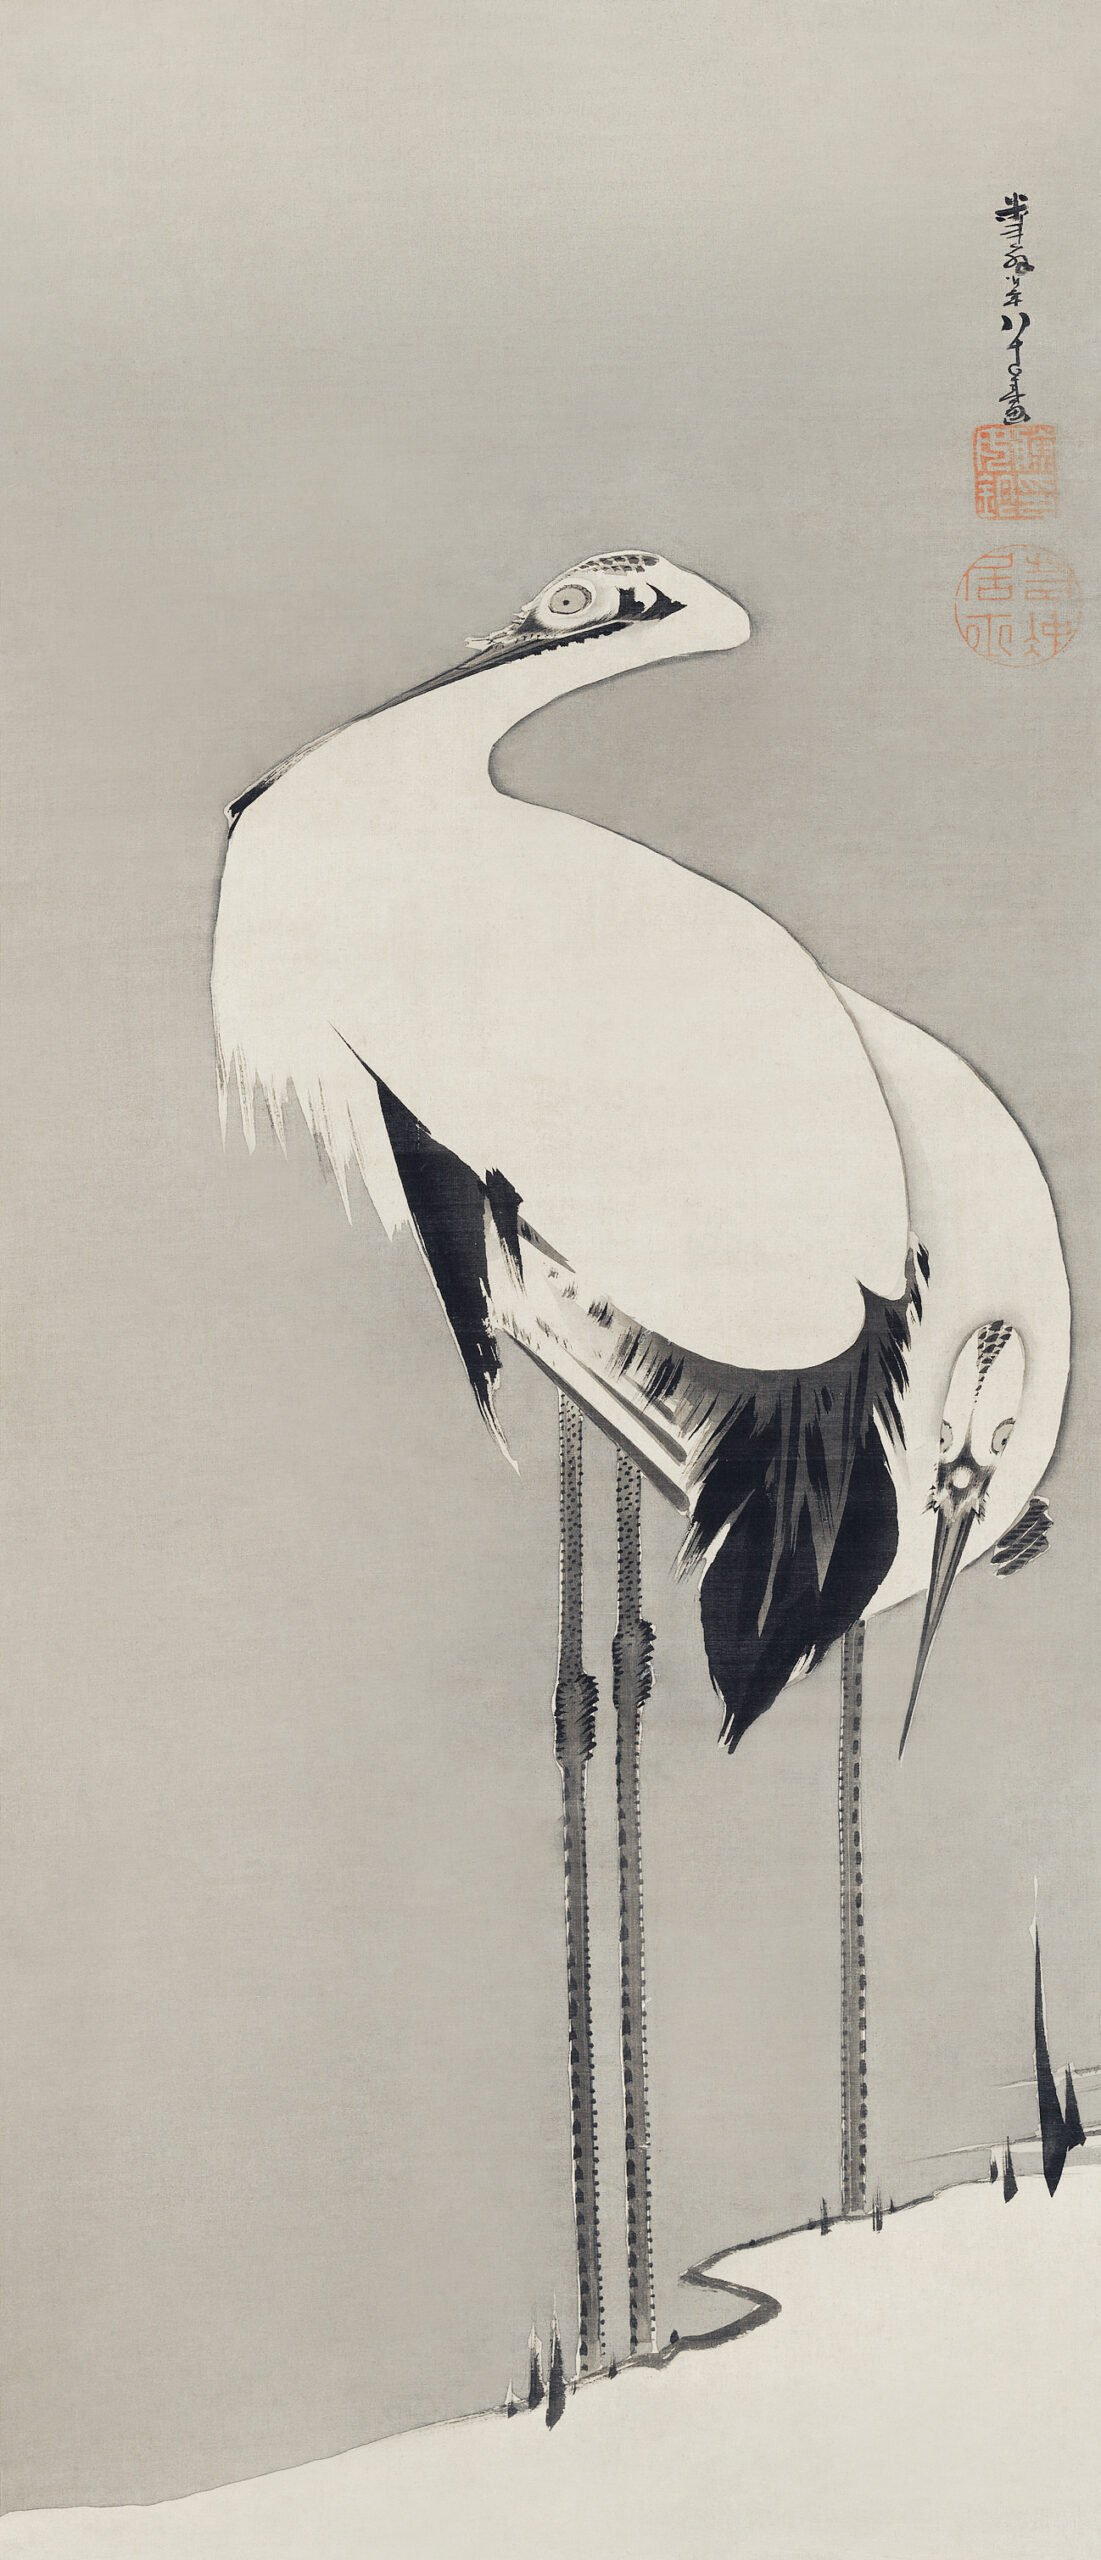
\includegraphics{../img/image03.jpg}

\begin{verseblock}

\hypertarget{section-12}{%
\subsection{11.}\label{section-12}}

止 動 歸 止 止 更 彌 動

Zhĭ dòng guī zhĭ zhĭ gèng mí dòng

Intentar detener el movimiento solo lo intensifica aún más,\\
cuando el movimiento cesa, la calma regresa.

\end{verseblock}

\hfill\break

\hypertarget{comentario-10}{%
\subsection{Comentario}\label{comentario-10}}

La sociedad occidental actual se caracteriza por la velocidad y el
movimiento continuo, generando niveles de ansiedad y depresión que
afectan a un porcentaje muy elevado de la población. Ello nos hace ir
siempre detrás de algo más, de algo que nos aporte satisfacción. Sin
darnos cuenta, esta búsqueda incesante nos arrastra hacia el caos
mental, como si estuviéramos atrapados en una espiral interminable de
deseos y expectativas insatisfechas.

Cuando somos capaces de reconocer nuestro malestar, en lugar de
encontrar paz, muchas veces lo intensificamos al luchar contra el
movimiento mismo. Intentamos frenarlo mediante el control y la
resistencia, pero esta lucha no hace más que alimentar el movimiento y
distanciarnos aún más de la calma que tanto deseamos.

La paz y la calma están solo a nuestro alcance cuando el movimiento de
atracción y rechazo cesa. La verdadera paz no se alcanza a través de la
oposición, sino cuando permitimos que el movimiento ---esa atracción y
rechazo constante--- se disuelva por sí solos a través de la toma de
consciencia ecuánime. Es en ese momento, cuando el torbellino de
pensamientos y emociones cesa, que la auténtica calma emerge.

El filósofo y matemático francés Blas
Pascal\protect\hypertarget{ref1}{\protect\hyperlink{nota1}{1}}
(1623-1662) dijo en una ocasión: «Todos los problemas del hombre vienen
de que no sabe cómo sentarse y quedarse quieto». A través de la práctica
de zazen, aprendemos a sentarnos y simplemente ser, sin resistirnos ni
al movimiento ni a la quietud. Nos volvemos íntimos con nosotros mismos,
abrazando la realidad talcual es, permitiendo que la paz profunda, nos
envuelva naturalmente.

Una vez que nos sumergimos en esta serenidad, volvemos a la vida
cotidiana y al movimiento con una conciencia renovada. Este movimiento,
que antes era impulsivo, ciego y causante de sufrimiento, ahora se
vuelve consciente, equilibrado y fuente de alegría y plenitud.

\hfill\break

\hypertarget{02}{}
\begin{verseblock}

\newpage

\begin{center}\textbf{12.}\end{center}

唯 滯 兩 邊 寧 知 一 種

Wéi zhì liăng biān níng zhī yī zhŏng

Aferrarse a los extremos,\\
impide realizar la unidad.

\end{verseblock}

\hfill\break

\hypertarget{comentario-11}{%
\subsection{Comentario}\label{comentario-11}}

Los extremos son interdependientes: no hay día sin noche, ni vida sin
muerte, ni alegría sin tristeza. Aunque puedan parecer opuestos
irreconciliables, se entrelazan y complementan como el movimiento
alternado de la pierna izquierda y la derecha al caminar. Juntos forman
una única realidad, como las dos caras de una moneda. Si nos apegamos
ciegamente a uno de estos extremos y rechazamos su opuesto, perdemos la
oportunidad de reconocer su interconexión y, con ello, de ``realizar la
Unidad''. Aun cuando estemos completamente identificados con uno de
ellos, la Unidad sigue siendo intrínseca. La Realidad es tal cual es, y
no depende de nuestro limitado e ilusorio punto de vista.

Esta identificación con un extremo ocurre de forma constante y, con
frecuencia, sin que seamos conscientes de ello. Esto se debe, en gran
parte, a nuestra necesidad de generar una identidad que nos proporcione
seguridad y estabilidad: un
``yo''\protect\hypertarget{ref2}{\protect\hyperlink{nota2}{2}} autónomo
e independiente que, en última instancia, es ilusorio.

Para liberarnos de esta percepción distorsionada, debemos cultivar la
ecuanimidad, una cualidad que nos permitirá desidentificarnos de los
extremos y alcanzar una visión más amplia y acorde con la Realidad. Este
es el camino medio del Buda, el sendero que nos enseña a mantener el
equilibrio entre los opuestos sin identificarnos con ninguno de ellos.
Al recorrer este camino, podemos vivir en armonía, fluyendo entre los
extremos sin dejarnos arrastrar por ellos.

Nuestra configuración perceptual por defecto nos proporciona una visión
dualista de todo lo que nos rodea que inevitablemente nos provoca
sufrimiento. Pero nuestra manera de experimentar esta ``realidad'' no es
la única manera de hacerlo. La tradición budista nos enseña la manera de
ajustar el foco de nuestra percepción para que sea más acorde a como son
las cosas, abriéndonos así la puerta a la paz y felicidad que emergen de
manera natural con la Visión
Correcta\protect\hypertarget{ref3}{\protect\hyperlink{nota3}{3}} que el
Buda nos legó.

En el Sandokai se dice:

"En la oscuridad existe la luz,

no tengáis una visión oscura.

En la luz existe la oscuridad,

no tengáis una visión luminosa.

La luz y la oscuridad parecen opuestas,

pero dependen la una de la otra

como la pierna derecha depende de la pierna izquierda."

\hfill\break

\hypertarget{03}{}
\begin{verseblock}

\newpage

\begin{center}\textbf{13.}\end{center}

一 種 不 通 兩 處 失 功

Yī zhŏng bù tōng liăng chù shī gōng

Si no alcanzas la unidad,\\
te perderás en ambos extremos.

\end{verseblock}

\hfill\break

\hypertarget{comentario-12}{%
\subsection{Comentario}\label{comentario-12}}

Cuando no reconocemos que, en el fondo, todas las cosas están
interconectadas, perdemos de vista cómo los opuestos ---como el bien y
el mal, la luz y la oscuridad--- funcionan juntos en armonía. Cuando
entendemos esta Unidad, podemos ver con claridad cómo la dualidad, es
decir, los contrastes de la vida, no son contradicciones, sino aspectos
complementarios de un todo mayor. Todo está perfectamente dispuesto tal
como es. Cada cosa cumple su propósito sin exceso ni carencia, formando
parte de un equilibrio natural y preciso que sostiene al universo
entero, más allá de nuestras opiniones y juicios.

Nuestras mentes condicionadas nos llevan a identificarnos con un extremo
de la dualidad: nos inclinamos por lo que nos agrada y rechazamos lo que
no nos gusta. Pero cuando tomamos partido por un polo, ya sea el placer
o el dolor, lo correcto o lo incorrecto, perdemos la experiencia
completa. Es como ver solo una parte del cuadro. Sin embargo, si dejamos
de identificarnos exclusivamente con uno de los extremos y no tomamos
partido, ambos polos se mantienen en equilibrio de forma natural, sin
esfuerzo.

Esta actitud nos conduce naturalmente a una verdad liberadora: la manera
habitual de experimentar la realidad como un conjunto de opuestos no es
la única ni la más adecuada para vivir plenamente. De hecho, esta
percepción dualista es la causa principal de gran parte de nuestro
sufrimiento. Vemos la vida como una lucha entre contrarios, lo que nos
hace vivir en conflicto constante con nosotros mismos y con los demás.
Este conflicto surge porque nuestra mente separa lo que en realidad está
unido, creando una distorsión en nuestra percepción del mundo y de
nosotros mismos.

La práctica correcta del Dharma disuelve esta visión fragmentada. Nos
muestra que hay otra manera de ver, ser y estar en el mundo, que se
ajusta de manera más fidedigna a la Realidad tal como es. Esta forma de
vivir, más allá de los opuestos, no genera dolor ni sufrimiento, sino
que nos lleva a un estado de equilibrio y paz. Y a eso apunta toda la
práctica, el estudio y la experiencia del Dharma del Buda: no solo a
enseñarnos a meditar o a calmarnos, sino a ayudarnos a ver y vivir desde
una comprensión profunda y transformadora de la naturaleza de la
realidad.

Imagina que hasta ahora has vivido en un mundo donde solo reconoces la
sombra sin saber que está creada por la luz. Solo al entender que la
sombra no existe sin la luz, puedes ver el panorama completo y vivir en
armonía con ambos. Esta visión nos libera de las ilusiones de separación
y nos permite vivir con plenitud la vida tal como es, en su totalidad.

La verdadera libertad y paz surgen cuando reconocemos la Unidad detrás
de la dualidad. Este es el propósito de la práctica budista: disolver
las ilusiones de separación y descubrir la realidad profunda de la
interconexión de todas las cosas, devolviéndonos al equilibrio natural.
Es un proceso de despertar, en el que vamos más allá de los
condicionamientos que nos hacen sufrir y nos reconectamos con la esencia
de la vida misma, que es completa tal como es.

\hfill\break

\hypertarget{04}{}
\begin{verseblock}

\newpage

\begin{center}\textbf{14.}\end{center}

遣 有 沒 有 從 空 背 空

Qiăn yŏu méi yŏu cóng kōng bèi kōng

Al rechazar la existencia, se pierde su verdadera naturaleza,\\
al aferrarse al vacío, se niega su auténtico significado.

\end{verseblock}

\hfill\break

\hypertarget{comentario-13}{%
\subsection{Comentario}\label{comentario-13}}

En el Maka Hannya Haramita
Shingyo\protect\hypertarget{ref4}{\protect\hyperlink{nota4}{4}},
recitamos: Shiki soku ze ku, ku soku ze shiki --- los fenómenos (shiki)
son vacuidad (ku), la vacuidad es fenómenos. No son dos realidades
separadas, sino expresiones inseparables de una misma verdad.

Fenómenos y vacuidad están completamente entrelazados, sin distinción
real más allá de los conceptos que la mente formula. Pero nuestra
tendencia es aferrarnos a una de estas perspectivas, atrapándonos en el
dualismo. Al fijarnos solo en los fenómenos, caemos en el apego y la
ilusión de una existencia sustancial; al aferrarnos únicamente a la
vacuidad, corremos el riesgo de negar el dinamismo de la existencia,
transformando la enseñanza en una visión nihilista.

Esto nos lleva a una cuestión crucial: nuestra relación con el yo. El yo
es una construcción, una autoimagen ficticia que surge y cambia en
función de nuestras interacciones y condicionamientos. Sin embargo, esta
imagen cumple una función práctica en nuestra relación con los demás y
con el mundo. No se trata de aferrarnos a ella ni de rechazarla
completamente, sino de comprender su naturaleza transitoria sin quedar
atrapados en su ilusión.

De manera similar, el apego a la vacuidad es otro tipo de trampa.
Podemos rechazar el mundo de las formas en nuestra búsqueda de la
trascendencia, pero al hacerlo creamos una nueva limitación. Al negar la
existencia en favor del vacío, construimos una dicotomía ilusoria y nos
alejamos de la realidad que está más allá de cualquier extremo.

¿Cómo equilibrar ambas perspectivas sin caer en los extremos? En el
budismo Soto Zen experimentamos directamente esta interpenetración entre
lo relativo y lo absoluto, sin fijarnos en ninguna conceptualización
rígida. Al soltar tanto el apego como el rechazo, nos situamos en el
corazón de la experiencia viva, allí donde la existencia y la vacuidad
no son opuestas, sino manifestaciones de una misma realidad indivisible.

\hfill\break

\hypertarget{05}{}
\begin{verseblock}

\newpage

\begin{center}\textbf{15.}\end{center}

多 言 多 慮 轉 不 相 應

Duō yán duō lù zhuàn bù xiāng yìng

Cuantas más palabras y pensamientos,\\
más lejos estamos de nuestra armonía intrínseca.

\end{verseblock}

\hfill\break

\hypertarget{comentario-14}{%
\subsection{Comentario}\label{comentario-14}}

Nuestra mente conceptualiza la realidad de manera constante,
envolviéndola en una red de pensamientos y categorías que le otorgan una
aparente solidez a lo que es fluido e inasible. La realidad no se
encuentra en las construcciones mentales que fabricamos sobre ella, sino
que está más allá de todo concepto. Los conceptos, aunque útiles como
herramientas de comunicación y comprensión, no son la verdad en sí
misma, sino símbolos que simplifican y encorsetan la experiencia directa
de la existencia.

El problema surge cuando nos identificamos con estas representaciones y
las confundimos con lo real. Nos aferramos a nuestras propias
fabricaciones mentales, construyendo un mundo de ilusiones que nos
atrapa y nos hace sufrir. No es que pensar o conceptualizar sea malo en
sí mismo, sino que al dar por cierto lo que solo es una interpretación,
nos separamos de la realidad viva y experimentamos el dolor de esa
desconexión.

Un ejemplo ilustrativo es el célebre cuadro de René Magritte, Ceci n'est
pas une pipe («Esto no es una pipa»). Aunque la imagen representa una
pipa, no es una pipa real; no podemos llenarla de tabaco ni usarla para
fumar. Intelectualmente, esto es fácil de comprender, pero
experimentarlo de manera directa y profunda es algo completamente
diferente. La Vía del Buda nos prepara para soltar la dependencia de los
conceptos y entrar en contacto con la realidad tal como es, sin la
intermediación de nuestras construcciones mentales.

El despertar no es un acto de adquirir más conocimiento, sino de ver con
claridad cómo nos atrapamos en nuestras propias alucinaciones
conceptuales. Al reconocer este proceso, podemos liberarnos del error
cognitivo que nos mantiene en la ilusión y regresar a la simplicidad de
la existencia tal como se manifiesta en cada instante.

\hfill\break

\begin{center}\rule{0.5\linewidth}{0.5pt}\end{center}

\leavevmode\vadjust pre{\hypertarget{notas}{}}%
\textsuperscript{1} Filósofo y matemático francés conocido por sus
contribuciones a las matemáticas, la física y la filosofía,
especialmente en su obra «Pensées», donde reflexiona sobre la condición
humana y la búsqueda de sentido. \protect\hyperlink{ref1}{Volver}

\textsuperscript{2} La identificación con un yo autónomo e independiente
se considera una ilusión en el budismo, ya que, según la doctrina del
anatta (no-yo), no existe un ``yo'' permanente e inmutable. Liberarse de
esta identificación es esencial para alcanzar el despertar.
\protect\hyperlink{ref2}{Volver}

\textsuperscript{3} La Visión Correcta (Sammā-Diṭṭhi) es el primer
elemento del Noble Óctuple Sendero en el budismo, que se refiere a la
comprensión clara de la realidad tal como es. Implica ver las cosas con
sabiduría, reconociendo la naturaleza de las Cuatro Nobles Verdades y el
origen del sufrimiento. Es fundamental para desarrollar un enfoque justo
y equilibrado hacia la vida, liberándonos de la ignorancia y el apego
que causan el sufrimiento\protect\hyperlink{ref3}{Volver}

\textsuperscript{4} Más conocido como Sutra Corazón de la Gran Sabiduría
porque representa el corazón de la gran sabiduría. Fue escrito entre los
siglos I y VI de nuestra era. Es común a todas las descendencias del
budismo y es el sutra más conocido. El bodhisattva Avalokiteśvara le da
una enseñanza a Śāriputra sobre la vacuidad de todo ser y de toda cosa,
porque ninguno de ellos posee carácter fijo ni sustancial. Todo en sí es
impermanente y existe en interdependencia y no por sí mismo.
https://zendogen.es/textos/otros-textos/maka-hannya-haramita-shingyo/
\protect\hyperlink{ref4}{Volver}

\hfill\break

\hypertarget{01}{}
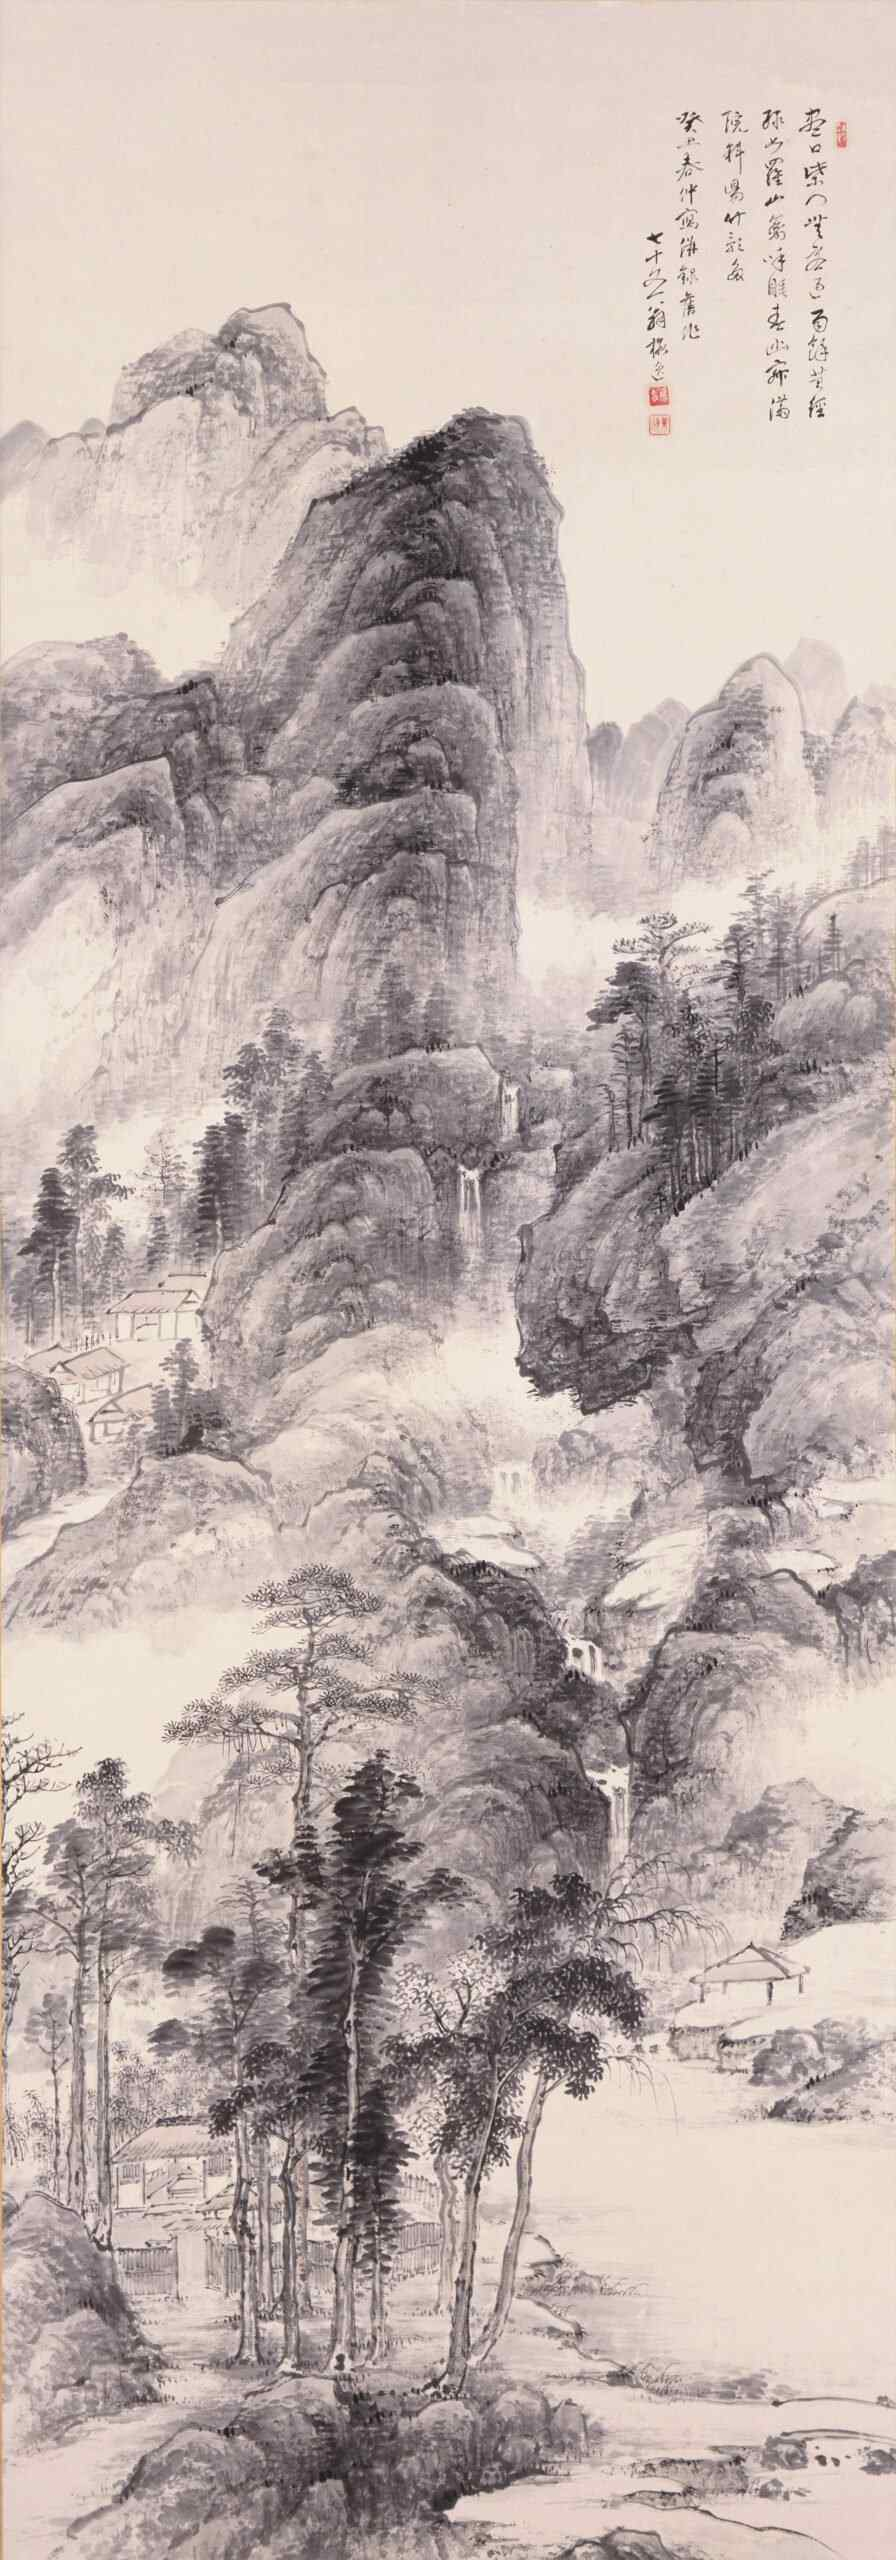
\includegraphics{../img/image04.jpg}

\begin{verseblock}

\newpage

\begin{center}\textbf{16.}\end{center}

絶 言 絶 慮 無 處 不 通

Jué yán jué lù wú chù bù tōng

Cuando cesan las palabras y el sobrepensamiento,\\
no hay lugar donde no haya claridad.

\end{verseblock}

\hfill\break

\hypertarget{comentario-15}{%
\subsection{Comentario}\label{comentario-15}}

Dejar de pensar nos parece algo difícil, casi imposible. Sin embargo,
intuimos que hay algo profundamente liberador en ello. Muchas personas,
cuando asisten por primera vez a un curso de introducción a la
meditación zen, expresan en el círculo inicial de presentación el deseo
de silenciar el ruido interno que les acompaña constantemente.

¿Cómo lograrlo? No se trata de forzar la mente al silencio ni de luchar
contra los pensamientos. El esfuerzo por acallar el pensamiento solo
genera más ruido. En lugar de eso, aprendemos a no identificarnos con el
incesante discurso mental, permitiendo que los pensamientos vengan y se
vayan sin aferrarnos a ellos. Es como sentarse a la orilla de un río y
observar el agua fluir: no intentamos detener la corriente, simplemente
la vemos pasar. De este modo, cultivamos la ecuanimidad instante tras
instante.

Nuestra tendencia natural es buscar respuestas en el conocimiento,
acumulando información con la esperanza de encontrar en ella la clave de
una vida plena y con sentido. Leemos libros, asistimos a conferencias,
buscamos maestros... Cada cual puede sustituir sabiduría por aquello que
más anhela: felicidad, éxito, amor, aceptación. Pero, ¿dónde estamos
realmente buscando?

La siguiente historia de Nasrudín ilustra con humor nuestra constante
búsqueda en el lugar equivocado:

Una noche, Nasrudín estaba dando vueltas alrededor de una farola,
mirando al suelo con atención. Un vecino que pasaba por allí le
preguntó:

---Nasrudín, ¿qué haces? ¿Has perdido algo?

---Sí, estoy buscando las llaves de mi casa.

El vecino se quedó a ayudarle. Al rato, se les unió una vecina, y luego
otro vecino más. Juntos buscaron y buscaron hasta que, cansados de no
encontrar nada, uno de ellos preguntó:

---Nasrudín, ¿estás seguro de haber perdido las llaves aquí?

---No, las perdí allí arriba.

---¡Pero entonces, ¿por qué las estamos buscando aquí?!

---Porque aquí hay más luz.

¿Cuántas veces buscamos la claridad en el lugar equivocado? Pensamos que
más conocimiento, más dinero, más fama, más... nos traerá la respuesta,
cuando en realidad la clave no está en acumular, sino en soltar.

Desde la perspectiva de la mente despierta, no hay opuestos, no hay nada
que comprender, nada que atrapar con la mente conceptual. Solo queda la
realidad tal como es.

\hfill\break

\hypertarget{02}{}
\begin{verseblock}

\newpage

\begin{center}\textbf{17.}\end{center}

歸 根 得 旨 隨 照 失 宗

Guī gēn dé zhĭ Suí zhào shī zōng

Volver al origen es alcanzar la esencia,\\
seguir las apariencias es alejarse de la realización.

\end{verseblock}

\hfill\break

\hypertarget{comentario-16}{%
\subsection{Comentario}\label{comentario-16}}

Para comprender quiénes somos realmente, debemos regresar a nuestra
raíz, en lugar de perdernos en el mundo de las apariencias y las
distracciones. La mente ordinaria se aferra a lo externo, a los nombres,
a las formas y a las identidades que construimos, olvidando que la
verdad esencial no puede atraparse con conceptos.

Nuestra percepción habitual nos extravía en la dualidad, en el vaivén
entre lo que consideramos bueno o malo, éxito o fracaso, ser o no ser.
Nos identificamos con estas distinciones y terminamos encadenados a una
visión fragmentada de la existencia. Como nos recuerda El principito:
«Lo esencial es invisible a los ojos». Lo que realmente tiene valor no
puede ser captado con la mirada superficial que aplicamos a la vida
cotidiana, sino que requiere una percepción más profunda, libre de
filtros e interpretaciones.

Este retorno a lo esencial no es un viaje hacia un lugar lejano ni el
resultado de una acumulación de conocimientos. Es, el simple acto de
estar presentes, de sentir plenamente la vida sin mediaciones. Zazen nos
ofrece este espacio de retorno, donde dejamos caer lo innecesario y nos
encontramos con la realidad tal como es. No es una abstracción ni un
ideal filosófico, sino una experiencia directa de nuestra propia
naturaleza.

Al sentarnos en quietud, sin aferrarnos a nada ni rechazar nada,
comenzamos a percibir la existencia sin adornos. Sin la necesidad de
construir una imagen de nosotros mismos ni de sostener ficciones que
refuercen nuestro ego. Es en esta desnudez, en esta autenticidad
radical, donde aflora lo que realmente somos: claridad, apertura,
presencia.

Volver al origen no significa retroceder ni perderse en el pasado.
Significa reconocer, aquí y ahora, que ya somos completos. Que no hay
nada que alcanzar, solo algo que soltar: el peso de nuestras ilusiones.
Cuando dejamos de aferrarnos a la apariencia y volvemos a la raíz,
descubrimos que lo esencial nunca ha estado perdido, simplemente estaba
oculto bajo el ruido de nuestras propias construcciones mentales.

\hfill\break

\hypertarget{03}{}
\begin{verseblock}

\newpage

\begin{center}\textbf{18.}\end{center}

須 臾 返 照 勝 卻 前 空

Xū yú făn zhào shèng què qián kōng

Cuando la luz se dirige hacia el interior,\\
en un instante, se trasciende el vacío ilusorio.

\end{verseblock}

\hfill\break

\hypertarget{comentario-17}{%
\subsection{Comentario}\label{comentario-17}}

Zazen a zazen, kinhin a kinhin, cultivamos la capacidad de dirigir la
luz de la conciencia hacia nuestro interior. Al inicio de la práctica,
la mente está envuelta en una bruma densa, un flujo incesante de
pensamientos, emociones y juicios que oscurecen la claridad natural de
nuestra consciencia. A través de la perseverancia, poco a poco la niebla
comienza a disiparse. Llega un momento en que dejamos de ser meros
observadores de la realidad y nos volvemos uno con ella. Más allá de la
forma y del vacío, más allá de la dualidad con la que solemos
interpretar la experiencia.

En el Sutra Corazón de la Gran Sabiduría recitamos que forma es vacío,
vacío es forma. Estas no son dos realidades separadas, sino expresiones
de una misma verdad. Nos perdemos cuando nos aferramos a la forma,
tomando las apariencias como si fueran entidades fijas e independientes.
Pero también nos extraviamos cuando nos apegamos a la vacuidad, creyendo
que la ausencia de sustancia es el fin último.

No se trata de rechazar la forma ni de rechazar el vacío, sino de ver
con claridad que la Realidad es una y completa en sí misma. No puede
atraparse con conceptos ni definiciones, porque en el momento en que
intentamos poseerla, desaparece, como una pompa de jabón que estalla en
el aire.

En zazen aprendemos a permanecer en la experiencia sin cristalizarla en
ideas o juicios. Cuando dirigimos la luz hacia el interior sin buscar
nada, sin intentar aferrarnos o rechazar, la dualidad se desvanece y se
revela la plenitud del instante presente. Aquí, ahora, sin necesidad de
añadir nada ni de quitar nada ni al vacío ni a la forma.

\hfill\break

\hypertarget{04}{}
\begin{verseblock}

\newpage

\begin{center}\textbf{19.}\end{center}

前 空 轉 變 皆 由 妄 見

Qián kōng zhuăn biàn jiē yóu wàng jiàn

Los cambios que parecen tener lugar en el vacío,\\
surgen de una percepción equivocada creada por la ignorancia.

\end{verseblock}

\hfill\break

\hypertarget{comentario-18}{%
\subsection{Comentario}\label{comentario-18}}

Nuestra percepción de la realidad es ilusoria, proyectamos nuestra
ignorancia en el mundo percibido. En el Budismo a este error de
percepción lo llamamos ignorancia. Esta ignorancia no está causada por
no haber estudiado, leído o reflexionado intelectualmente lo suficiente.
Es causada por un error de enfoque de la atención que crea ilusiones y
atribuye a esas ilusiones realidad absoluta. Esta manera de percibir es
el origen del sufrimiento, del
samsara\protect\hypertarget{ref1}{\protect\hyperlink{nota1}{1}}.

Desde la perspectiva de la vacuidad, el cambio es ilusión y todos
vivimos atrapados en esta ilusión colectiva, pero cuidado, rechazar la
ilusión y aferrarse a la realidad absoluta es otra forma de ilusión.
Como se dice en el Zen las cosas son lo que son, si lo comprendes son lo
que son, si no lo comprendes, siguen siendo lo que son.

Todo cambia continuamente y al mismo tiempo nada cambia, es solo una
ilusión, un sueño. No intentes entender esto, siéntate en zazen en la
actitud adecuada y la puerta de la casa del Buda se te abrirá de par en
par. El maestro Dogen en el Shôbogenzô Bendowa lo expresa así:

Si abandonamos, si olvidamos el cuerpo y el espíritu,

podremos penetrar en la casa del Buda.

\hfill\break

\hypertarget{05}{}
\begin{verseblock}

\newpage

\begin{center}\textbf{20.}\end{center}

不 用 求 眞 唯 須 息 見

Bù yòng qiú zhēn wéi xū xī jiàn

No necesitas buscar la verdad,\\
tan solo suelta las percepciones erróneas.

\end{verseblock}

\hfill\break

\hypertarget{comentario-19}{%
\subsection{Comentario}\label{comentario-19}}

Nuestro sentimiento profundo de carencia nos empuja de un lado a otro,
como un barco a la deriva, sin rumbo claro. Buscamos alcanzar un estado
de plenitud que solemos identificar con "la verdad", la perfección, la
felicidad... Cada cual se aferra a sus propias ideas ilusorias sobre
ello, verbalizándolas internamente de acuerdo con sus condicionamientos
personales. Lo normal es que este proceso suela desarrollarse de manera
completamente inconsciente.

Este sentimiento de carencia nos impulsa, con frecuencia, a perseguir
logros y gratificaciones efímeras. Que incluso cuando los alcanzamos,
lejos de llenarnos, nos dejan un vacío aún más profundo, alimentando la
frustración y la insatisfacción.

Para encontrar la "verdad", no necesitamos correr tras ella ni
fabricarla según nuestras propias representaciones. Basta con ver la
realidad tal cual es. Cuando esto sucede, la ignorancia se disuelve de
manera natural

En la tradición Soto Zen, detenemos esta carrera sin fin. Nos paramos,
nos sentamos y nos sentimos.Zazen es la actitud más adecuada para hacer
efectiva esta realización. En la quietud de la práctica, dejamos de
buscar fuera y nos abrimos a la experiencia directa de la realidad.
Recibimos y experimentamos la verdad con toda su energía y actividad. Si
dejamos ir nuestras construcciones mentales y prejuicios, podemos
fundirnos con la actividad del universo en su totalidad.

\hfill\break

\begin{center}\rule{0.5\linewidth}{0.5pt}\end{center}

\leavevmode\vadjust pre{\hypertarget{notas}{}}%
\textsuperscript{1} En el budismo se corresponde con el sufrimiento,
propio del mundo material, del que los seres humanos son los únicos
seres renacidos dentro de los Seis reinos del samsara, que son capaces
de distanciarse, mediante la liberación, y, posteriormente, de
separarse, mediante el nirvana. El tiempo necesario para liberarse del
samsara depende de las prácticas espirituales y del karma acumulado en
vidas anteriores \protect\hyperlink{ref1}{Volver}

\hfill\break

\hypertarget{01}{}
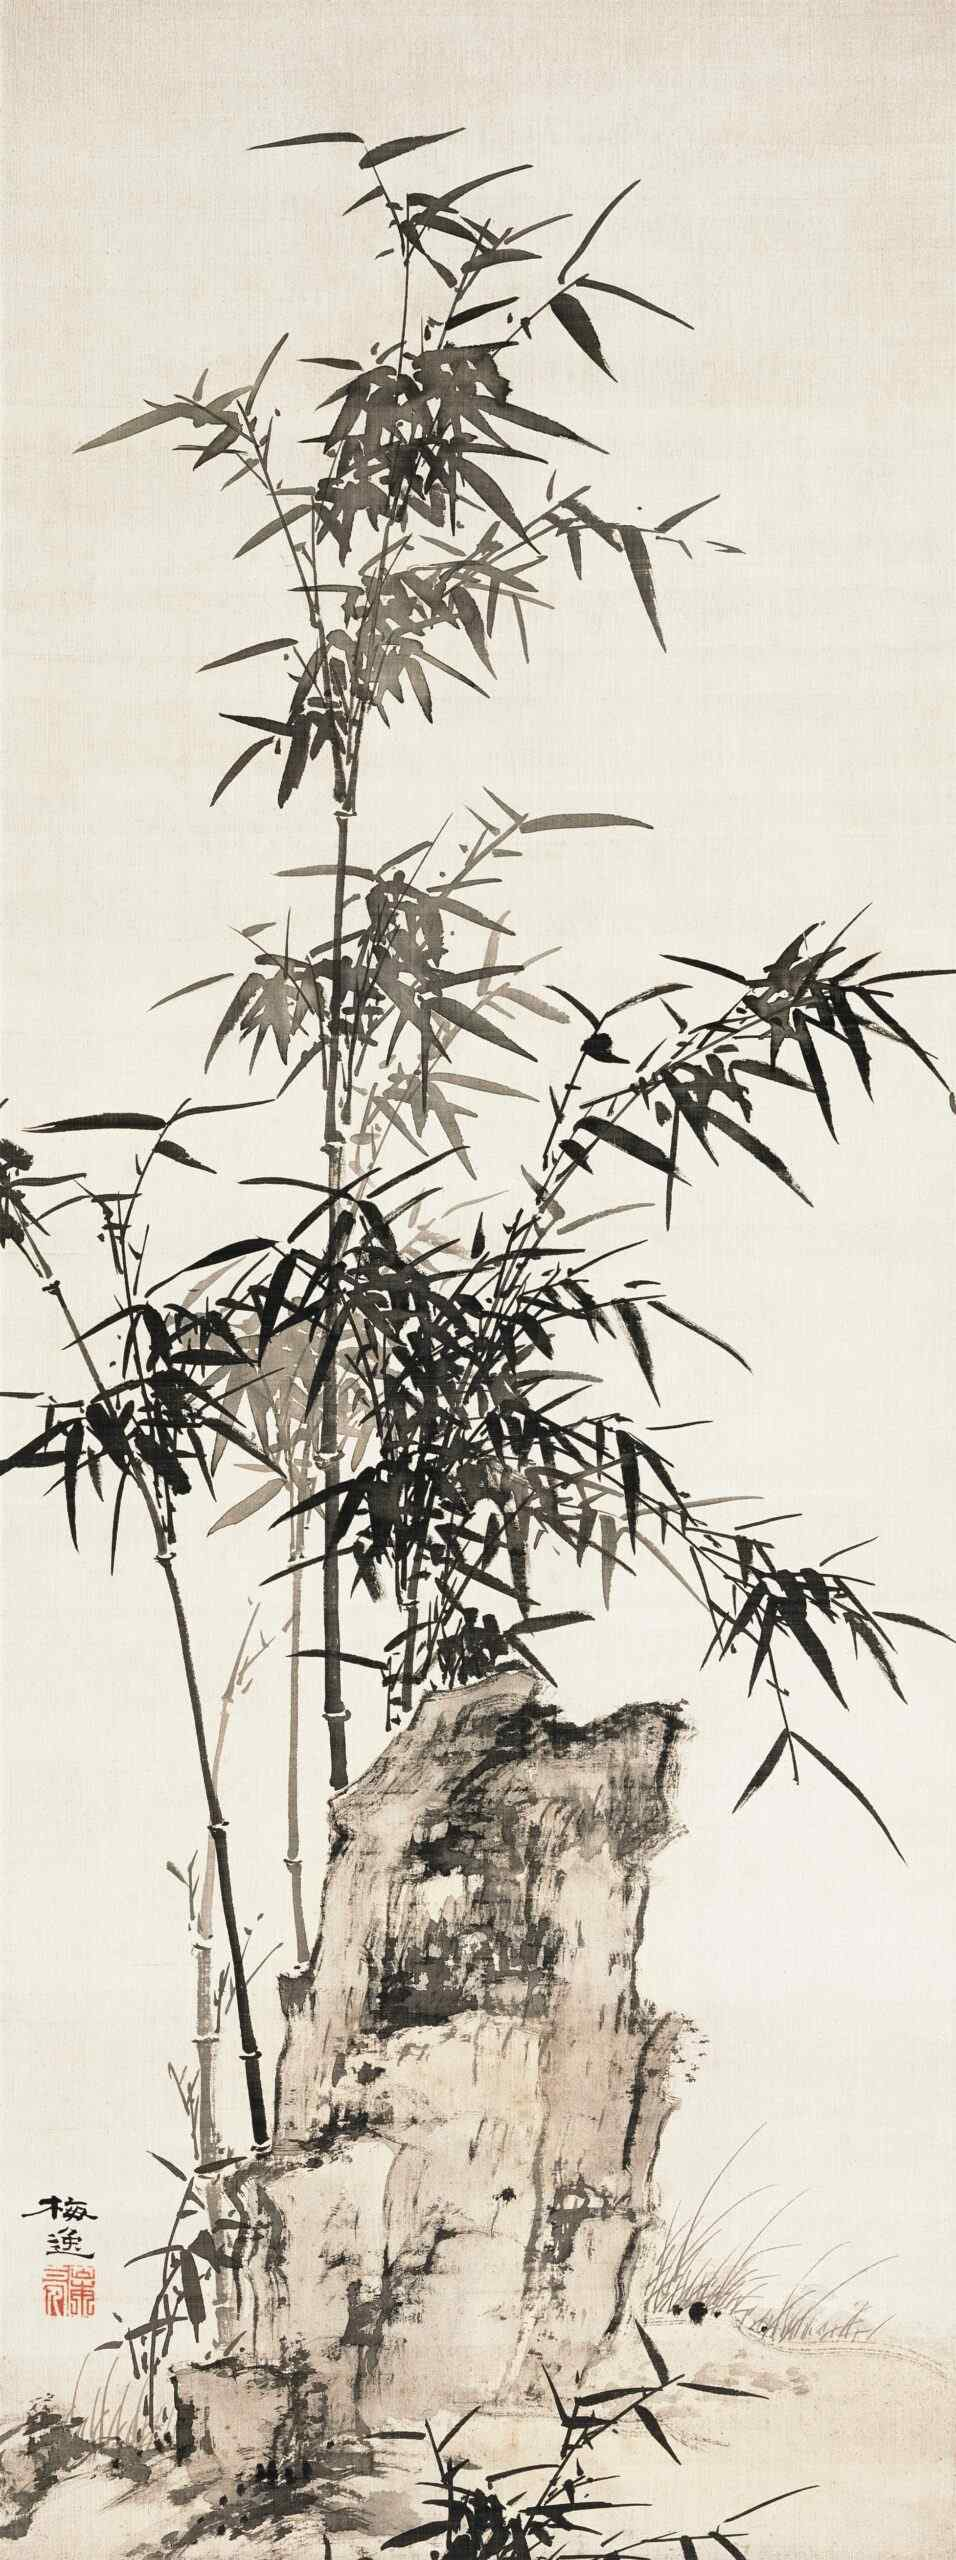
\includegraphics{../img/image05.jpg}

\begin{verseblock}

\newpage

\begin{center}\textbf{21.}\end{center}

二 見 不 住 慎 莫 追 尋

Èr jiàn bù zhù shèn mò zhuī xún

No te aferres a puntos de vista dualistas,\\
actúa con cuidado y no los persigas.

\end{verseblock}

\hfill\break

\hypertarget{comentario-20}{%
\subsection{Comentario}\label{comentario-20}}

Las
dicotomías\textsuperscript{\protect\hypertarget{ref1}{\protect\hyperlink{nota1}{1}}}
son la base de nuestra percepción automática de la realidad.
Inconscientemente, necesitamos identificarnos con uno de los extremos
para autoconvencernos de que el constructo que llamamos ``Yo'' es real.
La tradición budista nos enseña que el ego es un constructo mental
imaginario. El ``Yo y lo mío'' son necesarios para desenvolvernos en
nuestra vida cotidiana, pero al fin y al cabo son una construcción
carente de realidad intrínseca. Ello provoca un sentimiento de carencia,
de sed de existencia, que nos acompaña continuamente, seamos conscientes
de ello o no.

Una de las estrategias inconscientes que utilizamos para evitar el
sentimiento de vacío provocado por este falso ``Yo'' es apegarnos a uno
de los extremos en los que escindimos la realidad. Este apego nos da una
falsa sensación de Ser, la cual nos provoca una gran cantidad de
problemas asociados a esta identificación. Ya que se convierte en algo
tan fundamental para nosotros que mantenernos aferrados a ello lo
llegamos a considerar una cuestión de vida o muerte. Efectivamente, es
la vida o la muerte de un ente imaginario que hemos creado, mantenemos
vivo en nuestra imaginación y que creemos ser.

El despertar es el fin de las imaginaciones que nos hacemos sobre la
realidad, el fin de lo que creemos ser para ser lo que realmente somos.
Nuestra verdadera naturaleza está aquí y ahora en cada instante,
esperando a ser actualizado a través de la toma de conciencia de este
proceso para aprender a liberarnos de estos apegos inútiles,
insatisfactorios y dañinos.

Por tanto, ``actúa con cuidado y no los persigas''. Es decir, tomar
conciencia de a qué te estás aferrando y deja caer todos los apegos a
los que te identificas irracionalmente, ser honesto y soltar todo
aquello que no te aporte paz y felicidad a ti mismo y a todos los seres
que te rodean.

\hfill\break

\hypertarget{02}{}
\begin{verseblock}

\newpage

\begin{center}\textbf{22.}\end{center}

纔 有 是 非 紛 然 失 心

Cái yŏu shì fēi fēn rán shī xīn

Apenas surge el juicio de correcto e incorrecto,\\
mente y corazón se pierden en la confusión.

\end{verseblock}

\hfill\break

\hypertarget{comentario-21}{%
\subsection{Comentario}\label{comentario-21}}

¿Correcto, incorrecto? ¿Quién sabe las vueltas que da la vida? En vez de
aferrarnos al juicio, es más apropiado desarrollar una actitud de
aceptación. Si te gusta, las cosas son como son; si no te gusta, las
cosas son como son. Nos pasamos la vida enjuiciando, atrapados en una
corriente incesante de opiniones y evaluaciones, lo que nos desconecta
de nuestro corazón, de nuestra verdadera mente, de lo que realmente
somos. Así nos sumimos en la confusión.

Sin embargo, en la vida cotidiana es inevitable elegir. En cada momento
tomamos decisiones, grandes o pequeñas, que dan forma a nuestro camino.
Lo que la práctica nos proporciona no es una evasión de la
responsabilidad, sino la claridad y la sabiduría necesarias para elegir
con mayor lucidez, sin quedar atrapados en el miedo, el apego o la
confusión.

¿Cómo salir de este callejón sin salida? A través de la visión despierta
que surge con la práctica de zazen. Al cultivar la bondad, la compasión,
la alegría y la ecuanimidad, aprendemos a relacionarnos con la realidad
de manera más natural y sabia, en armonía con cada momento. De este
modo, la niebla de la ofuscación se disipa, y con ello ganamos
estabilidad emocional y mental, algo esencial para conectar con nuestra
bondad innata y vivir el día a día con un corazón tranquilo, en paz y
libre.

Se trata de soltar la compulsión, de clasificar cada experiencia como
buena o mala y, en su lugar, habitar la realidad con una apertura total.
¿Cómo se experimenta esto en la vida cotidiana? En la capacidad de
recibir cada instante sin etiquetarlo, de sostener el mundo sin el
filtro del «yo y lo mío», sin imponer una narrativa sobre lo que debería
ser. Y cuando llegue el momento de decidir, hacerlo desde la sabiduría,
con la mente despejada y el corazón en paz.

\hfill\break

\hypertarget{03}{}
\begin{verseblock}

\newpage

\begin{center}\textbf{23.}\end{center}

二 由 一 有 一 亦 莫 守

Èr yóu yī yŏu yī yì mò shŏu

Aunque la dualidad surge de la unidad,\\
tampoco te aferres a la unidad.

\end{verseblock}

\hfill\break

\hypertarget{comentario-22}{%
\subsection{Comentario}\label{comentario-22}}

La Realidad no puede ser capturada por el lenguaje, al utilizar el
lenguaje para representar la realidad nos obliga a expresarnos en
términos de unidad y dualidad. Sin una, la otra no puede existir, la
verdadera unidad no se limita a negar la dualidad: la abarca y la
trasciende. Si nos aferramos a la idea de unidad como opuesta a la
dualidad, seguimos atrapados en una forma de pensamiento fragmentado. La
verdadera comprensión no consiste en elegir entre una y otra, sino en
ver que ambas son expresiones de una misma realidad.

¿Cómo podemos aplicar esto a nuestra práctica? El maestro Dogen Zenji
nos ofrece una clave fundamental en el
Fukanzazengi\textsuperscript{\protect\hypertarget{ref2}{\protect\hyperlink{nota2}{2}}}:

«Para hacer zazen conviene un espacio silencioso. Come y bebe
sobriamente. Despréndete de cualquier compromiso y abandona toda
preocupación. No pienses: `Esto está bien, esto está mal'. No tomes
partido ni por ni contra. Detén todo movimiento de tu mente consciente.
No juzgues los pensamientos que aparecen. No cultives expectativas. No
tengas ningún deseo de llegar a ser Buda.»

Estas palabras nos muestran que la práctica no consiste en elegir un
lado, sino en dejar que la realidad se revele sin filtros ni juicios.
Soltando nuestras fijaciones y no dividiendo la experiencia en bueno o
malo, correcto o incorrecto, etc. Solo así podemos asentarnos en una
presencia que no se aferra ni rechaza, sino que simplemente es.

Al no tomar partido «ni por ni contra», con una mente abierta y
flexible, podemos experimentar la unidad dentro de la diversidad y
reconocer en la diversidad la unidad esencial de todas las cosas. Lo que
a simple vista parecen opuestos ---bien y mal, luz y sombra, vacío y
forma--- no son más que diferentes manifestaciones de la misma realidad
interdependiente.

1 0-+

El propio Dogen, al regresar de China tras recibir la transmisión del
Dharma, fue preguntado sobre qué traa consigo. En lugar de volver
cargado de sutras, como era costumbre entre los monjes de su tiempo,/
respondió:

«He vuelto con las manos vacías, pero con una mente abierta y flexible.»

Esta es la esencia de la práctica: soltar toda fijación y permitir que
la realidad se manifieste tal como es. No se trata de acumular
conocimientos o aferrarse a conceptos elevados, sino de dejar ir toda
preconcepción y estar presentes en lo que surge momento a momento.

Cuando comprendemos esto en nuestra práctica diaria, podemos ver que la
verdadera unidad no es una idea abstracta ni un estado que deba
alcanzarse. Es la vida misma tal como es, aquí y ahora. En cada
respiración, en cada paso, en cada interacción con otras personas y con
el mundo, la unidad se expresa en la infinita diversidad de formas.

Así, sin rechazar la dualidad ni aferrarnos a la unidad, caminamos por
la vía del despertar con una actitud de apertura, humildad y confianza
en la naturaleza de todas las cosas.

\hfill\break

\hypertarget{04}{}
\begin{verseblock}

\newpage

\begin{center}\textbf{24.}\end{center}

一 心 不 生 萬 法 無 咎

Yī xīn bù shēng wàn fă wú jiù

Cuando la mente no construye,\\
los diez mil fenómenos están libres de error.

\end{verseblock}

\hfill\break

\hypertarget{comentario-23}{%
\subsection{Comentario}\label{comentario-23}}

En el budismo Mahayana, y en particular en el Sutra del Diamante, se
habla de la mente unificada como un estado de conciencia en el que se
alcanza la comprensión profunda de la verdadera naturaleza de la
realidad. Este estado no es una abstracción filosófica, sino una
experiencia directa en la que se disuelven las construcciones
conceptuales y se perciben los fenómenos tal como son:
interdependientes, vacíos de existencia inherente y en constante cambio.
La mente unificada no es una idea que pueda captarse intelectualmente,
sino una vivencia que surge cuando se trasciende la dualidad entre
sujeto y objeto.

En la mente unificada, no hay una búsqueda de lo placentero ni un
rechazo de lo desagradable, porque ambas tendencias surgen del apego a
una idea del «yo» que se enfrenta a la realidad como si fuera algo
separado de ella. En la vida cotidiana, esta ilusión de separación nos
lleva al sufrimiento al crear expectativas y resistencias innecesarias.
Observar cómo estas tendencias emergen y se disuelven en la práctica es
parte esencial del camino.

La mente unificada es la actualización viviente de la vacuidad, tal como
la enseña el Sutra del Corazón: «La forma es vacío y el vacío es forma».
No significa una mente en blanco o una pasividad sin dirección, sino una
claridad sin obstrucciones, como un espejo que refleja sin distorsionar.
En el Shôbôgenzô Ikka Myoju, Dōgen afirma:

«El universo entero es una perla brillante.»

Esta metáfora expresa la perfección inherente de la realidad tal como
es. Nada sobra, nada falta. Así como la perla refleja todo sin
distorsión, la mente unificada no altera la realidad con juicios o
preferencias, sino que todo lo refleja tal como es. Sentarse en la paz
de zazen, dejarse caer hasta el fondo de uno mismo, es la actualización
de esta enseñanza. No es un concepto, sino una vivencia que solo puede
realizarse a través de la práctica continuada.

Cuando la mente está unificada, los «diez mil fenómenos» ---todo lo que
existe--- aparecen tal como son, sin distorsiones ni errores de
interpretación. No hay juicio ni separación, solo la íntima comprensión
de que la mente y los fenómenos no son dos. Este es el estado en el que
el Dharma se revela en cada instante, en cada respiración, en cada
sonido del viento entre los árboles.

Así, la mente unificada no es un objetivo que alcanzar en el futuro,
sino la condición natural que se manifiesta cuando dejamos de
resistirnos a lo que es. La práctica del budismo Soto Zen no busca
fabricar un estado especial, sino disolver las obstrucciones que nos
impiden ver que la Vía ya está presente en cada momento, el aquí y
ahora, el eterno presente. Cada vez que nos sentamos en zazen, dejamos
de resistirnos y permitimos que la mente unificada se manifieste,
recordándonos que el aquí y ahora es el único momento en el que la Vía
puede vivirse plenamente.

\hfill\break

\hypertarget{05}{}
\begin{verseblock}

\newpage

\begin{center}\textbf{25.}\end{center}

無 咎 無 法 不 生 不 心

Wú jiu wú fă Bù shēng bù xīn

Sin error, no hay fenómenos.\\
Sin construcciones mentales, no hay apego ni rechazo.

\end{verseblock}

\hfill\break

\hypertarget{comentario-24}{%
\subsection{Comentario}\label{comentario-24}}

Los errores y las construcciones mentales no son ajenos a la existencia;
más bien, la hacen posible. Son como el anverso y el reverso de una
misma moneda: sin ellos, no habría fenómenos ni mente que los perciba.
Sin embargo, estas construcciones surgen de la ignorancia y la ilusión,
generando divisiones donde no las hay, atrapándonos en la dualidad y el
conflicto.

El sufrimiento surge cuando confundimos nuestras interpretaciones con la
realidad misma. Al aferrarnos a nuestras proyecciones mentales, nos
perdemos en el juego de las oposiciones: correcto e incorrecto, bueno y
malo, apego y rechazo. Pero si dejamos de alimentar esas construcciones
erróneas, la realidad se muestra sin fisuras, sin necesidad de ser
dividida en opuestos.

La práctica de zazen nos permite experimentar esta claridad
directamente. No se trata de erradicar la percepción o el pensamiento,
sino de reconocer su naturaleza y no quedar atrapados en ellos. En lugar
de eliminar todas las construcciones mentales, aprendemos a verlas por
lo que son, liberándonos de aquellas que nos ciegan y cultivando una
mente abierta, serena y compasiva.

Cuando la mente deja de proyectar sus distorsiones, los fenómenos no se
presentan como separados ni en conflicto. La realidad es una,
indivisible, pero es nuestra percepción errónea la que genera la ilusión
de lo múltiple y fragmentado. Ver con claridad es liberarnos de esa
distorsión y, en esa liberación, ser uno con nuestra naturaleza
original.

\hfill\break

\begin{center}\rule{0.5\linewidth}{0.5pt}\end{center}

\leavevmode\vadjust pre{\hypertarget{notas}{}}%
\textsuperscript{1} División de un concepto o una materia teórica en dos
aspectos, especialmente cuando son opuestos o están muy diferenciados
entre sí. \protect\hyperlink{ref1}{Volver}

\textsuperscript{2} Fukanzazengi, ``Para la difusión universal de los
principios de zazen'', del maestro zen Eihei Dôgen (1200-1254).
\protect\hyperlink{ref2}{Volver}

\hfill\break

\hypertarget{01}{}
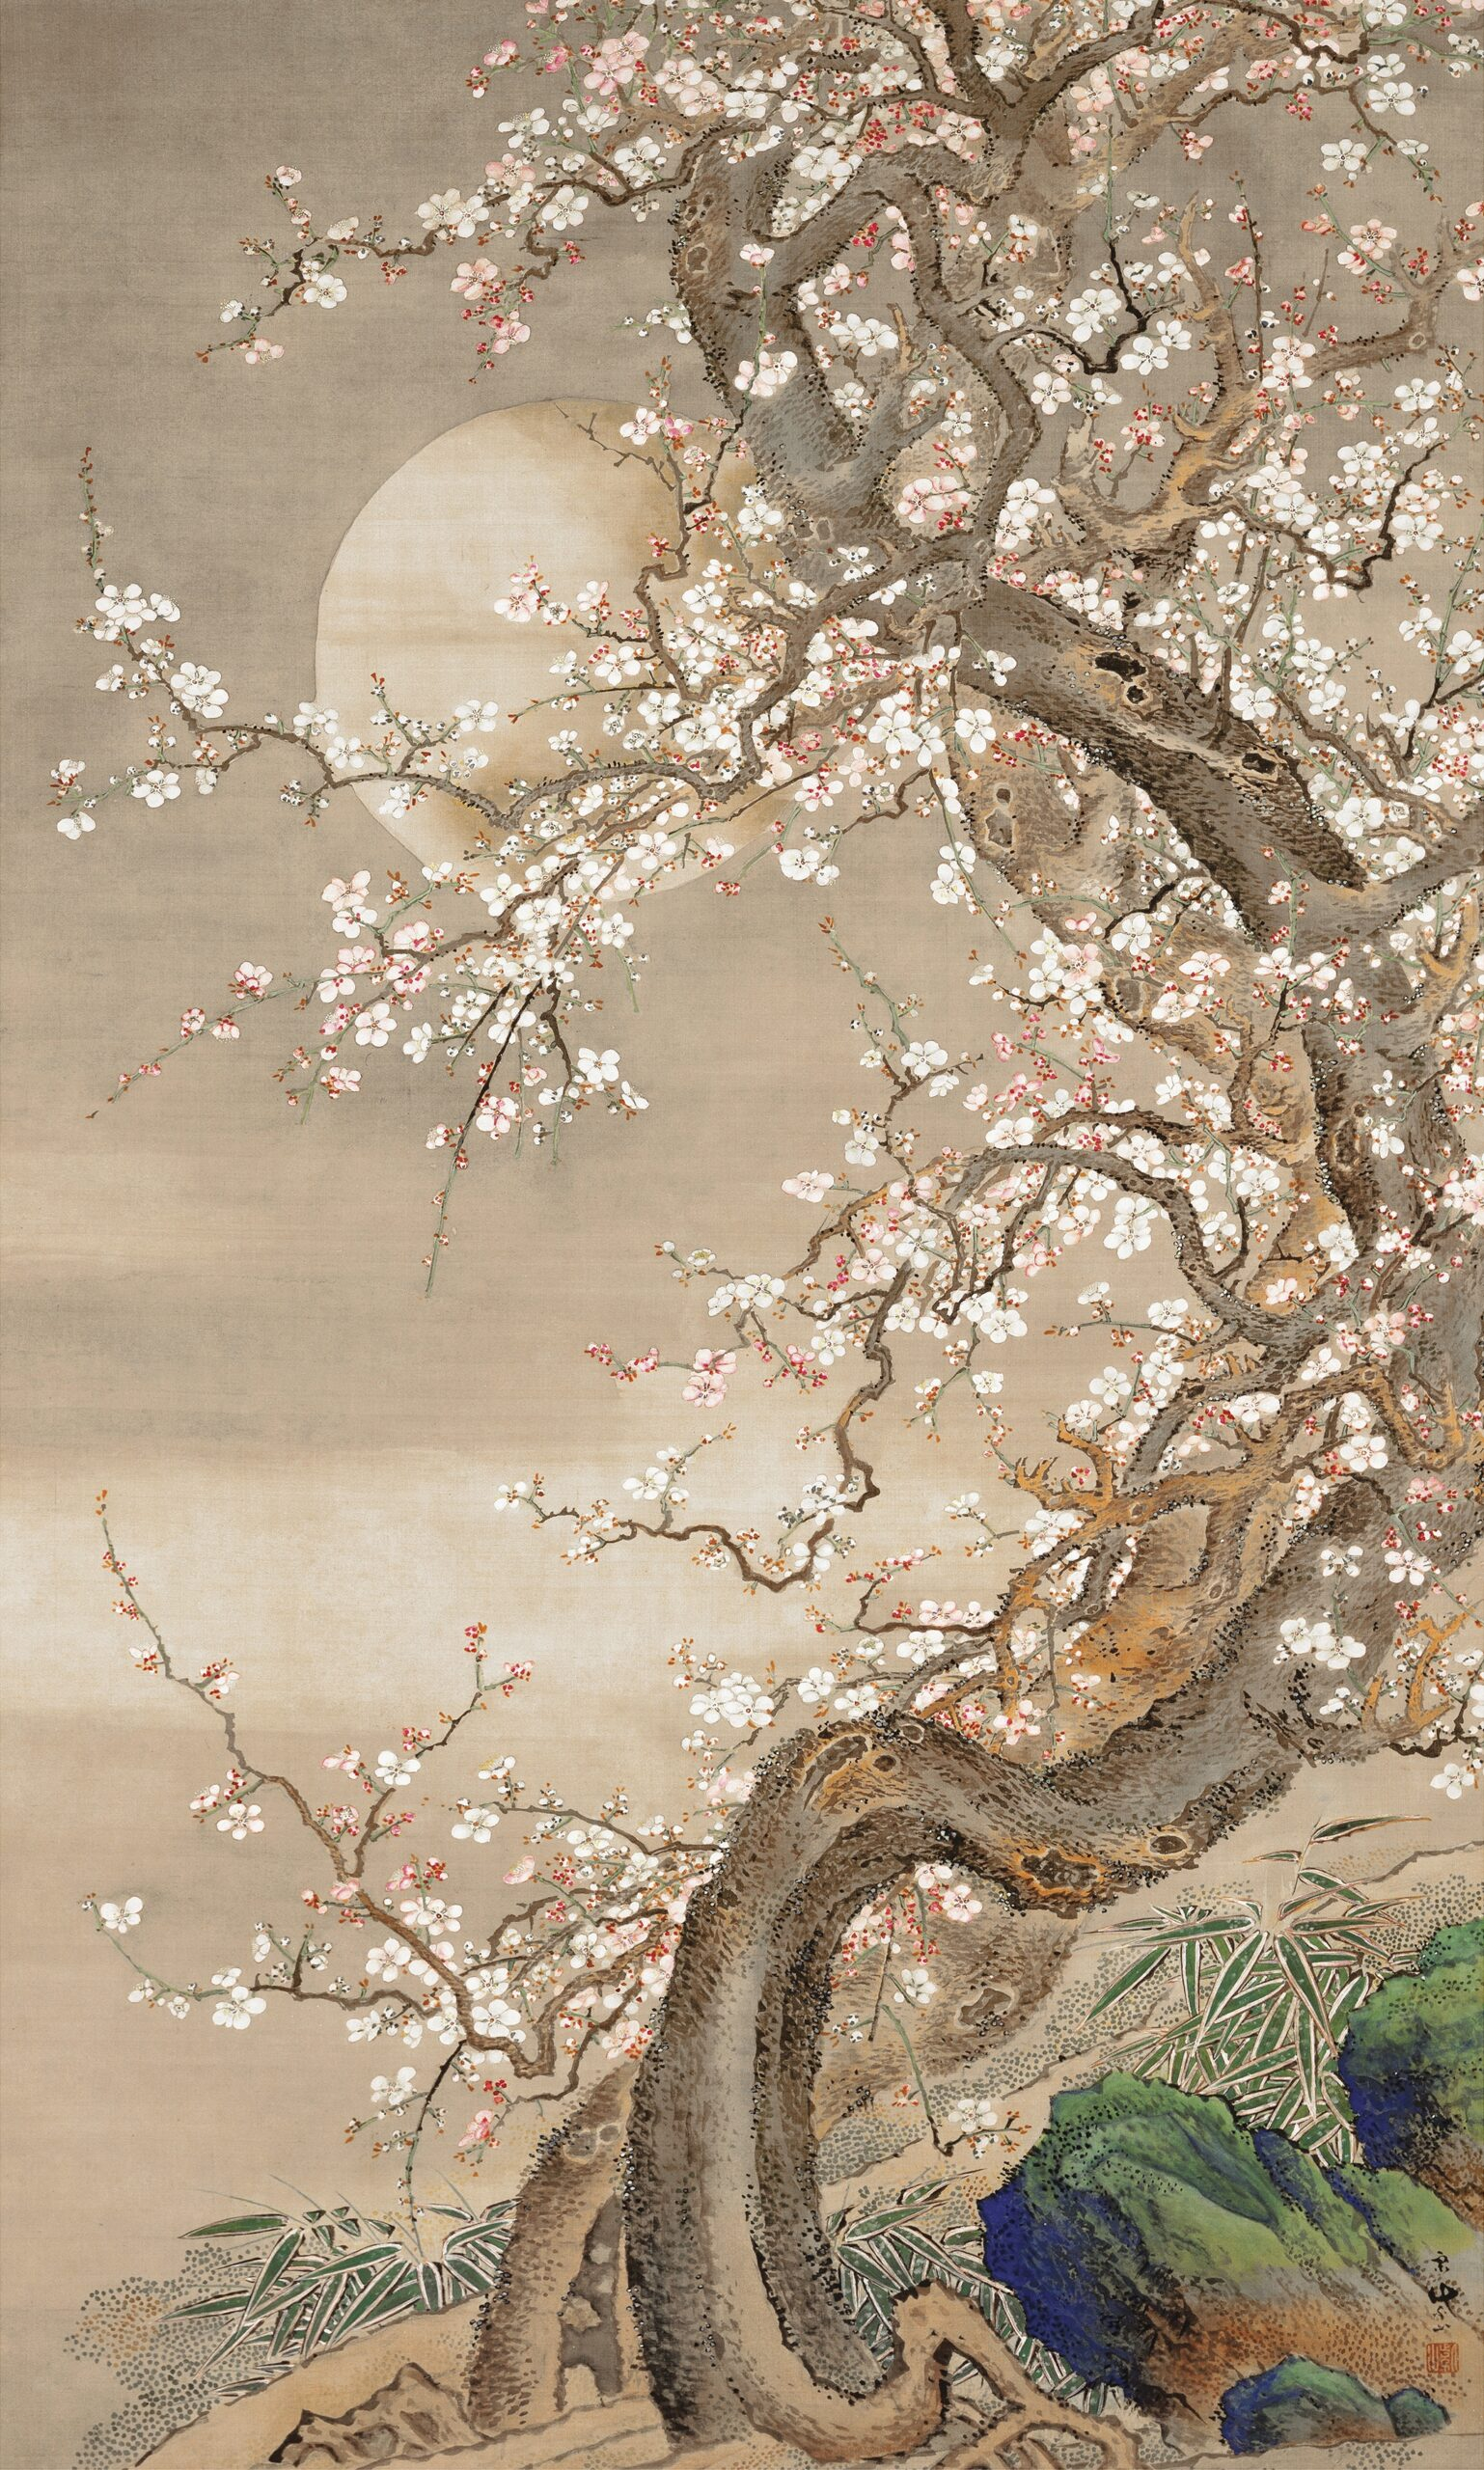
\includegraphics{../img/image06.jpg}

\begin{verseblock}

\newpage

\begin{center}\textbf{26.}\end{center}

能 隨 境 滅 境 逐 能 沈

Néng suí jìng miè Jìng zhú néng chén

La ecuanimidad se puede desvanecer con las circunstancias.\\
Persiguiendo las circunstancias nos perdemos en la confusión.

\end{verseblock}

\hfill\break

\hypertarget{comentario-25}{%
\subsection{Comentario}\label{comentario-25}}

La ecuanimidad es un estado de calma profunda que surge naturalmente con
la práctica correcta de zazen, pero que puede desvanecerse cuando las
circunstancias cambian. Cuando estamos bien, creemos que podemos
mantenernos serenos en cualquier momento, pero cuando las condiciones
dejan de ser favorables, cuando algo nos inquieta, cuando nos
identificamos con ello y nos arrastra, entonces es fácil ver cómo esa
estabilidad se disuelve. Si la ecuanimidad depende de lo que ocurre
fuera de nosotros, en realidad no es ecuanimidad, sino un espejismo
frágil que se quiebra con el más mínimo viento.

Cuanto más nos aferramos a las condiciones externas, cuanto más
intentamos ajustar la realidad a nuestros deseos, más nos alejamos de la
claridad. La mente atrapada en el ir y venir de los acontecimientos se
vuelve como una marioneta que salta al ritmo de lo que ocurre fuera,
incapaz de sostenerse por sí misma. En la práctica del budismo Soto Zen,
la estabilidad no surge de encontrar el entorno perfecto o de evitar lo
que nos incomoda, sino de cultivar una presencia atenta y una aceptación
profunda de lo que es.

Cuando nos dejamos llevar por el flujo interminable de las
circunstancias, la mente se agita, la confusión se intensifica y la
serenidad se vuelve un recuerdo distante. Pero hay otra manera de ser y
estar en el mundo: habitar el cambio sin ser arrastrados por él. No se
trata de insensibilidad ni de indiferencia, sino de aprender a habitar
el presente sin depender de que las cosas sean de una manera u otra.
Solo entonces, la ecuanimidad deja de ser un concepto y se convierte en
una forma de estar en el mundo.

\hfill\break

\hypertarget{02}{}
\begin{verseblock}

\newpage

\begin{center}\textbf{27.}\end{center}

境 由 能 境 能 由 境 能

Jìng yóu néng jìng Néng yóu jìng néng

El objeto depende del sujeto, el sujeto depende del objeto.\\
Sujeto y objeto se originan mutuamente.

\end{verseblock}

\hfill\break

\hypertarget{comentario-26}{%
\subsection{Comentario}\label{comentario-26}}

El objeto depende del sujeto, es decir, la realidad no es algo fijo e
independiente de nuestra percepción. Todo lo que experimentamos está
condicionado por nuestra mente, nuestra historia personal y nuestra
manera de interpretar el mundo. No hay un mundo externo objetivo que
simplemente esté ahí, esperando ser visto de una única manera; lo que
llamamos ``objeto'' surge en relación con el sujeto que lo experimenta.

A su vez, el sujeto depende del objeto. No existe un "yo" separado de lo
que percibe. Somos, en gran medida, las experiencias que tenemos, la
relación que establecemos con lo que nos rodea. Nuestra identidad se
define en el encuentro con el mundo, en la interacción con cada cosa que
surge en nuestra conciencia. Si no hubiera objetos de percepción, ¿qué
sentido tendría hablar de un sujeto?

Sujeto y objeto se originan mutuamente, no es solo que uno dependa del
otro, sino que emergen juntos, inseparables. No hay un antes ni un
después, no hay un sujeto puro que primero existe y luego encuentra un
mundo externo, ni un mundo independiente que precede a la conciencia.
Todo aparece en relación. En la práctica de zazen, cuando la
concentración se estabiliza en el objeto primario de atención, ya no hay
un observador separado de la respiración, del sonido del viento, de la
sensación del cuerpo sobre el suelo.

Si realizamos profundamente esta enseñanza, la rigidez con la que nos
aferramos a nuestra identidad y a la realidad que creemos inmutable
comienza a disolverse. No somos entes aislados mirando un mundo desde
fuera, ni tampoco somos meras reacciones a lo que ocurre. Somos
relación, somos interdependencia, somos la actividad misma de surgir
junto con todo lo que es.

La realidad es una red interconectada de fenómenos y nuestra percepción
está intrincadamente entrelazada con la realidad misma. La práctica del
budadharma nos lleva a contemplar esta interdependencia y a desarrollar
una comprensión más profunda de la naturaleza relativa de las cosas,
trascendiendo así la ilusión de una existencia separada y alcanzando una
visión más clara de la verdadera naturaleza de la realidad y de nosotros
mismos.

\hfill\break

\hypertarget{03}{}
\begin{verseblock}

\newpage

\begin{center}\textbf{28.}\end{center}

欲 知 兩 段 元 是 一 空

Yù zhī liăng duàn yuán shì yī kōng

Si se quiere comprender las dos partes,\\
su origen es el mismo: vacío.

\end{verseblock}

\hfill\break

\hypertarget{comentario-27}{%
\subsection{Comentario}\label{comentario-27}}

Para comprender las partes de los opuestos, debemos indagar en su origen
común: la vacuidad. En la tradición budista, la vacuidad no se refiere a
un vacío frío e inhóspito, sino a la ausencia de una existencia
inherente y autónoma en cada uno de los fenómenos. Todo lo que surge lo
hace en dependencia de causas y condiciones, sin una esencia propia que
lo haga fijo o permanente. No hay una identidad separada que sustente
los opuestos de manera absoluta; su existencia es relacional,
interdependiente.

Las dualidades que solemos percibir ---luz y oscuridad, bien y mal, yo y
el otro--- no son entidades fijas, sino expresiones de una misma
realidad interconectada. Surgen de la mente que discrimina y
conceptualiza, pero en sí mismas carecen de una existencia propia. Al
examinarlas con profundidad, descubrimos que no pueden sostenerse sin su
contrario: la luz no tiene significado sin la oscuridad, el sonido sin
el silencio, la forma sin el vacío. Cada fenómeno es lo que es solo en
relación con lo que no es.

Al reconocer la vacuidad de los fenómenos, nuestra percepción de la
realidad se vuelve más amplia y flexible. La vacuidad nos ayuda a
comprender que nada es sólido, separado o definitivo. Cuando nos
aferramos a las cosas como si tuvieran una identidad fija, creamos
sufrimiento, porque la realidad fluye constantemente, sin detenerse en
ninguna estructura permanente.

En la práctica budista, el reconocimiento de la vacuidad nos libera de
la rigidez de las categorías mentales y nos abre a una comprensión más
profunda de la interconexión de todos los fenómenos. Cuando comprendemos
que sujeto y objeto surgen de la misma vacuidad, desaparece la frontera
ilusoria entre el yo y los demás, entre lo interno y lo externo. De esta
comprensión surge una visión más compasiva, porque dejamos de vernos a
nosotros mismos como entidades aisladas y reconocemos nuestra
participación en un entramado infinito de interdependencia.

Trascender la dualidad no significa negar la diversidad de la
experiencia, sino integrarla con plena conciencia de su naturaleza
vacía. En la vacuidad, cada fenómeno es libre de manifestarse sin la
carga de una identidad fija, sin la prisión de un yo separado. Ver esto
con claridad nos permite habitar el mundo sin apego ni rechazo,
cultivando una sabiduría que fluye con la vida en su totalidad.

\hfill\break

\hypertarget{04}{}
\begin{verseblock}

\newpage

\begin{center}\textbf{29.}\end{center}

一 空 同 兩 齊 含 萬 象

Yī kōng tóng liăng qí hán wàn xiàng

Lo uno y el vacío son lo mismo,\\
y ambos incluyen los diez mil fenómenos.

\end{verseblock}

\hfill\break

\hypertarget{comentario-28}{%
\subsection{Comentario}\label{comentario-28}}

En la vacuidad, la aparente separación entre sujeto y objeto se
disuelve, revelando la interconexión de todos los fenómenos. La vacuidad
no significa que los fenómenos no existan, sino que carecen de una
existencia inherente y autónoma. Todo surge en dependencia de
condiciones y relaciones. Así, cuando se reconoce la verdadera
naturaleza vacía de los fenómenos, se comprende que el sujeto que
percibe y el objeto percibido no son entidades separadas, sino
manifestaciones interdependientes de una misma realidad.

Desde la perspectiva de la verdad absoluta
\textsuperscript{\protect\hypertarget{ref1}{\protect\hyperlink{nota1}{1}}},
no hay una esencia fija que sostenga la distinción entre sujeto y
objeto. Estos no son realidades separadas, sino que emergen y se
sostienen mutuamente dentro de la red infinita de interdependencia. En
este nivel de comprensión, cualquier distinción entre ambos es meramente
conceptual y carece de una base sólida. Al reconocer esto, la ilusión de
la dualidad se desvanece y nos abrimos a una experiencia directa de
unidad, donde la realidad se manifiesta libre de etiquetas y
separaciones.

Pero esta comprensión no niega la verdad relativa, el nivel en el que
operamos en nuestra vida cotidiana. En este ámbito, seguimos
interactuando con el mundo a través de distinciones funcionales:
diferenciamos entre personas, objetos, acciones y consecuencias. Aquí,
sujeto y objeto siguen existiendo convencionalmente, y el lenguaje nos
permite comunicarnos y actuar en el mundo. La verdad relativa no es un
error ni una ilusión en el sentido de algo falso, sino la forma en que
la realidad se nos presenta de manera práctica y operativa.

La verdad relativa y la verdad absoluta no son realidades separadas ni
opuestas. No es que la verdad absoluta revele una dimensión superior,
mientras que la verdad relativa sea meramente ilusoria. La verdad
relativa es la expresión misma de la verdad absoluta. Como señala
Nagarjuna: «La enseñanza de la vacuidad está basada en el camino medio;
aquellos que la malinterpretan como nihilismo son irremediablemente
incurables.''

Es precisamente debido a la vacuidad que los fenómenos pueden surgir y
relacionarse sin estar atados a una esencia fija. Los diez mil
fenómenos, en su multiplicidad y diversidad, no están separados del
vacío; son su manifestación concreta. Lo uno y lo múltiple no se
excluyen: el vacío no es una negación de la existencia, sino la ausencia
de una existencia independiente y autosustentada. Por ello, al ver la
vacuidad de todos los fenómenos, no caemos en el extremo del nihilismo,
sino que comprendemos que cada instante de nuestra experiencia es la
totalidad manifestándose plenamente.

Comprender esto nos permite vivir sin aferrarnos a una visión rígida de
la realidad. No es necesario negar la existencia convencional de los
fenómenos, pero tampoco debemos tomarlos como absolutos. Los diez mil
fenómenos y la vacuidad son lo mismo: cada ola en el océano es agua, y
sin embargo, cada ola es única en su forma y movimiento.

Este equilibrio nos permite movernos por el mundo con claridad, sin
quedarnos atrapados en la dualidad ni en la fijación de un yo separado.
Al integrar ambas perspectivas, podemos actuar con mayor sabiduría y
compasión, sabiendo que todo está interconectado y que la realidad es
libre y fluida.

\hfill\break

\hypertarget{05}{}
\begin{verseblock}

\newpage

\begin{center}\textbf{30.}\end{center}

不 見 精 麁 寧 有 偏 黨

Bù jiàn jīng cū níng yŏu piān dăng

Si no diferencias lo sutil de lo burdo,\\
¿Cómo podrías tomar partido hacia uno de los lados?

\end{verseblock}

\hfill\break

\hypertarget{comentario-29}{%
\subsection{Comentario}\label{comentario-29}}

Cuando no hacemos distinciones rígidas entre lo sutil y lo grosero, es
decir, cuando no clasificamos las experiencias o situaciones en
categorías de «bueno» o «malo», «correcto» o «incorrecto», se vuelve
innecesario tomar partido o tomar una postura rígida, inamovible.

Al no tener una visión dualista y juzgar las cosas en términos opuestos
entre sí, podemos cultivar una actitud más equilibrada y comprensiva.
Reconocemos que la vida y las situaciones son complejas y están
compuestas por múltiples matices. En lugar de aferrarnos a una
perspectiva fija, podemos abrazar la fluidez y la ambigüedad de las
circunstancias.

No tomando partido, evitamos la tendencia a generar conflictos, juicios
o divisiones. Nos abrimos a una mayor comprensión, empatía y aceptación
de la diversidad de perspectivas y experiencias. Esto nos permite
encontrar un espacio de armonía y calma al reconocer que la realidad es
mucho más amplia y compleja de lo que nuestras categorías limitadas
pueden captar.

De nuevo nos estamos refiriendo a ello desde la verdad absoluta. Pero,
incluso en la verdad relativa, donde la toma de partido es obligada,
podemos adoptar una postura más flexible y abierta, evitando la
polarización y el extremismo. Podemos buscar un enfoque más comprensivo,
escuchando y considerando diferentes puntos de vista, y reconociendo la
complejidad inherente de muchas situaciones. No aferrándonos rígidamente
a la visión dicotómica de la realidad y no cayendo en juicios
simplistas. Reconociendo que hay múltiples perspectivas, matices y
factores a considerar en cualquier situación.

Al generar una actitud comprensiva y abierta, cultivamos un estado
interno pacífico que se irradia hacia nuestras interacciones y
relaciones con los demás, creando un entorno de armonía y compasión para
el bien de todos los seres, incluidos nosotros mismos.

\hfill\break

\begin{center}\rule{0.5\linewidth}{0.5pt}\end{center}

\leavevmode\vadjust pre{\hypertarget{notas}{}}%
\textsuperscript{1} ((En el budismo, se reconocen tanto la verdad
relativa como la verdad absoluta. La verdad relativa reconoce la
aparente dualidad entre el sujeto y el objeto en nuestra experiencia
cotidiana, mientras que la verdad absoluta revela la vacuidad y la
unidad fundamental de todos los fenómenos. Ambas perspectivas son
complementarias y nos permiten comprender la realidad de manera más
completa. Al reconocer la interconexión y la unidad subyacente del
sujeto y el objeto, podemos trascender las limitaciones de la dualidad y
experimentar la realidad en su plenitud.)).
\protect\hyperlink{ref1}{Volver}

\hfill\break

\hypertarget{01}{}
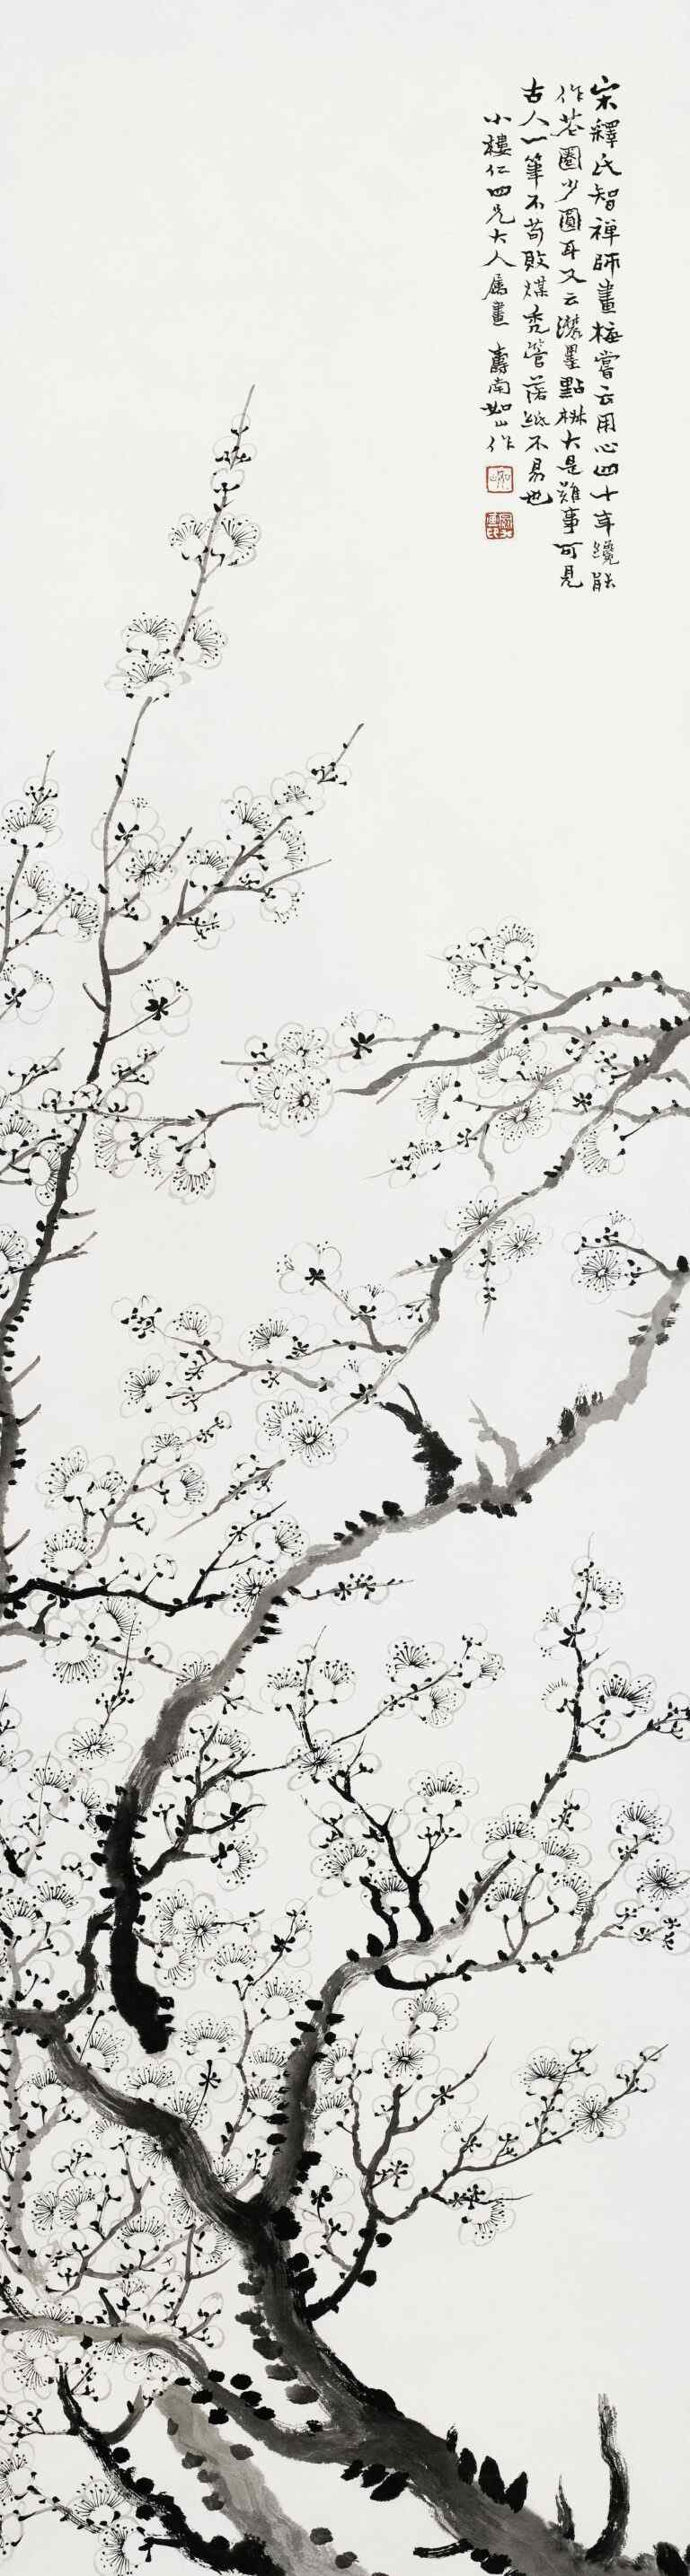
\includegraphics{../img/image07.jpg}

\begin{verseblock}

\newpage

\begin{center}\textbf{31.}\end{center}

大 道 體 寛 無 易 無 難

Dà dào tĭ kuān wú yì wú nán

El Dharma lo abarca todo,\\
no es fácil ni difícil.

\end{verseblock}

\hfill\break

\hypertarget{comentario-30}{%
\subsection{Comentario}\label{comentario-30}}

En nuestra vida cotidiana, solemos buscar lo que nos resulta más fácil y
evitar lo que percibimos como difícil. Esta tendencia puede llevarnos a
una visión superficial de la realidad, clasificando las experiencias
según nuestra comodidad o incomodidad. Sin embargo, la noción de fácil y
difícil es solo una construcción mental, una etiqueta subjetiva que
nuestra mente proyecta sobre las circunstancias.

La mente conceptual tiende a dividir el mundo en opuestos y luego se
aferra a esas categorías como si fueran verdades absolutas. Fácil y
difícil no son cualidades inherentes a la realidad, sino
interpretaciones condicionadas por nuestras expectativas, deseos y
experiencias previas. En su origen, estas distinciones surgieron como
herramientas funcionales para orientarnos en el mundo, pero con el
tiempo las hemos convertido en barreras que limitan nuestra percepción
directa de las cosas tal como son.

Si observamos con claridad, vemos que no hay experiencias
intrínsecamente fáciles o difíciles. Lo que hoy nos resulta complicado,
con la práctica se vuelve natural; lo que ahora sentimos sencillo, en
otro contexto puede convertirse en un desafío. La dificultad o la
facilidad no están en las cosas mismas, sino en la relación que
establecemos con ellas. Liberarnos de estas fijaciones nos permite
acercarnos a la realidad con una mente más abierta y receptiva, sin
prejuicios ni resistencias.

El Dharma lo abarca todo y no se rige por nuestras categorías limitadas.
No es algo que deba ser buscado en lo que consideramos fácil ni evitado
en lo que creemos difícil. Está presente en cada instante, más allá de
los juicios que proyectamos sobre él. Cultivar una mente flexible nos
permite abrazar cada experiencia con ecuanimidad, sin rechazar ni
aferrarnos, sin caer en la trampa de medir la vida en términos de
esfuerzo o comodidad.

¿Cómo acceder a este Dharma que lo abarca todo? Regresando a nuestra
condición natural, más allá de la dualidad de los conceptos, a través de
zazen. En la quietud de la práctica, la mente deja de fragmentar la
realidad y simplemente se asienta en lo que es, sin buscar lo fácil ni
rechazar lo difícil. Allí, lo que parecía distante se vuelve inmediato,
y lo que parecía inaccesible se revela como siempre presente.

\hfill\break

\hypertarget{02}{}
\begin{verseblock}

\newpage

\begin{center}\textbf{32.}\end{center}

小 見 狐 疑 轉 急 轉 遲

Xiăo jiàn hú yí zhuàn jí zhuàn chí

La visión limitada, la duda y la desconfianza;\\
Generan unas veces indecisión y otras apresuramiento.

\end{verseblock}

\hfill\break

\hypertarget{comentario-31}{%
\subsection{Comentario}\label{comentario-31}}

La mente es como un huerto: si no se cultiva con atención, pronto se
llena de maleza y malas hierbas que esparcen duda y desconfianza por
doquier. Para que florezca la claridad y la sabiduría, debemos aprender
a cuidar nuestro jardín mental con constancia y discernimiento.

Es fundamental mantenernos atentos y despiertos, evitando que la mente
sea arrastrada por la ideación descontrolada. Al igual que en un huerto
descuidado la maleza crece sin límites, una mente dejada a la deriva se
ve invadida por pensamientos dispersos y emociones reactivas. La
paciencia y la reflexión son herramientas esenciales para este cultivo
interno. Como dice el refrán: ``Vísteme despacio que tengo
prisa''---actuar sin apresurarnos, con conciencia y equilibrio, nos
permite ver con mayor claridad.

En la vida cotidiana, nuestras mentes suelen estar ocupadas por
preocupaciones superficiales y distracciones que nos alejan de una
comprensión más profunda de la realidad. En lugar de perdernos en
pensamientos limitantes, podemos aprender a enraizarnos en el momento
presente, a despejar la confusión y a abrirnos a una visión más amplia e
interconectada. Se trata, en última instancia, de reconectar con la
totalidad, con lo que realmente somos más allá de nuestras narrativas
habituales.

Por ello, cultivemos la claridad mental y eliminemos los patrones
perjudiciales, del mismo modo que arrancamos las malas hierbas de un
huerto. En un mundo cada vez más distraído, ajetreado y fragmentado,
mantener una mente lúcida y en sintonía con la realidad no solo es un
acto de bienestar personal, sino también un regalo para quienes nos
rodean. La atención plena, el discernimiento y la presencia son semillas
que, bien cuidadas, pueden transformar nuestra vida y la de los demás.

\hfill\break

\hypertarget{03}{}
\begin{verseblock}

\newpage

\begin{center}\textbf{33.}\end{center}

執 之 失 度 必 入 邪 路

Zhí zhī shī dù bì rù xié lù

Si te aferras, pierdes la ecuanimidad,\\
e inevitablemente te desvías del camino.

\end{verseblock}

\hfill\break

\hypertarget{comentario-32}{%
\subsection{Comentario}\label{comentario-32}}

En los practicantes de la Vía, y de cualquier camino espiritual, existe
el peligro de caer en el extremismo al apegarnos a las enseñanzas,
literalmente, ciegamente. La tradición Zen se ha cuidado mucho de no
caer en esta trampa y son numerosas las historias de maestros zen que
utilizan el humor y la simplicidad para contrarrestar este peligro. El
maestro Joshu, Zhaozhou Congshen (778-897), hace gala de esta
simplicidad en la siguiente historia:

En cierta ocasión, un estudiante se acercó al maestro Joshu y le
preguntó: ``Maestro, ¿puedes enseñarme el Zen?'' El maestro Joshu, un
hombre de pocas palabras, respondió con otra pregunta: ``¿Has comido tu
arroz?'' El estudiante, desconcertado por la respuesta, dijo: ``Sí, lo
he hecho''. A lo que Joshu respondió: ``Entonces, lava tu cuenco''.

La Vía no se puede atrapar con palabras ni con construcciones
conceptuales; va más allá de las explicaciones intelectuales. No es algo
que se encuentre en abstracciones elevadas, sino que se revela en la
práctica directa, en la experiencia cotidiana, en la simplicidad del
momento presente. La respuesta de Joshu es un recordatorio de que la
sabiduría no está separada de la vida diaria: se encuentra en cada acto
consciente, en la totalidad de la experiencia de cada instante.
Comprender esto no es un ejercicio teórico, sino algo que solo puede
realizarse a través de la práctica viva y la experiencia directa, libres
de apego.

Cuando nos aferramos, ya sea a conceptos, creencias o emociones,
levantamos una barrera que nos separa de la realidad tal como es.
Despertar significa darnos cuenta, una y otra vez, de cómo nos
aferramos, y soltar. La realidad no está fragmentada en sujeto y objeto;
es un todo indivisible. Cualquier apego es un signo de que seguimos
atrapados en una visión ilusoria.

El apego no se limita a los objetos materiales, sino que también puede
manifestarse en nuestra forma de pensar o en nuestra carga emocional.
Cuanto mayor es el apego, mayor es la tensión que se refleja en nuestro
cuerpo. Cuando estamos preocupados, nuestros músculos se tensan sin que
nos demos cuenta. La práctica del zen no es la causa de este dolor;
zazen nos ayuda a darnos cuenta de la tensión que ya llevamos con
nosotros, una tensión que, por cotidiana, suele pasar desapercibida.

Durante la práctica, cuando sentimos dolor en las piernas, la espalda o
el pecho, esa sensación no proviene únicamente de la postura de
meditación, sino de una tensión muscular acumulada que hemos
naturalizado a lo largo del tiempo. Dependiendo de nuestros
aferramientos, el cuerpo expresa esa carga en diferentes zonas. Tomar
conciencia de ello es el primer paso hacia la liberación. Solo cuando
nos damos cuenta del peso que hemos estado cargando podemos comenzar a
soltarlo.

\hfill\break

\hypertarget{04}{}
\begin{verseblock}

\newpage

\begin{center}\textbf{34.}\end{center}

放 之 自 然 體 無 去 住

Fàng zhī zì rán tĭ wú qù zhù

Si lo sueltas, vuelve a su propia naturaleza,\\
su esencia no va ni viene.

\end{verseblock}

\hfill\break

\hypertarget{comentario-33}{%
\subsection{Comentario}\label{comentario-33}}

Soltar significa permitir que la mente siga su curso natural, sin
aferrarnos a sus contenidos, ya sean pensamientos, emociones, deseos o
miedos incesantes. En la meditación zen, observamos la mente sin juicio
ni apego, con ecuanimidad, dejando que los pensamientos surjan y
desaparezcan sin intervenir, como si nuestra conciencia fuera un espejo
que refleja todo lo que aparece instante tras instante. Al permitir que
la mente fluya según su propia naturaleza, nos liberamos del sufrimiento
que surge del aferramiento. Se trata de comprender que «lo que es, es»,
aceptando la realidad tal como se presenta, sin resistencia ni rechazo.

La verdadera naturaleza de la mente es intrínsecamente estable. Aunque
en la superficie la mente esté en constante movimiento, existe una
quietud subyacente que se revela de forma natural cuando practicamos
zazen. Esta quietud es como el fondo del océano: profundo, sereno,
inmutable. Sin embargo, solemos identificarnos con las olas ---los
pensamientos, emociones y fluctuaciones mentales--- olvidando la
vastedad del océano que realmente somos. Como dice el maestro Eihei
Dōgen (1200-1254) en el Bendōwa: «Debes comprender que nadie carece de
la insuperable Conciencia Despierta y que ya vives siempre en su
plenitud, pero no te das cuenta de ello.»

Esta naturaleza fundamental no es una entidad fija ni una sustancia que
pueda ser definida. Es pura vacuidad, más allá del alcance del
intelecto. No puede ser categorizada como ``móvil'' o ``estática'',
``ancha'' o ``estrecha'', ya que trasciende todas las dualidades y las
concepciones limitadas de la mente humana. Nuestra práctica consiste en
reconocer la tranquilidad intrínseca que subyace a todo el flujo de
pensamientos y percepciones.

En el fondo, todos anhelamos esta serenidad, porque es nuestro verdadero
hogar. Zazen es la puerta de entrada principal a este reconocimiento, el
retorno a lo que siempre ha estado aquí, más allá de toda
conceptualización, simplemente siendo.

\hfill\break

\hypertarget{05}{}
\begin{verseblock}

\newpage

\begin{center}\textbf{35.}\end{center}

任 性 合 道 逍 遙 絶 惱

Rèn xìng hé dào xiāo yáo jué năo

Cuando confiamos en la naturaleza de las cosas,\\
hay armonía y se extinguen las aflicciones.

\end{verseblock}

\hfill\break

\hypertarget{comentario-34}{%
\subsection{Comentario}\label{comentario-34}}

En el zen, confiar en la naturaleza de las cosas implica una aceptación
profunda de la realidad tal como es, sin aferrarnos ni rechazarla, sin
quedar atrapados en los extremos. Estar en armonía con la esencia
fundamental de la existencia es el corazón de la práctica. Esta
confianza no es una actitud pasiva, sino una forma de vivir con
autenticidad, alineándonos con la verdad en cada instante de conciencia.

Una de las manifestaciones más claras de esta confianza es la paciencia,
la capacidad de observar las situaciones con la perspectiva adecuada,
sin dejarnos arrastrar por reacciones impulsivas ni juicios apresurados.
Confiamos en que la realidad se despliega conforme a su propia
naturaleza y en que, con una mente serena, podemos afrontarla con
sabiduría. No se trata de resignación, sino de una apertura genuina a lo
que es, sin imponerle nuestras expectativas.

Esta actitud nos libera del peso de las preocupaciones innecesarias, de
las cargas mentales y emocionales que a menudo generan sufrimiento. La
práctica del desapego y la aceptación juega un papel esencial en este
proceso, permitiéndonos experimentar la vida con mayor ligereza y
claridad. No significa ignorar los desafíos, sino abordarlos con una
mente equilibrada y ecuánime, sin la ansiedad de querer controlarlo
todo.

En una época donde el estrés y la ansiedad han alcanzado niveles
críticos, esta perspectiva nos recuerda la importancia de confiar en la
naturaleza intrínseca de las cosas, fluir con la vida y experimentar la
libertad de soltar lo que no necesitamos. Vivir con sencillez, en
conexión con la naturaleza y con el presente, dejando atrás la obsesión
por el control y el éxito. Abrazar la incertidumbre y la impermanencia
con naturalidad, en lugar de luchar contra ellas.

Cuando nos identificamos por completo con las circunstancias que nos
rodean, sin la distancia necesaria, nuestra percepción se distorsiona.
La identificación ciega nos impide ver las cosas como realmente son:
interconectadas, armoniosas y libres en su esencia. Nos aferramos a
nuestras interpretaciones limitadas, generando sufrimiento innecesario.
Al soltar esta identificación rígida y cultivar la paciencia, podemos
abrirnos a una comprensión más profunda: la realidad, no es una amenaza
a la que debamos resistirnos, sino un flujo natural que podemos aprender
a habitar con confianza y serenidad.

\hfill\break

\begin{center}\rule{0.5\linewidth}{0.5pt}\end{center}

\hfill\break

\hypertarget{01}{}
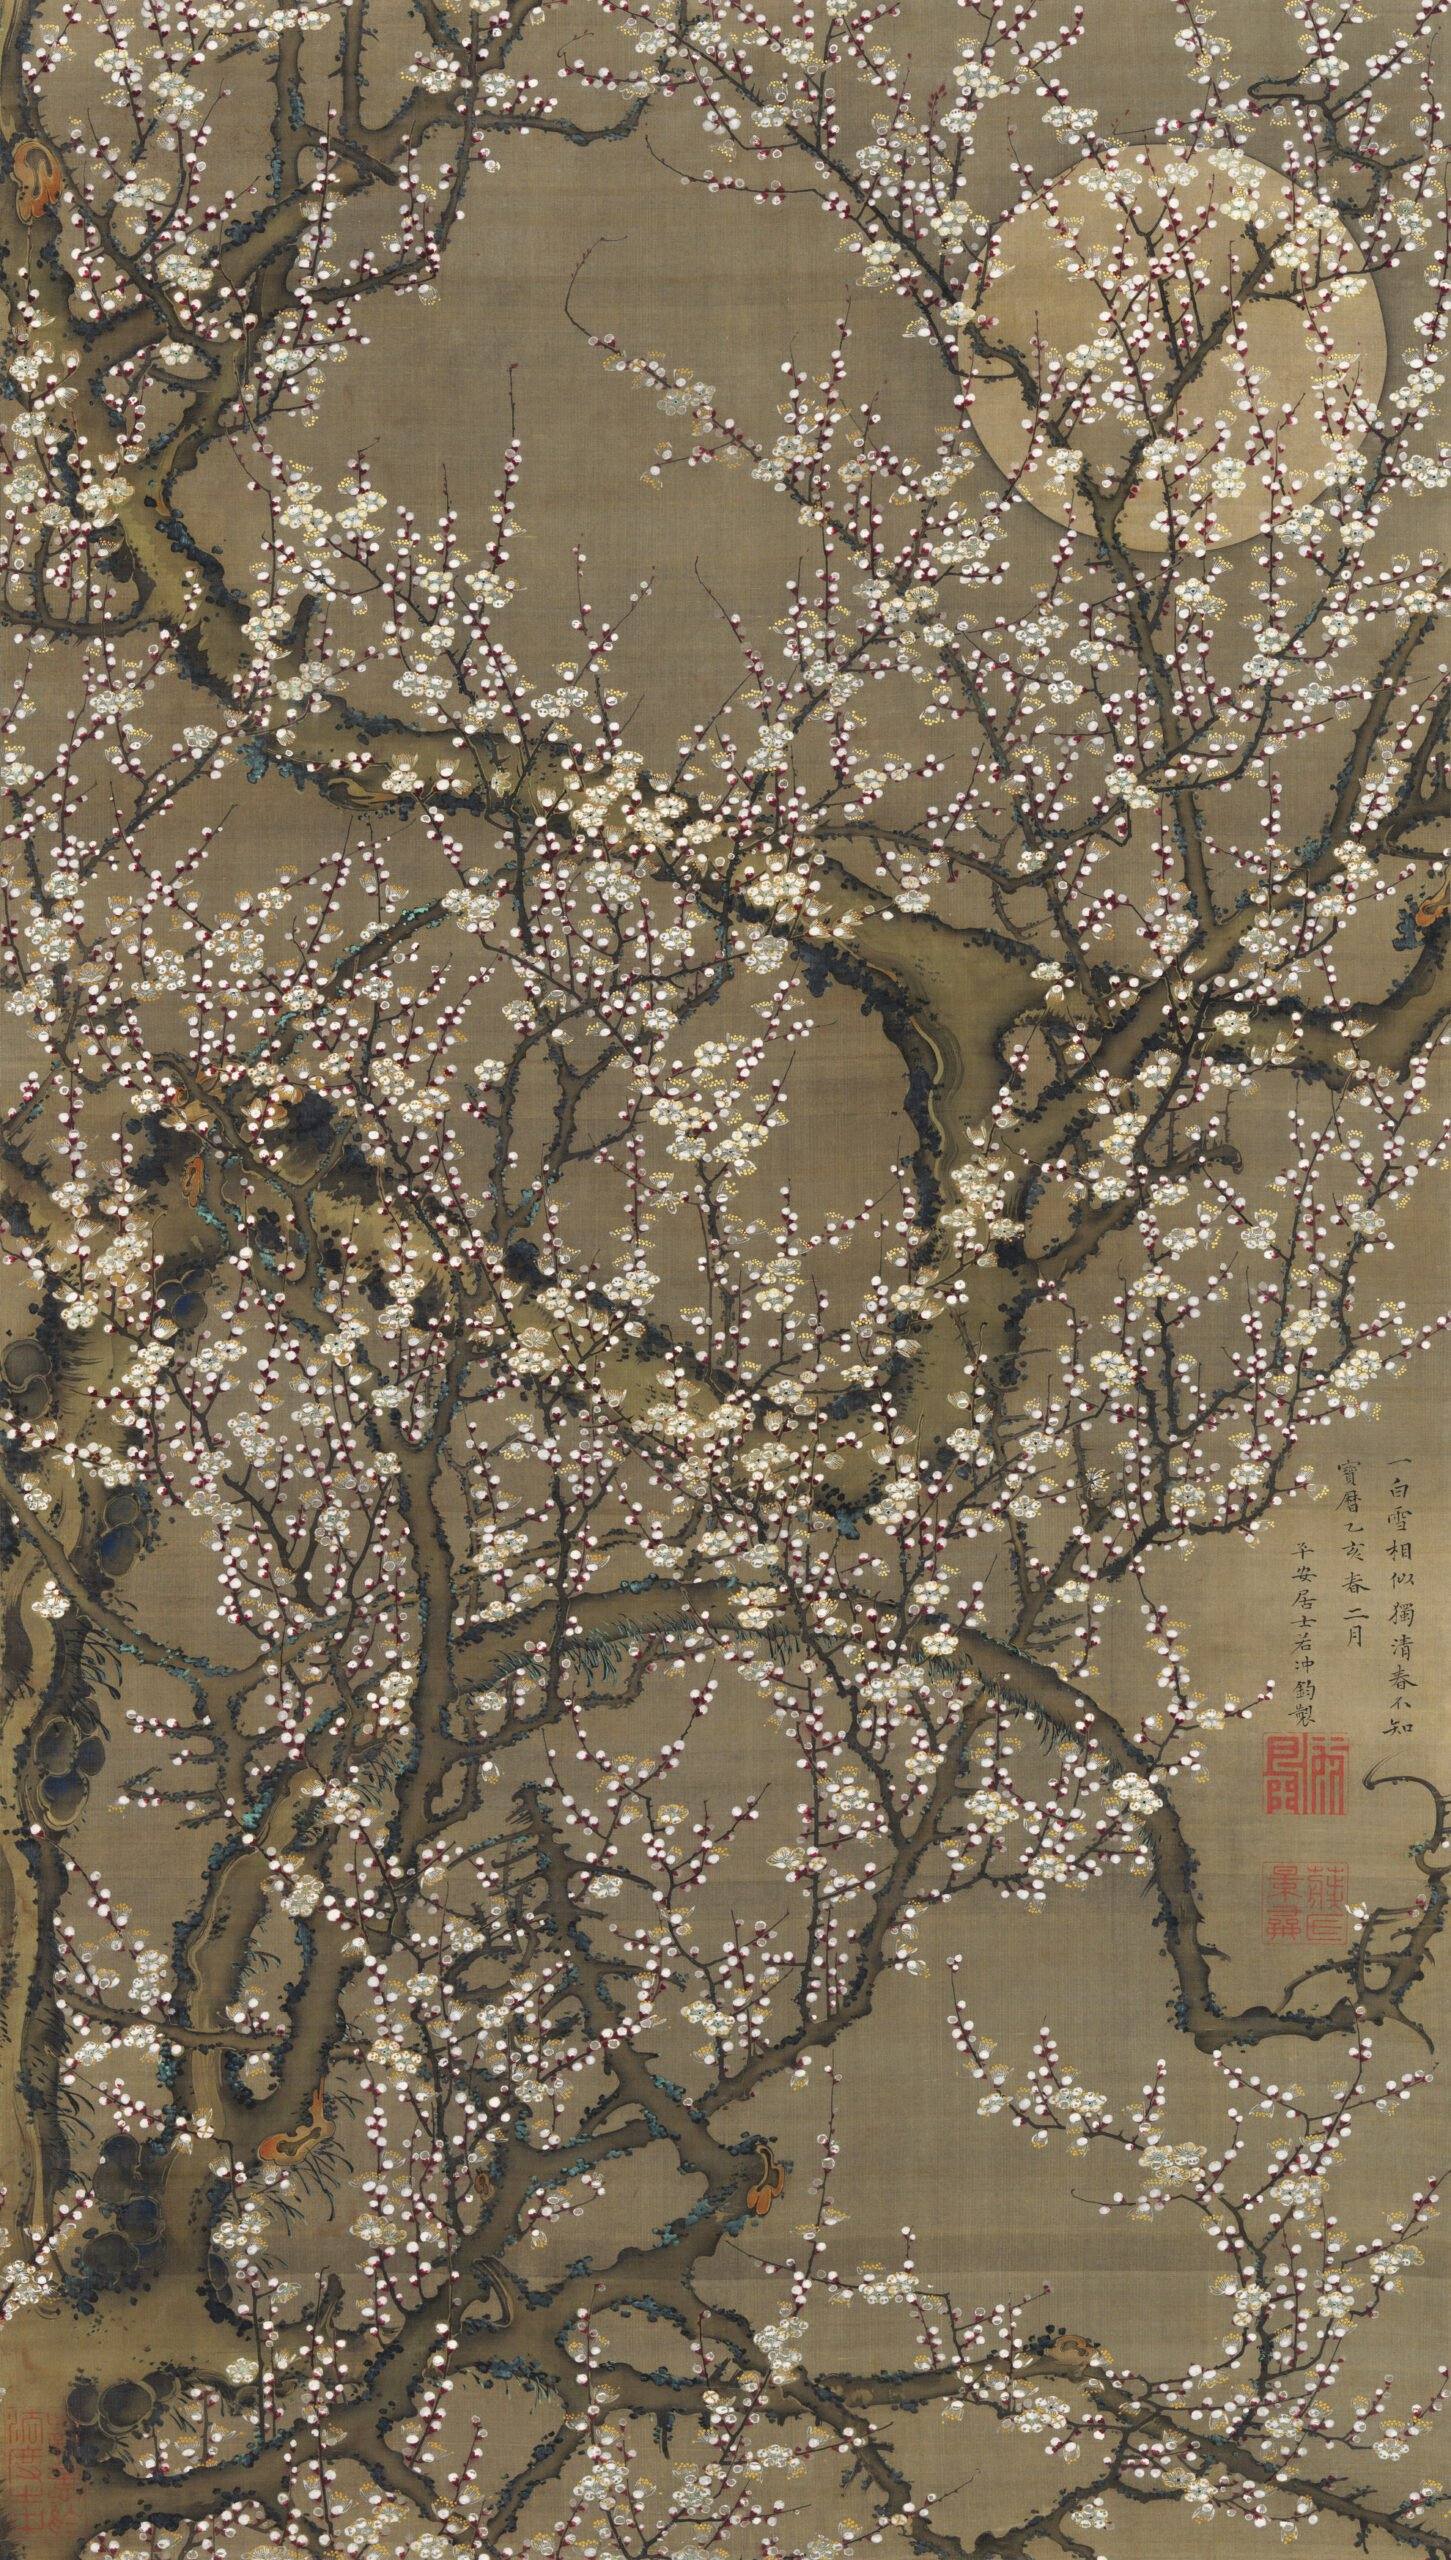
\includegraphics{../img/image08.jpg}

\begin{verseblock}

\newpage

\begin{center}\textbf{36.}\end{center}

繋 念 乖 眞 昏 沈 不 好

Xì niàn guāi zhēn hūn chén bù hăo

Aferrarse a los pensamientos nos aleja de la realidad,\\
la mente se oscurece y se hunde en lo indeseable.

\end{verseblock}

\hfill\break

\hypertarget{comentario-35}{%
\subsection{Comentario}\label{comentario-35}}

El pensamiento nos permite interpretar y comprender el mundo que nos
rodea. Al mismo tiempo, no es la realidad en sí misma, sino una
representación filtrada y subjetiva de ella. Cuando nos identificamos
demasiado con nuestros pensamientos, nos desconectamos tanto de la
realidad como de nuestra verdadera naturaleza. Aferrarse a los
pensamientos nos aleja de la realidad porque nos encierra en una versión
limitada del mundo, una proyección de nuestras memorias, deseos y
temores.

En lugar de experimentar directamente, interpretamos y juzgamos,
generando una separación artificial entre nosotros y la vida tal como
es. La mente humana construye narrativas, interpretaciones y juicios
constantes sobre lo que experimentamos. Al identificarnos con estos
pensamientos, percibimos la realidad a través de un prisma distorsionado
por nuestras experiencias, creencias y emociones. En vez de ver la
totalidad de lo que es, nos quedamos con una versión limitada y parcial.

A pesar de ello, el pensamiento es una herramienta valiosa cuando lo
usamos con discernimiento. En lugar de ser arrastrados por él, podemos
aprender a observarlo con claridad, dándonos cuenta de que no somos
nuestros pensamientos. Esta capacidad de distanciamiento nos permite
utilizarlos de manera funcional para analizar, planificar y comprender
sin caer en la ilusión de que nuestras interpretaciones son la verdad
absoluta.

La práctica de zazen nos ofrece un medio directo para desarrollar esta
relación saludable con el pensamiento. Al cultivar la conciencia plena,
aprendemos a observar el flujo mental sin quedar atrapados en él. Esta
distancia nos permite experimentar la realidad con mayor claridad, sin
las distorsiones impuestas por nuestros juicios automáticos.

Uno de los principios fundamentales en la enseñanza budista es encontrar
el equilibrio entre los extremos. En la práctica de la meditación zen,
el exceso de actividad mental se conoce como Sanran, un estado
caracterizado por una mente agitada y un cuerpo tenso. En este estado,
surgen innumerables pensamientos, recuerdos, deseos y sensaciones.
Corporalmente, la barbilla se eleva, los pulgares se crispan y los
músculos se contraen. Es la actitud típica de quienes "piensan"
demasiado durante zazen. Por el contrario, la falta de claridad mental
en la meditación se denomina Kontin, un estado de somnolencia en el que
la vigilancia disminuye y el tono muscular se debilita. Aquí, la
atención se disuelve, la postura se desploma, la cabeza cae hacia
adelante y las manos pierden vigor.

¿Cómo armonizar estos extremos y encontrar el equilibrio? Zazen es un
espejo que nos permite percibir con claridad cuándo nuestra conciencia
está desequilibrada y necesita ser reajustada. Perseverar en la práctica
es esencial para reconocer las causas de estos estados y comprender cómo
influyen en nuestra vida cotidiana. Cuando la mente no oscila entre la
dispersión y la inercia, emerge una claridad natural. En ese estado de
presencia, la realidad se muestra tal como es, sin los filtros del
juicio, ni la distorsión del apego o el rechazo. Zazen nos enseña a
habitar plenamente cada instante y a encontrar en la simplicidad del
ahora la expresión más profunda del despertar.

\hfill\break

\hypertarget{02}{}
\begin{verseblock}

\newpage

\begin{center}\textbf{37.}\end{center}

不 好 勞 神 何 用 疏 親

Bù hăo láo shén Hé yòng shū qīn

No es bueno agotar la energía vital,\\
¿Para qué huir, para qué seguir buscando?

\end{verseblock}

\hfill\break

\hypertarget{comentario-36}{%
\subsection{Comentario}\label{comentario-36}}

Frecuentemente, nos sumergimos en la vorágine de nuestras preocupaciones
sin detenernos a considerar en qué dirección estamos dirigiendo nuestra
energía vital. ¿Cómo y en qué la invertimos? Esta energía es un recurso
precioso y limitado, y sin darnos cuenta, la gastamos en preocupaciones
innecesarias, en resistencias y apegos que nos consumen sin aportar
verdadero valor a nuestras vidas. ¿Cuántas veces nos aferramos a aquello
que solo nos desgasta? ¿Cuántas veces intentamos huir de lo desagradable
sin darnos cuenta de que, en ese intento de escape, estamos
desperdiciando una energía que podríamos emplear de manera más sabia en
nuestro bienestar y en el de quienes nos rodean?

Pero, ¿acaso esta búsqueda constante nos lleva realmente a algún lugar?
¿No es, en sí misma, una forma de agotamiento, de dispersión? No es
necesario agotar nuestra energía en una lucha sin fin, en el anhelo de
algo que creemos que nos falta o en el temor a lo que nos persigue.
Cuando dejamos de correr, cuando soltamos la necesidad de escapar o de
encontrar respuestas en otra parte, descubrimos que la plenitud no está
en el futuro ni en otro lugar: siempre ha estado aquí.

Tomar conciencia de nuestra energía vital implica estar plenamente
presentes, reconocer nuestras elecciones y dirigir nuestra atención
hacia lo que verdaderamente importa. Por eso, es fundamental hacer una
pausa, sentarnos y sentirnos, observarnos y conectar con lo que
realmente tiene valor en este instante, dentro de las circunstancias que
estamos viviendo.

La práctica de la meditación Zen nos ofrece una herramienta invaluable
para cultivar esta conciencia. Al entrenar la mente para habitar el
momento presente, aprendemos a soltar las preocupaciones superfluas y a
enfrentar lo desagradable con ecuanimidad. La meditación no es solo un
acto de quietud durante zazen, sino un entrenamiento continuo que se
extiende a la vida cotidiana, guiándonos hacia una gestión más sabia de
nuestra energía vital.

No busquemos más. No nos desgastemos en la huida. Soltar no es perder,
sino reencontrarnos con lo que siempre ha estado en nosotros. En la
simplicidad del instante presente, en la respiración que entra y sale
sin esfuerzo, hallamos la paz que nunca nos ha abandonado.

No agotemos nuestra energía en vano. No nos dejemos atrapar por apegos
innecesarios ni por la inercia del pensamiento obsesivo. Que la
conciencia sea nuestra brújula, permitiéndonos dirigir nuestra energía
hacia lo que realmente importa. En cada respiración y en cada elección,
encontramos la oportunidad de vivir con mayor plenitud y consciencia.

\hfill\break

\hypertarget{03}{}
\begin{verseblock}

\newpage

\begin{center}\textbf{38.}\end{center}

欲 取 一 乘 勿 惡 六 塵

Yù qŭ yī chéng wù è liù chén

Si deseas alcanzar el Gran Despertar,\\
no rechaces las seis sensaciones.

\end{verseblock}

\hfill\break

\hypertarget{comentario-37}{%
\subsection{Comentario}\label{comentario-37}}

En la tradición budista, las seis clases de sensaciones abarcan las
experiencias que surgen a través de los órganos de los sentidos: la
vista, el oído, el olfato, el gusto, el tacto y la mente.

A diferencia de la concepción occidental, que limita la percepción a los
cinco sentidos físicos, el budismo reconoce a la mente (manas) como un
sexto sentido. Esto se debe a que la mente no solo procesa información,
sino que también percibe objetos mentales, como pensamientos, recuerdos
e imágenes internas, de la misma manera que los ojos perciben formas o
los oídos perciben sonidos. Así, al igual que los demás sentidos, la
mente genera experiencias que pueden ser placenteras, desagradables o
neutras, y que pueden dar lugar a apego o aversión.

No debemos caer en los extremos del rechazo o el apego a estas
sensaciones. El Buda histórico, Siddhartha Gautama, experimentó ambos
extremos antes de alcanzar el despertar. Practicó el ascetismo,
renunciando a toda comodidad y buscando la liberación a través de la
privación, pero comprendió que este enfoque no conducía a la verdad
última.

Encontrar un equilibrio entre rechazo y apego es fundamental. No
rechazar las sensaciones significa no ignorar ni evitar nuestras
experiencias, ya sean externas o internas, pues son parte de la vida y
pueden enseñarnos algo valioso. Pero tampoco debemos caer en el apego,
permitiendo que las sensaciones nos arrastren y dicten nuestras
emociones y acciones. Esto se aplica tanto a las percepciones físicas
como a los pensamientos y emociones que surgen en la mente.

Este equilibrio nos permite desarrollar una comprensión más profunda de
la realidad. Cuando observamos con ecuanimidad las experiencias
sensoriales y los fenómenos mentales sin aferrarnos ni rechazarlos,
podemos liberar la mente de sus ataduras y acercarnos a una experiencia
más directa y auténtica.

\hfill\break

\hypertarget{04}{}
\begin{verseblock}

\newpage

\begin{center}\textbf{39.}\end{center}

六 塵 不 惡 還 同 正 覺

Liù chén bù è hái tóng zhèng jué

Cuando no se rechazan las seis sensaciones,\\
se alcanza el auténtico despertar.

\end{verseblock}

\hfill\break

\hypertarget{comentario-38}{%
\subsection{Comentario}\label{comentario-38}}

Cuando nuestra mente está libre de apegos y aversiones, podemos percibir
los seis sentidos como lo que realmente son: vacíos de existencia
inherente. No hay un "yo" separado que perciba ni objetos con una
esencia propia que sean percibidos. En este estado de apertura, los seis
sentidos se experimentan sin la distorsión de nuestras proyecciones y
condicionamientos. Así, los sentidos dejan de ser fuente de ilusión y
sufrimiento y se revelan como expresión de la budeidad, el estado de
despertar.

La budeidad no es una realidad separada de nuestra experiencia
cotidiana, sino la comprensión directa de la interdependencia de todos
los fenómenos. En el estado de despertar, dejamos de estar atrapados en
el samsara, no porque los fenómenos desaparezcan, sino porque cesa
nuestra fijación en ellos. Podemos experimentar la realidad tal como es,
sin el velo de nuestras preferencias y rechazos.

Los fenómenos que nos rodean no son intrínsecamente buenos o malos; son
simplemente lo que son. Es nuestra mente, condicionada por el apego y la
aversión, la que proyecta juicios y genera sufrimiento. Cuando logramos
liberar la mente de estas distorsiones, podemos ver la realidad con
claridad, en toda su plenitud y perfección. La belleza de la existencia
no radica en la ausencia de dificultades, sino en nuestra capacidad para
experimentarlas sin resistencia, en la aceptación profunda de lo que es.

La puerta de entrada a este estado es la práctica de zazen. En la
postura sedente, inmóviles, enfocando la atención en el cuerpo y la
respiración sin perseguir beneficio alguno, accedemos de manera natural
a un estado ecuánime, libre de apego y rechazo. En zazen, no buscamos
alcanzar un estado especial ni escapar de la realidad, sino simplemente
asentarnos en el momento presente, dejando que la mente repose en su
claridad original. Este equilibrio, que no es forzado ni fabricado,
surge de la quietud y la observación profunda.

Es fundamental comprender que el perfecto despertar no es un ideal
lejano ni un logro reservado a unos pocos. No es algo externo a
nosotros, sino nuestra naturaleza más profunda, de la cual nos hemos
desconectado debido a la ignorancia y los hábitos condicionados. La
práctica de zazen no nos da algo nuevo, sino que nos permite regresar a
lo que siempre ha estado ahí: la presencia serena, la mente sin
obstrucciones.

\hfill\break

\hypertarget{05}{}
\begin{verseblock}

\newpage

\begin{center}\textbf{40.}\end{center}

智 者 無 爲 愚 人 自 縛

Zhì zhě wú wéi Yú rén zì fú

El sabio no actúa forzadamente.\\
El ignorante se ata a sí mismo.

\end{verseblock}

\hfill\break

\hypertarget{comentario-39}{%
\subsection{Comentario}\label{comentario-39}}

El sabio, en su profunda comprensión, sabe que la verdadera acción no
siempre implica un hacer constante. La realidad, tal como se manifiesta,
es intrínsecamente perfecta. Desde nuestra perspectiva limitada,
percibimos carencias y defectos: anhelamos ser más delgados, más altos,
más inteligentes, más asertivos o que no haya guerras ni injusticias.
Sin embargo, desde la mente despierta, la realidad ya es completa y se
sostiene en un equilibrio perfecto, más allá de nuestros juicios y
expectativas.

Nuestra percepción parcial nos hace creer que algo nos falta, que
siempre hay una mejora posible. Esta búsqueda incesante de superación
personal es agotadora y nos aleja de la plenitud del momento presente.
Desde una mirada más ecuánime, la realidad se despliega como un tapiz
perfecto, donde incluso las imperfecciones aparentes forman parte de su
naturaleza intrínseca.

Un anciano sabio vivía en un pequeño pueblo y poseía un hermoso caballo.
Un día, el caballo escapó. Los vecinos acudieron a consolarlo diciendo:
"¡Qué desgracia! Has perdido tu único caballo." Pero el anciano
respondió con calma: "¿Buena suerte? ¿Mala suerte? ¿Quién sabe?"

Días después, el caballo regresó trayendo consigo una manada de caballos
salvajes. Los vecinos, sorprendidos, exclamaron: "¡Qué buena fortuna!
Ahora tienes más caballos." El anciano solo respondió: "¿Buena suerte?
¿Mala suerte? ¿Quién sabe?"

Poco después, el hijo del anciano intentó domar uno de los caballos
salvajes, pero cayó y se rompió una pierna. Los vecinos dijeron: "¡Qué
desgracia! Ahora tu hijo está herido y no puede trabajar." Pero el
anciano repitió: "¿Buena suerte? ¿Mala suerte? ¿Quién sabe?"

Semanas después, el ejército del rey llegó al pueblo reclutando jóvenes
para la guerra. Todos los jóvenes fueron llevados, excepto el hijo del
anciano, que no pudo ser reclutado debido a su pierna rota. "¡Qué gran
suerte!" dijeron los vecinos. El anciano, una vez más, respondió:
"¿Buena suerte? ¿Mala suerte? ¿Quién sabe?"

No es fácil aceptar la existencia de guerras, pandemias y sufrimiento.
Nos parece contradictorio pensar que, desde una perspectiva más amplia,
todo está bien. Aquí es donde la sabiduría de la práctica se vuelve
esencial: necesitamos la capacidad de ver más allá de nuestras
percepciones condicionadas y comprender que todo lo que ocurre forma
parte de un orden mayor, aunque escape a nuestra comprensión inmediata.

¿Cómo perciben las estrellas nuestro deseo de ser más delgados, más
inteligentes o más exitosos? La naturaleza misma no busca la perfección
en esos términos. El río fluye sin preocuparse por si su cauce es recto
o sinuoso, las montañas no se lamentan por su altura ni los árboles por
la forma de sus ramas. La verdadera liberación no se encuentra en
transformar lo que somos o en imponer un orden a la existencia, sino en
aceptarnos sin condiciones, tal como la vida se presenta en este
momento.

Sentarse, sentirse y sumergirse en la autoaceptación son pasos
fundamentales para liberarnos de las expectativas y los estándares
autoimpuestos. Al cocernos en nuestra propia salsa, nos permitimos
aceptar lo que somos sin juicios ni exigencias y abrirnos a la realidad
tal como es. En esta aceptación incondicional, la inquietud por ser más
se disuelve y, en su lugar, emerge la serenidad. Al dejar de luchar
contra lo que es, descubrimos que la verdadera libertad no radica en
transformarnos, sino en despertar a nuestra naturaleza original, que
siempre ha estado ahí.

\hfill\break

\hfill\break

\hypertarget{01}{}
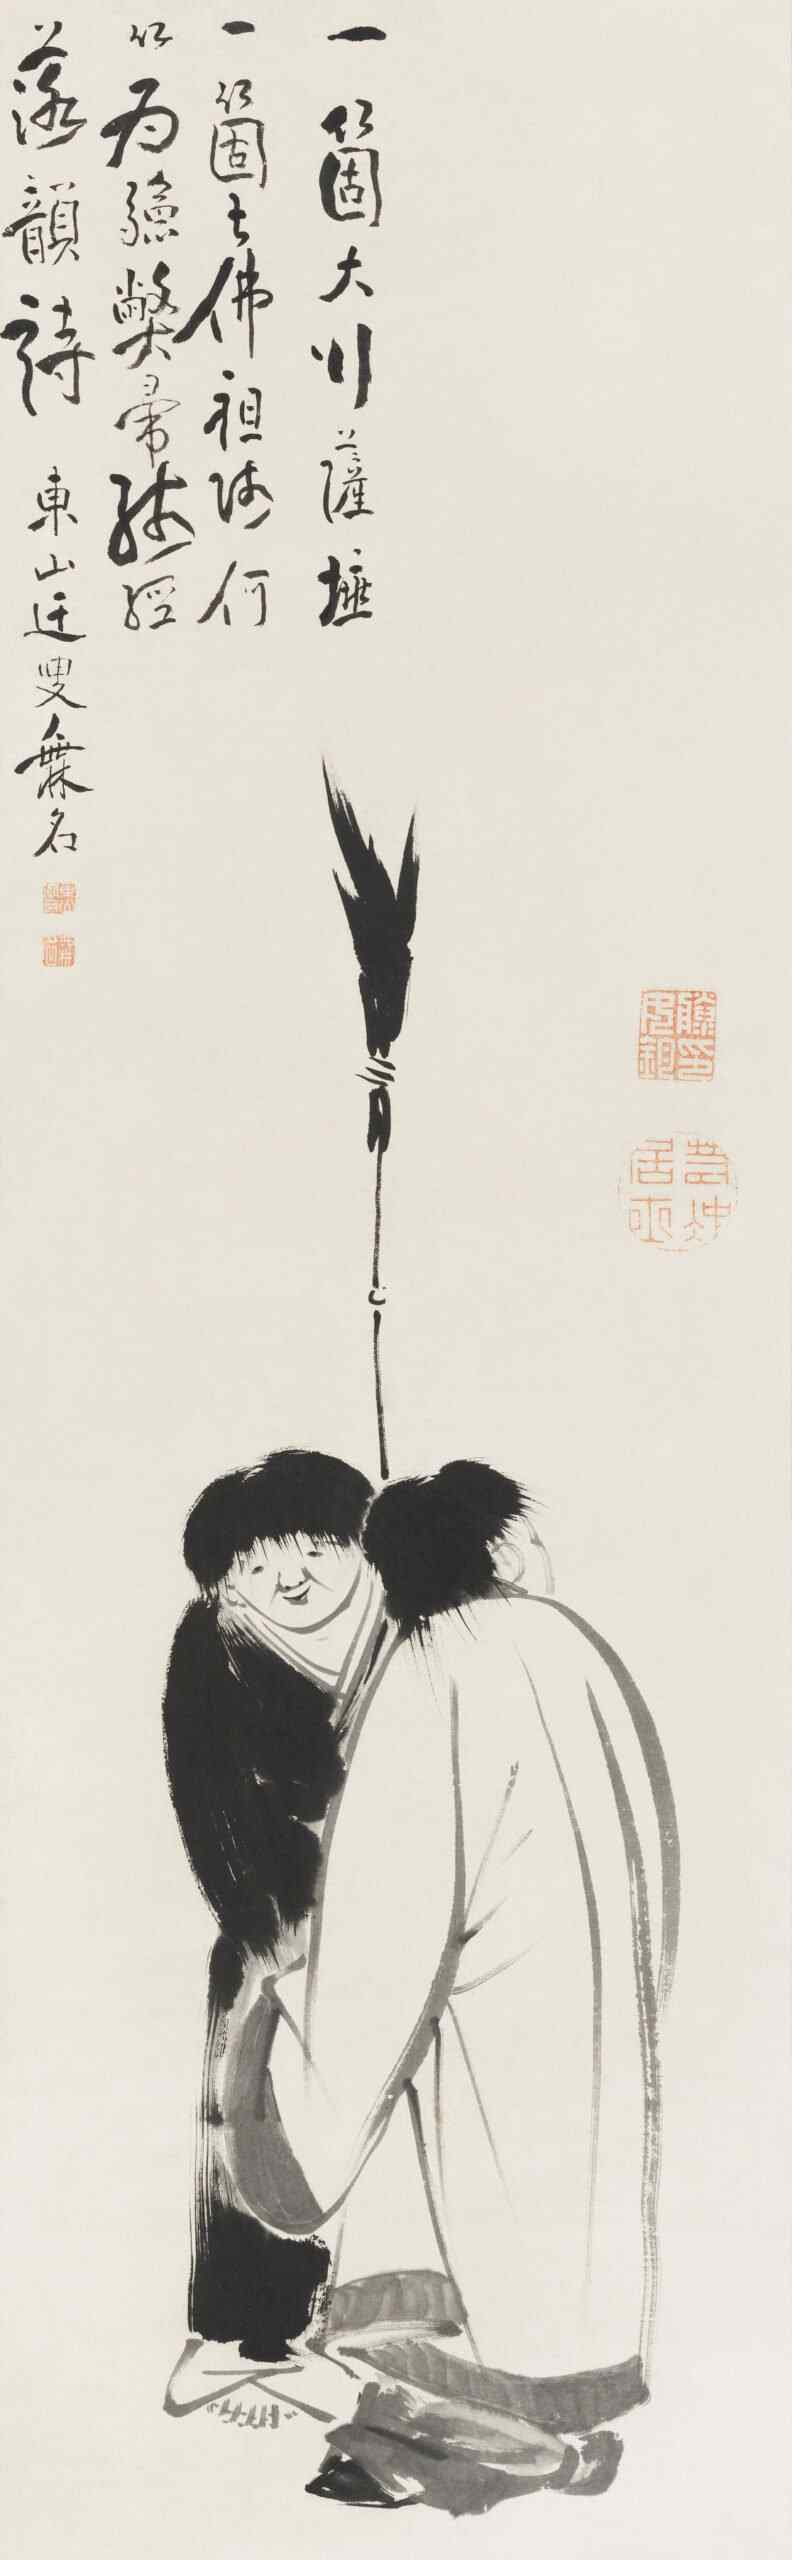
\includegraphics{../img/image09.jpg}

\begin{verseblock}

\newpage

\begin{center}\textbf{41.}\end{center}

法 無 異 法 妄 自 愛 著

Fă wú yì fă Wàng zì ài zhù

El Dharma está más allá de la dualidad,\\
pero los ilusos lo convierten en objeto de apego.

\end{verseblock}

\hfill\break

\hypertarget{comentario-40}{%
\subsection{Comentario}\label{comentario-40}}

Los fenómenos, en su esencia, no son diferentes entre sí; es nuestra
mente, atrapada en el apego, la que genera la ilusión de separación. La
realidad se manifiesta como un todo interconectado, pero nuestras
preferencias, aversiones y juicios la fragmentan, haciéndonos creer en
diferencias sustanciales donde en verdad solo hay unidad.

Los tres venenos ---apego, aversión e indiferencia--- condicionan
nuestra percepción y nos mantienen atrapados en la dualidad. El apego
nos aferra a lo que consideramos deseable, generando miedo a la pérdida.
La aversión nos empuja a rechazar lo que nos resulta incómodo,
negándonos la oportunidad de verlo con claridad. La indiferencia nos
insensibiliza, impidiendo que experimentemos la realidad en su
totalidad. Estos patrones nos separan de la experiencia directa, creando
la ilusión de un mundo fragmentado cuando, en realidad, todo es
expresión de una misma naturaleza.

Cultivar la ecuanimidad es trascender esta visión distorsionada. No se
trata de reprimir nuestras respuestas emocionales, sino de observarlas
sin quedarnos atrapados en ellas. Ver sin aferrarnos. Escuchar sin
rechazar. Sentir sin endurecernos. Cuando dejamos de etiquetar cada
experiencia como buena o mala, deseable o indeseable, la mente se abre a
una comprensión más profunda y directa de la realidad.

Uno de los seis paramitas del bodhisattva es la paciencia (kṣānti).
Paciencia no es una mera tolerancia pasiva ni una espera resignada, sino
una aceptación profunda de lo que es. Paciencia es permitir que la
realidad se despliegue sin imponerle nuestras expectativas. Es la
disposición a permanecer en el presente sin lucha ni resistencia,
comprendiendo que cada fenómeno surge y desaparece sin una identidad
fija. Y es, también, la perseverancia en la práctica, el compromiso de
seguir caminando el sendero del despertar con ecuanimidad y claridad.

Soltar el apego a la ilusión de diferencia nos permite descansar en la
realidad tal como es, sin necesidad de forzarla ni rechazarla.

\hfill\break

\hypertarget{02}{}
\begin{verseblock}

\newpage

\begin{center}\textbf{42.}\end{center}

將 心 用 心 豈 非 大 錯

Jiāng xīn yòng xīn qĭ fēi dà cuò

Si tratas de usar la mente para comprender la mente,\\
¿Acaso no es un gran error?

\end{verseblock}

\hfill\break

\hypertarget{comentario-41}{%
\subsection{Comentario}\label{comentario-41}}

Intentar comprender la mente con la mente misma es una paradoja. Es como
querer lavar una mancha de sangre con sangre, o intentar levantarse del
suelo tirándose del propio cabello. Este es el callejón sin salida del
autoconocimiento cuando se persigue desde los propios mecanismos
mentales. La mente, esa herramienta que nos permite percibir, pensar y
conceptualizar, se convierte al mismo tiempo en el velo que nos impide
ver más allá de sus propios límites.

Existe un camino más allá de estas fronteras autoimpuestas. Trascender
la mente no significa rechazarla, sino comprender su funcionamiento, su
tendencia a girar en bucles, a retroalimentarse. En esa comprensión
profunda ---no meramente intelectual, sino vivencial--- se encuentra la
llave para deshacer el nudo que nos ata al sufrimiento y a la ilusión
del control.

Es como abrir una puerta hacia un espacio más amplio, donde el silencio
no es vacío, sino plenitud. Al mirar desde ese lugar, ya no nos sentimos
atrapados en la narrativa interna, en las explicaciones, en la necesidad
constante de entender. Aparece entonces una forma distinta de saber:
directa, inmediata, libre.

La práctica del Zen nos conduce justamente ahí. No se trata de acumular
conceptos ni de perfeccionar teorías, sino de experimentar. Sentarse,
soltar, observar sin juicio. Ir más allá de la mente que etiqueta, que
clasifica, que se aferra. ¿Qué hay más allá del pensamiento? ¿Qué ocurre
cuando dejamos de intentar entender y simplemente somos?

Como decimos en Zen:

Si la ocasión se presenta, experiméntalo.

\hfill\break

\hypertarget{03}{}
\begin{verseblock}

\newpage

\begin{center}\textbf{43.}\end{center}

迷 生 寂 亂 悟 無 好 惡

Mí shēng jì luàn Wù wú hào wù

En la ignorancia surge la quietud y la agitación,\\
en el despertar cesan el apego y el rechazo.

\end{verseblock}

\hfill\break

\hypertarget{comentario-42}{%
\subsection{Comentario}\label{comentario-42}}

En el modo automático de existencia somos marionetas de nuestros deseos,
perseguimos incansablemente lo que anhelamos y huimos de lo que juzgamos
como desagradable, solo para encontrarnos enredados en un ciclo
interminable de aparente orden y caos. Atrapados en un juego incesante
de atracción y rechazo, como un hámster en su rueda, sin poder parar
para llegar a ninguna parte.

El despertar nos permite trascender esta dualidad. Al liberarnos de las
cadenas de la atracción y el rechazo, encontramos una paz que trasciende
las circunstancias cotidianas. Este despertar va mucho más allá de lo
que podamos encontrar en los libros, debe ser una experiencia que emane
desde las entrañas de nuestra sabiduría innata.

La ignorancia es como un estado de ensoñación, donde seguimos los
impulsos de nuestros deseos automáticamente. Pero, ¿qué sucede cuando
nos despertamos de este sueño? En el despertar, cesa la atracción y el
rechazo. Nos convertimos en observadores conscientes de la vida, capaces
de fluir con los acontecimientos en lugar de resistirnos a ellos.

La verdadera comprensión no proviene solo de lo que hemos leído o
aprendido de otros, sino de sumergirnos en las aguas de nuestra
experiencia personal. Es a través de nuestras propias vivencias que
descubrimos la verdad interna que trasciende las palabras impresas.

Forma parte de nuestra responsabilidad encontrar el camino hacia el
despertar. En lugar de depender ciegamente de las enseñanzas externas,
nos sumergimos en la riqueza de la experiencia directa. Este viaje hacia
la verdad desde dentro nos libera de la dualidad de la atracción y el
rechazo, permitiéndonos abrazar la plenitud de la vida con una mente
clara y un corazón abierto.

El despertar es un proceso continuo, una invitación constante a mirar
más allá de las apariencias y descubrir la verdad que yace en el núcleo
de nuestra existencia.

\hfill\break

\hypertarget{04}{}
\begin{verseblock}

\newpage

\begin{center}\textbf{44.}\end{center}

一 切 二 邊 良 由 斟 酌

Yī qiē èr biān liáng yóu zhēn zhuó

La existencia de los opuestos,\\
es producto de la evaluación mental.

\end{verseblock}

\hfill\break

\hypertarget{comentario-43}{%
\subsection{Comentario}\label{comentario-43}}

Los pares de opuestos ---bien y mal, placer y dolor, vida y muerte--- no
existen por sí mismos. Son construcciones mentales, etiquetas que la
mente utiliza para orientarse en el mundo. El pensamiento clasifica,
delimita, compara. Nos ofrece mapas, pero no el territorio.

Esta capacidad de discriminar tiene su función, pero cuando nos
identificamos con ella, confundimos los mapas con la realidad. Creemos
que debemos elegir siempre entre uno y otro extremo: aferrarnos al
placer y evitar el dolor, buscar la vida y negar la muerte, abrazar lo
que nos gusta y rechazar lo que nos incomoda. Así, sin darnos cuenta,
nos atrapamos en un juego de tensiones que genera conflicto y
sufrimiento.

El problema no está en el pensamiento, sino en la identificación con él.
Cuando creemos que nuestras ideas son la realidad, nos perdemos en una
visión fragmentada del mundo. Y es ahí donde nace la lucha interior, la
división entre «yo» y «lo otro», entre lo que quiero y lo que temo.

La liberación comienza cuando reconocemos que los opuestos no son
realidades absolutas, sino construcciones mentales. Al observar nuestros
pensamientos sin aferrarnos a ellos, la mente se aquieta. De esa calma
surge una percepción más clara, más libre de juicios. Una percepción que
no divide, que no separa, que no pone etiquetas.

La realidad no es dual. No está hecha de extremos enfrentados, sino de
un continuo cambiante, una danza fluida de causas y condiciones que se
entrelazan sin cesar. No hay separación real entre placer y dolor, vida
y muerte: todo forma parte de un mismo movimiento.

Al sentarnos en zazen, sin buscar nada, sin rechazar nada, vamos
disolviendo las fronteras que hemos heredado o creado inconscientemente.
Surge entonces una paz que no depende de las circunstancias, una alegría
que no necesita un motivo. Si queremos vivir en armonía, debemos empezar
por dejar de dividirnos por dentro. Ver la realidad como un todo
interconectado no es solo una comprensión espiritual, es un acto honesto
de bondad.

\hfill\break

\hypertarget{05}{}
\begin{verseblock}

\newpage

\begin{center}\textbf{45.}\end{center}

夢 幻 虚 華 何 勞 把 捉

Mèng huàn xū huá Hé láo bă zhuō

Son solo sueños, ilusiones y reflejos vacíos,\\
¿por qué tratar de atraparlos?

\end{verseblock}

\hfill\break

\hypertarget{comentario-44}{%
\subsection{Comentario}\label{comentario-44}}

Lo que percibimos a través de nuestros sentidos es, en gran medida, un
juego de apariencias. Nuestra experiencia del mundo ---lo que vemos,
tocamos, pensamos o sentimos--- no es más que una red de impresiones
efímeras, sin sustancia fija. En la enseñanza budista de anattā, se nos
revela que no existe un ``yo'' sólido o permanente detrás de la
experiencia. Lo que llamamos ``yo'' es simplemente una configuración
cambiante de cinco agregados: forma, sensación, percepción, formaciones
mentales y conciencia. Nada en esa estructura tiene existencia propia o
duradera.

Los pares de opuestos ---bien y mal, placer y dolor, nacimiento y
muerte--- son reflejos mentales que surgen como intentos de organizar lo
inabarcable. Son útiles en el plano funcional, pero no poseen una verdad
última. Apegarnos a ellos, atraparlos como si fueran reales, nos
encierra en un ciclo de insatisfacción: nos aferramos al placer que
huye, rechazamos el dolor que inevitablemente vuelve, nos identificamos
con formas que están condenadas a cambiar.

Comprender esta naturaleza ilusoria no es un acto de negación, sino de
liberación. Cuando dejamos de perseguir sombras, comenzamos a tocar la
realidad sin intermediarios. Es como ver una imagen reflejada en el
agua: puedes intentar agarrarla con la mano, pero solo perturbarás su
superficie. En cambio, si simplemente la observas, aparece una claridad
más profunda.

Una bella imagen lo ilustra: una ola parece una entidad separada, pero
no es más que una manifestación temporal del océano. No tiene existencia
propia más allá del agua que la forma. En la película Samsara, un monje
encuentra una piedra inscrita con la pregunta: ``¿Qué hay que hacer para
que una gota de agua no se evapore?''

La respuesta está justo detrás: ``Devolverla al océano.''

Así también nosotros: mientras nos creemos separados, vivimos con miedo
a evaporarnos. Pero al soltar esa ilusión de separación, retornamos a la
vastedad del océano, a la realidad sin forma.

Aferrarnos a lo conocido nos da una sensación momentánea de seguridad.
Pero lo conocido es solo un patrón repetido, una interpretación. La vida
real es flujo, transformación, vacío fecundo. Identificarnos con lo que
cambia nos condena a la incertidumbre y al sufrimiento, porque en el
fondo sabemos que nada permanece.

Desapego no significa rechazo de la experiencia, sino apertura a su
verdadera naturaleza. Al soltar la necesidad de atrapar y fijar,
descubrimos otra manera de estar: una que no necesita controlar, que no
teme el cambio. Y desde ahí, podemos vivir con más ligereza, más
claridad, más compasión.

La comprensión de que todo es ilusión y reflejo vacío, no nos aísla del
mundo: nos reconcilia con él. Porque ya no exigimos que sea diferente,
ya no proyectamos nuestras fantasías sobre él. Simplemente estamos
presentes, respirando, sintiendo, siendo.

Y en esa presencia sin afán de captura\ldots{} descansamos.

\hfill\break

\hfill\break

\hypertarget{01}{}
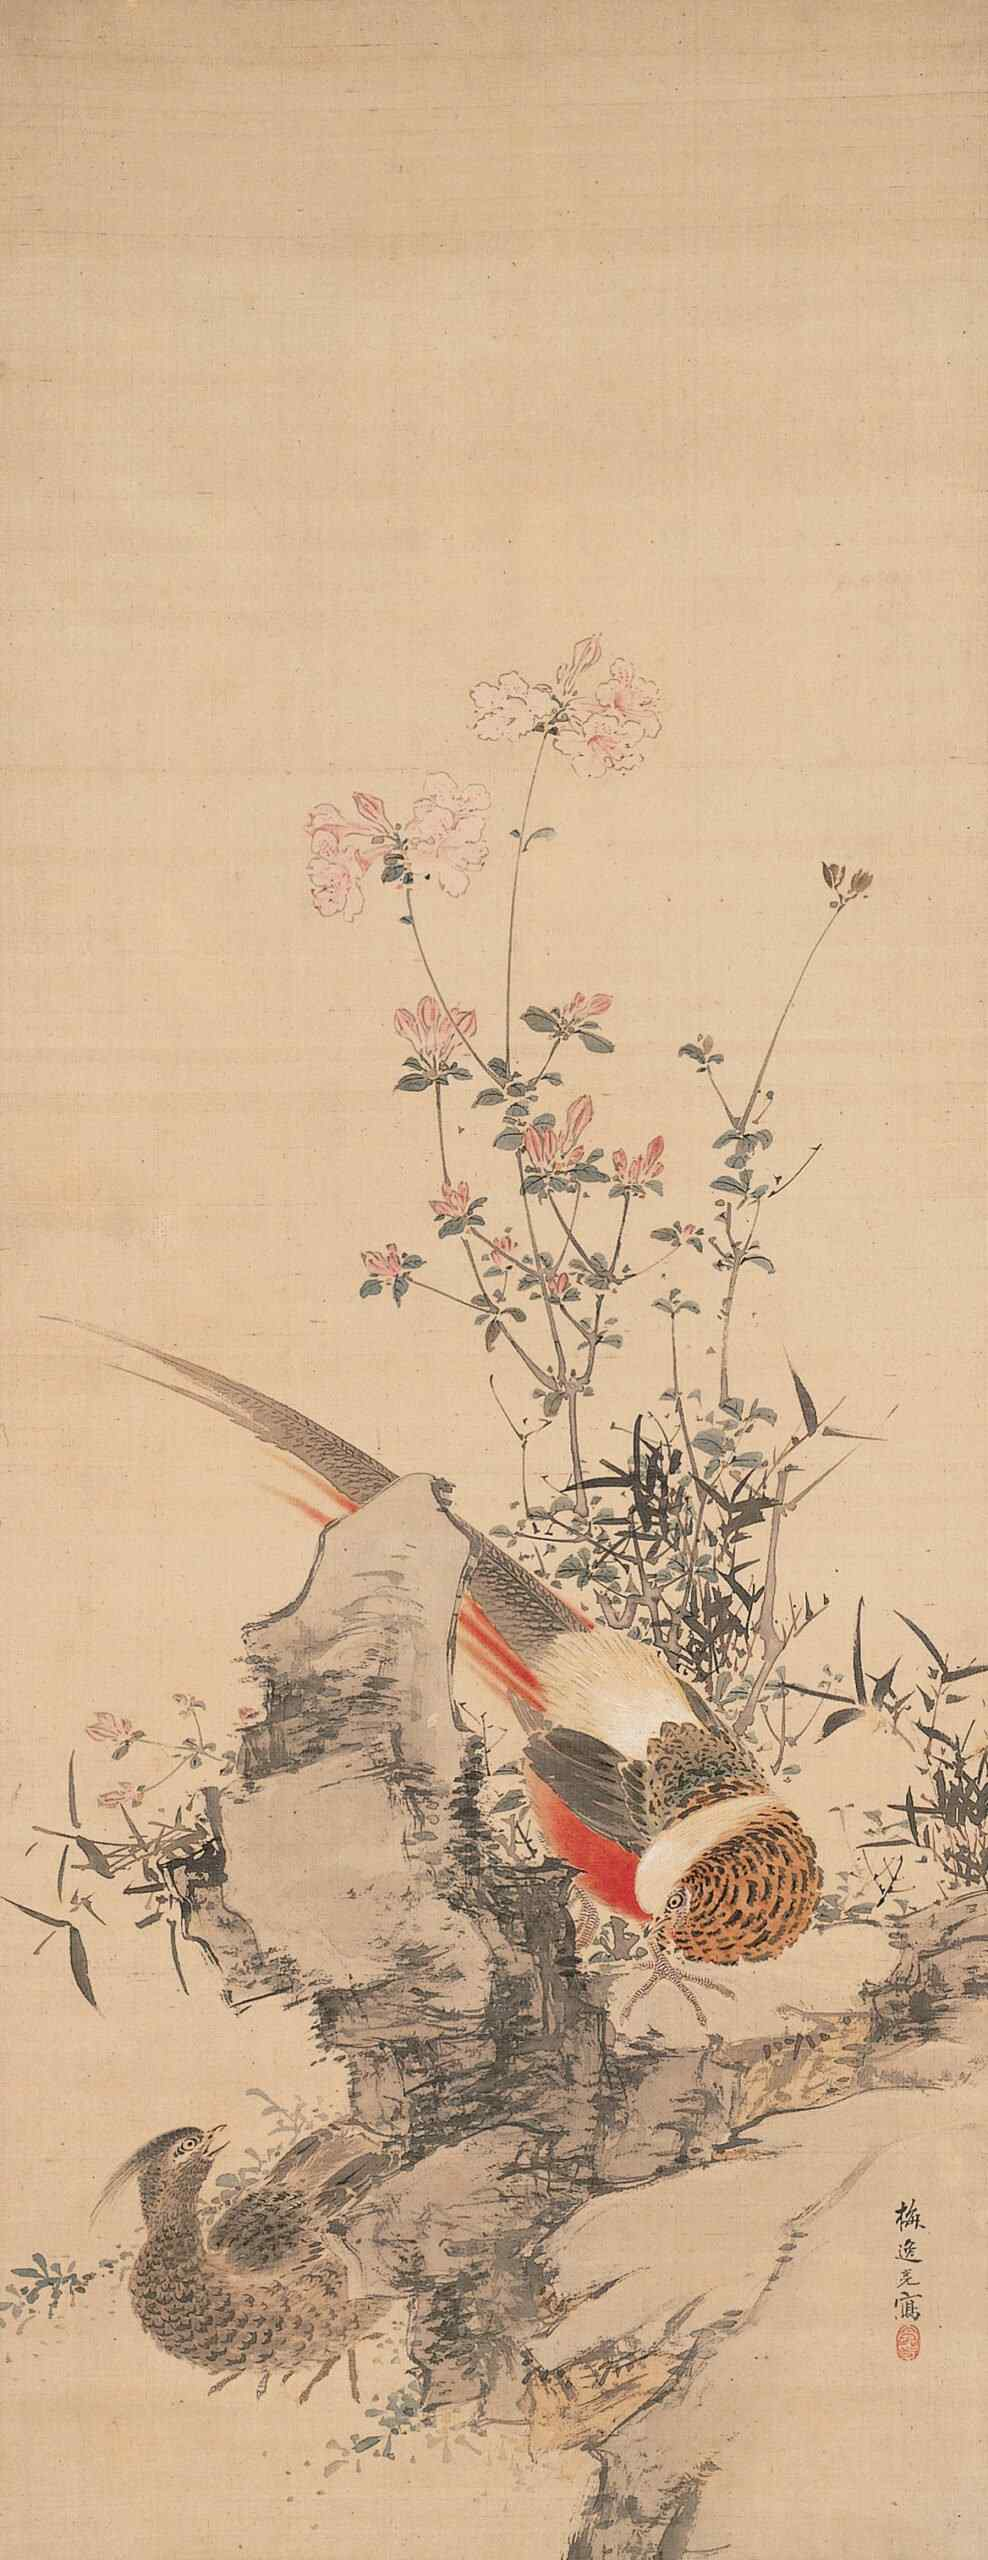
\includegraphics{../img/image10.jpg}

\begin{verseblock}

\newpage

\begin{center}\textbf{46.}\end{center}

得 失 是 非 一 時 放 卻

Dé shī shì fēi yī shí fàng què

Ganar y perder, correcto e incorrecto\ldots,\\
suéltalos de una vez.

\end{verseblock}

\hfill\break

\hypertarget{comentario-45}{%
\subsection{Comentario}\label{comentario-45}}

Cuando observamos la ganancia y pérdida, descubrimos que no son más que
interpretaciones que proyectamos sobre los hechos. En el giro incesante
de la existencia, lo que hoy nos parece una ganancia puede revelarse
mañana como una pérdida, y lo que hoy lamentamos podría abrir la puerta
a una oportunidad inesperada. Aferrarse a estas categorías nos encadena
al sufrimiento, porque nos resistimos a la verdadera naturaleza de la
vida: su constante transformación.

En la tradición budista, una de las tres marcas de la existencia es la
impermanencia. Todo lo que surge, cambia. Todo lo que cambia,
desaparece. Esta comprensión debe transformarse una una experiencia
vivida que encarne la naturaleza transitoria de todas las cosas.

Del mismo modo, las nociones de lo correcto y lo falso se desdibujan
cuando miramos con los ojos del despertar. Lo que una mente condicionada
considera correcto, otra puede juzgar erróneo, y viceversa. Contextos
culturales, marcos históricos, vivencias personales\ldots{} todo moldea
nuestras percepciones. Así, lo que creemos firmemente puede derrumbarse
ante una comprensión más amplia, más libre, más compasiva.

La práctica del Zen nos enseña a ir más allá de estas dualidades. A
través de la meditación, aprendemos a mirar sin filtros, a habitar el
instante presente sin aferrarnos a etiquetas, juicios ni narraciones. En
ese silencio claro, la realidad se muestra tal como es: sin división,
sin opuestos, sin conflictos.

Al contemplar la impermanencia con una mente abierta, dejamos de
perseguir la ganancia y de temer la pérdida. Ya no necesitamos
aferrarnos a lo correcto ni rechazar lo falso. Simplemente estamos. Y en
ese estar, libres de construcciones mentales, podemos encontrar la paz
profunda de quien ha dejado de luchar contra el río de la vida y ha
aprendido a fluir con él.

\hfill\break

\hypertarget{02}{}
\begin{verseblock}

\newpage

\begin{center}\textbf{47.}\end{center}

眼 若 不 睡 諸 夢 自 除

Yăn ruò bù shuì zhū mèng zì chú

Si los ojos no duermen,\\
todos los sueños desaparecen por sí mismos.

\end{verseblock}

\hfill\break

\hypertarget{comentario-46}{%
\subsection{Comentario}\label{comentario-46}}

El despertar es la enseñanza central y la experiencia más transformadora
en el budismo. De hecho, \emph{Buda} no es un nombre propio, sino un
epíteto que significa ``el despierto'': aquel que ha trascendido la
ignorancia y el sufrimiento para morar en una sabiduría serena y
compasiva. Este estado no está reservado a unos pocos; es una
posibilidad real al alcance de todos y todas. En ese camino, la atención
es la llave.

Cuando ``los ojos no duermen'' ---es decir, cuando cultivamos una
presencia lúcida, especialmente a través de la atención al cuerpo y a la
respiración--- comenzamos a habitar la experiencia con ecuanimidad. Sin
necesidad de luchar, reprimir o controlar, los contenidos mentales
---sueños, ilusiones y proyecciones--- comienzan a disolverse por sí
solos. La realidad se va revelando tal como es, sin adornos ni filtros.

En el Zen, utilizamos con frecuencia la metáfora del espejo para
clarificar esta enseñanza. Un espejo limpio refleja con nitidez lo que
tiene delante. Pero si está cubierto de polvo, la imagen se distorsiona
y confundimos lo que vemos. Del mismo modo, una mente clara y atenta
refleja fielmente la realidad. En cambio, una mente ofuscada por
pensamientos, juicios y emociones desbordadas genera confusión,
sufrimiento y separación.

Esta imagen está bellamente recogida en el conocido poema del
\href{https://www.daizansoriano.com/ta-chien-hui-neng/}{caso 34} del
\emph{Denkoroku}.

\begin{quote}
El cuerpo es el árbol de la iluminación,\\
la mente es un espejo resplandeciente.\\
Trata de mantenerlo siempre limpio\\
y no permitas que el polvo se acumule sobre él.
\end{quote}

Esta es una enseñanza parcial. La realización última va más allá incluso
de la limpieza del espejo. Así lo expresó el sexto patriarca Huineng en
su célebre respuesta:

\begin{quote}
La iluminación no es esencialmente un árbol,\\
ni hay tampoco espejo que resplandezca.\\
Desde el principio, no existe una sola cosa:\\
¿dónde podría, entonces, acumularse el polvo?
\end{quote}

Estas palabras no niegan la práctica, sino que apuntan más allá de toda
forma, más allá incluso de la idea de un ``yo'' que deba despertar.
Cuando la mirada está verdaderamente despierta, no hay nada que alcanzar
ni nada de lo que deshacerse. Solo queda esta presencia viva, clara y
libre, donde todos los sueños se disuelven como la niebla al amanecer.

\hfill\break

\hypertarget{03}{}
\begin{verseblock}

\newpage

\begin{center}\textbf{48.}\end{center}

心 若 不 異 萬 法 一 如

Xīn ruò bù yì wàn fă yī rú

Cuando la mente no discrimina,\\
los diez mil dharmas son uno.

\end{verseblock}

\hfill\break

\hypertarget{comentario-47}{%
\subsection{Comentario}\label{comentario-47}}

Cuando cesamos de dividir, clasificar y oponer, se revela la unidad
fundamental de la existencia. Los ``diez mil dharmas'' ---es decir,
todos los fenómenos del universo--- no son cosas separadas, sino
expresiones interdependientes de una misma realidad. Comprender esto no
es una mera idea filosófica, sino una realización profunda, como una
llave que abre la puerta al estado de no-dualidad. Es la experiencia de
una mente que ha trascendido la compulsión de separar entre ``esto'' y
``aquello'', entre ``yo'' y ``el mundo'', entre ``correcto'' y
``equivocado''. Una mente unificada, sin fisuras, que no toma partido ni
por ni contra.

Se trata de cultivar una mente sin preferencias, sin etiquetas. Una
mente abierta y receptiva, capaz de acoger la realidad tal como es, sin
separarla en bueno y malo, correcto o incorrecto, sagrado o profano.
Practicar esta no discriminación no significa volverse indiferente, sino
despertar a una sabiduría compasiva que reconoce la interconexión de
todos los seres. Al soltar las categorías rígidas, el corazón se
ensancha y la vida se unifica.

Y entonces, como una consecuencia natural ---no como una conquista---,
los ``diez mil dharmas son uno''. Las cosas no desaparecen ni se funden
en un vacío homogéneo. No es que todo se vuelva igual, sino que se
reconoce lo uno en lo múltiple. Cada cosa es tal como es ---única,
irrepetible--- pero no está separada de nada. Las olas distintas del mar
no dejan de ser olas, pero son solo el mar. Las diez mil cosas ---todos
los fenómenos del mundo--- siguen siendo múltiples, pero ya no están
desgajadas del corazón de la realidad.

Es una visión en la que la diversidad no es contradicción, sino
expresión de la unidad. Cuando dejamos de proyectar nuestras
preferencias, cuando cesa la mente que toma partido, lo que queda es una
gran inclusividad: todo tiene su lugar, todo está interconectado, todo
es, simplemente, así como es.

Y esto no es un ideal lejano, sino una forma de ver que se cultiva
momento a momento en la práctica de zazen: sentarse sin tomar partido,
sin dividir, sin construir un yo frente a las cosas. Entonces la mente
descansa. Y en ese descanso, el mundo entero se vuelve íntimo.

\hfill\break

\hypertarget{04}{}
\begin{verseblock}

\newpage

\begin{center}\textbf{49.}\end{center}

一 如 體 玄 兀 爾 忘 縁

Yī rú tĭ xuán wù ěr wàng yuán

En la unidad, se realiza la esencia profunda,\\
sin esfuerzo, los apegos se disuelven.

\end{verseblock}

\hfill\break

\hypertarget{comentario-48}{%
\subsection{Comentario}\label{comentario-48}}

Todo en este universo está interconectado. Nada existe por sí solo. Cada
ser, cada cosa, cada instante, forma parte de una red viva de
interdependencia. Esta es una enseñanza fundamental del budismo: no hay
separación, no hay un ``yo'' aislado, no hay un ``esto'' frente a
``aquello''.

Cuando nos sentamos en zazen y soltamos nuestras ideas, juicios
condicionados y expectativas, comienza a revelarse una unidad silenciosa
que no necesita ser entendida, solo reconocida. No es una comprensión
intelectual, sino un despertar natural, sin esfuerzo.

Cuando la mente descansa en la unidad, las nociones de causa y efecto,
de tiempo y progreso, se diluyen. Ya no hay un punto de partida ni una
meta. Solo este momento, completo en sí mismo. Al cesar la agitación,
los apegos se disuelven por sí solos. No porque los forcemos a
desaparecer, sino porque ya no tienen de dónde agarrarse. En el silencio
de la práctica, lo que parecía sólido se vuelve fluido. Lo que parecía
separado, se revela como uno.

Esta es la esencia de la vía: no hacer nada especial, no perseguir nada.
Simplemente sentarse, con el cuerpo en quietud y el corazón abierto.
Permitir que la vida sea como es. En esta forma de estar, encontramos
una sabiduría que no depende del pensamiento y una compasión que no
necesita esfuerzo. Vivir desde esta unidad es vivir con autenticidad,
sin necesidad de adornos, sin miedo a la imperfección.

Zazen no es una técnica ni un medio para alcanzar algo. Es el retorno
natural a lo que siempre ha estado aquí. Cuando la mente deja de
dividir, el mundo entero se vuelve íntimo.

\hfill\break

\hypertarget{05}{}
\begin{verseblock}

\newpage

\begin{center}\textbf{50.}\end{center}

萬 法 齊 觀 歸 復 自 然

Wàn fă qí guān guī fù zì rán

Cuando todos los fenómenos son contemplados con ecuanimidad,\\
retornan a su naturaleza original.

\end{verseblock}

\hfill\break

\hypertarget{comentario-49}{%
\subsection{Comentario}\label{comentario-49}}

En el bullicio y el caos de la vida cotidiana, nos vemos inmersos en un
mar de emociones y experiencias que nos arrastran en diferentes
direcciones. En medio de este torbellino surgen el conflicto y el
sufrimiento. Anhelamos la calma y la serenidad. Pero, ¿cómo encontrar
tranquilidad en un mundo tan turbulento?

La tradición Zen nos ofrece un camino diferente a este caos a través del
cultivo sistemático de la ecuanimidad y la aceptación. Contemplando la
realidad con equilibrio y una presencia serena. La ecuanimidad nos da la
capacidad de observar el flujo de la vida sin ser arrastrados por sus
oleajes. Nos permite mantenernos en calma, incluso en medio de las
tormentas más intensas. Como quien aprende a surfear las olas sin
hundirse en ellas.

La práctica de zazen cultiva en nosotros esta mirada ecuánime. Nos
enseña a permitir que las cosas sean tal como son, sin juicio ni
resistencia. En este estado de aceptación, cada experiencia retorna a su
esencia: nada sobra, nada falta. Lo que parecía un obstáculo se revela
como enseñanza. En lugar de luchar contra la corriente de la vida, nos
abrimos a su ritmo natural, encontrando paz y armonía instante a
instante.

La aceptación es confianza. Es aprender a abrazar la realidad tal como
es, sin intentar forzarla ni controlarla. Y en ese gesto de rendición
---que no es resignación--- encontramos una profunda libertad: la
libertad de soltar nuestras exigencias, nuestras expectativas, nuestros
deseos no satisfechos.

Cuando aceptamos plenamente lo que es, brota una paz silenciosa. Ya no
luchamos. Dejamos de resistirnos, y el sufrimiento pierde fuerza.
Entonces, podemos sumergirnos en el fluir de la vida con el corazón
abierto, habitando cada momento con serenidad, incluso en medio de la
impermanencia.

\hfill\break

\hfill\break

\hypertarget{01}{}
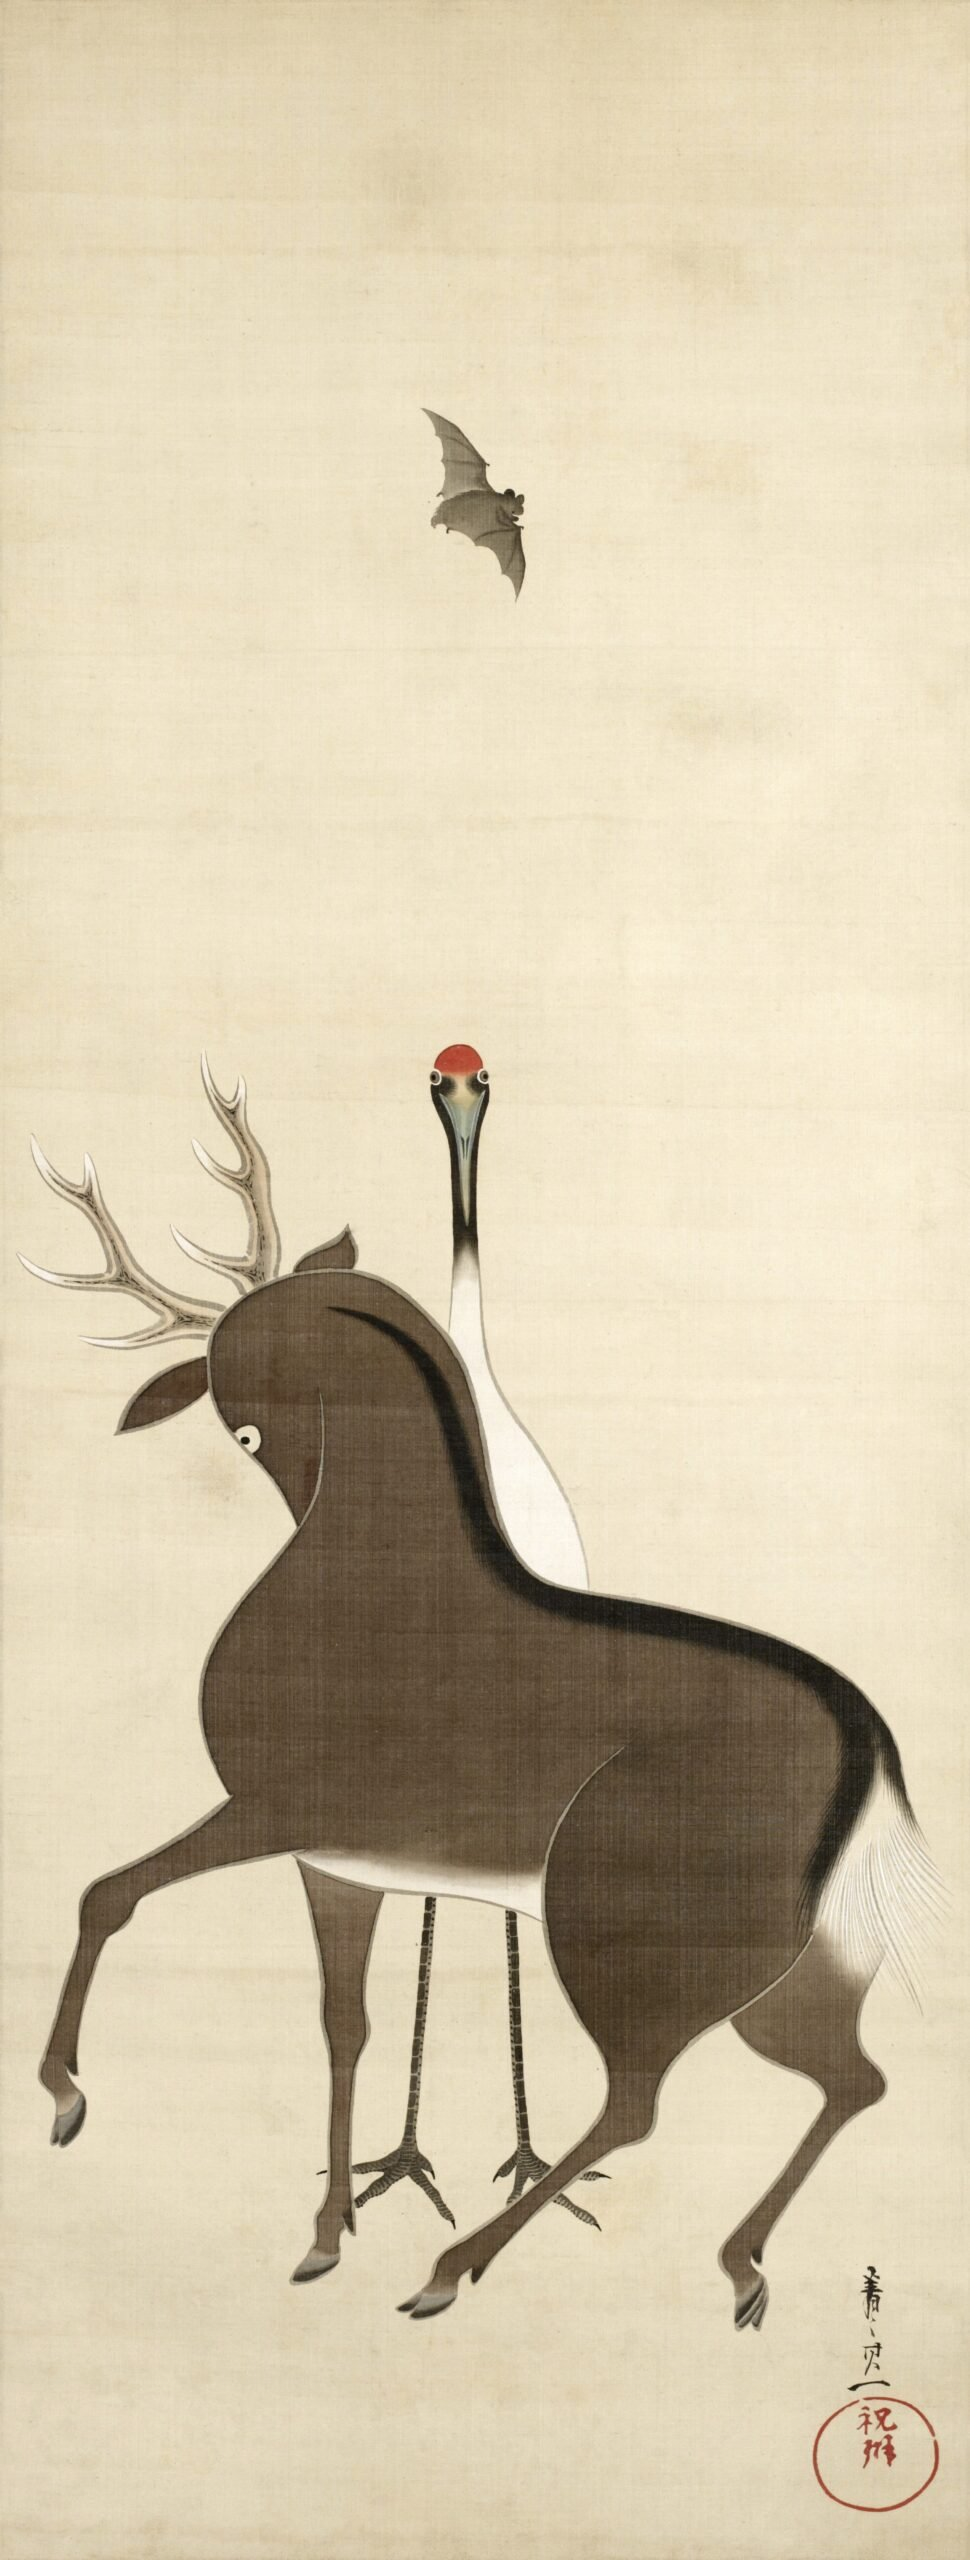
\includegraphics{../img/image11.jpg}

\begin{verseblock}

\newpage

\begin{center}\textbf{51.}\end{center}

泯 其 所 以 不 可 方 比

Mĭn qí suŏ yĭ bù kě fāng bĭ

Cuando desaparece cualquier estructura conceptual,\\
la verdad última no puede ser atrapada con palabras.

\end{verseblock}

\hfill\break

\hypertarget{comentario-50}{%
\subsection{Comentario}\label{comentario-50}}

En la tradición zen solemos usar la metáfora del agua clara. Imagina un
recipiente lleno de agua fangosa, donde el cieno ensucia su
transparencia. Al agitarlo, no podemos ver el fondo; todo se confunde.
Pero si lo dejamos reposar, las impurezas se asientan y la claridad
aparece por sí sola. ¿Qué ocurre cuando el agua está completamente
limpia? Ya no hay medida ni comparación. No podemos decir que hoy está
más clara que ayer, porque no queda resto de turbiedad con el que
establecer diferencia. Solo queda la claridad misma, perfecta en su
transparencia, sin necesidad de calificativos.

Así es también la mente cuando deja de aferrarse a conceptos, juicios y
expectativas. Cuando nos sentamos en zazen y permitimos que los
pensamientos se asienten sin alimentarlos, comenzamos a experimentar esa
apertura natural. No es algo que se alcance por esfuerzo, sino que
emerge cuando dejamos de intervenir.

La verdad última no puede expresarse con palabras porque está más allá
de todo marco conceptual. Es como el agua cristalina: puedes verla,
puedes sentir su frescor, pero en cuanto intentas encerrarla en una
forma fija, se te escurre entre los dedos.

En la práctica del zen, aprendemos a confiar en esta claridad. No
buscamos adornos ni certezas. Solo estar plenamente presentes, libres
del juego interminable de la comparación. Y en esa presencia,
descubrimos una forma más auténtica de vivir, en armonía con lo que es.

Ser como el agua clara no significa perfección en términos comunes.
Significa permitir que lo que somos se exprese sin obstrucción. Cada
paso en el camino es una oportunidad para afinar esa transparencia, para
abrazar la autenticidad y la compasión, tanto hacia las demás personas
como hacia uno/a mismo/a.

\hfill\break

\hypertarget{02}{}
\begin{verseblock}

\newpage

\begin{center}\textbf{52.}\end{center}

止 動 無 動 動 止 無 止

Zhĭ dòng wú dòng Dòng zhĭ wú zhĭ

Cuando la quietud detiene el movimiento, no hay movimiento.\\
Cuando el movimiento detiene la quietud, no hay quietud.

\end{verseblock}

\hfill\break

\hypertarget{comentario-51}{%
\subsection{Comentario}\label{comentario-51}}

Movimiento y quietud parecen dos realidades opuestas, pero no pueden
existir la una sin la otra. Son expresiones de una misma verdad,
profundamente entrelazadas. En zazen, la meditación sentada, no buscamos
simplemente inmovilidad externa. La quietud que cultivamos es más sutil:
una serenidad profunda que surge cuando dejamos de seguir los
pensamientos, cuando la mente deja de agitar la superficie del instante.
Esta quietud no es rigidez, ni pasividad; es apertura, presencia, un
espacio interior desde el cual todo puede emerger.

Con el tiempo, esta práctica va aquietando las olas del pensamiento y
del deseo. Y desde ese fondo claro, desde ese océano silencioso,
empezamos a ver con mayor nitidez lo que somos y lo que es. La mente,
libre de turbulencias, se vuelve como un espejo limpio: refleja el mundo
tal como es, sin distorsión.

Pero esta quietud no está vacía. Es como el fondo del océano:
aparentemente inmóvil, pero lleno de vida latente, de energía contenida.
Desde esta quietud, el bodhisattva ---la persona que despierta para el
bien de todos los seres--- actúa. No desde la agitación del ego, sino
desde la calma que conoce la interconexión de todas las cosas. En esa
quietud madura la compasión, brota la sabiduría.

Imagina que viajas en tren y observas el paisaje que pasa veloz tras la
ventanilla. ¿Quién se mueve, tú o el mundo? La experiencia del
movimiento o de la quietud no está en las cosas mismas, sino en la forma
en que nos relacionamos con ellas. Es la mente la que define el punto de
referencia.

La práctica de zazen nos permite soltar ese punto fijo. Nos enseña a
habitar el instante sin aferrarnos, a descubrir que en el corazón de la
quietud también hay movimiento, y que en el movimiento más dinámico
puede habitar una calma profunda.

Desde esta raíz serena, nuestros actos pueden nacer con claridad.
Nuestra vida entera se convierte en una expresión del equilibrio entre
el reposo y la acción, entre el silencio y la palabra, entre el estar y
el hacer. Y así, paso a paso, cultivamos una presencia compasiva, una
sabiduría encarnada en la vida cotidiana.

\hfill\break

\hypertarget{03}{}
\begin{verseblock}

\newpage

\begin{center}\textbf{53.}\end{center}

兩 既 不 成 一 何 有 爾

Liăng jì bù chéng yī hé yŏu ěr

Si la dualidad no existe,\\
¿Cómo puede haber unidad?

\end{verseblock}

\hfill\break

\hypertarget{comentario-52}{%
\subsection{Comentario}\label{comentario-52}}

Si no hay dos, ¿qué sentido tiene hablar de uno? La idea de unidad solo
surge cuando hay algo de lo que distinguirse. En nuestro modo habitual
de percibir, nos movemos entre pares de opuestos: luz y sombra, gozo y
dolor, sonido y silencio. Pero ninguno de estos polos tiene existencia
propia sin el otro. No podemos comprender la claridad sin haber conocido
la oscuridad, ni saborear la alegría sin haber tocado antes la tristeza.
La vida y la muerte, la expansión y el repliegue, el día y la noche, lo
femenino y lo masculino, lo que comienza y lo que concluye. Todo se
entreteje en una red de interdependencia que no deja lugar para
entidades separadas o realidades absolutas.

Desde la visión del Budadharma, no se trata de negar la dualidad, ni de
aferrarse a la unidad como un ideal supremo. Se trata de ver cómo ambos
conceptos surgen de la misma mente que discrimina, nombra y compara.
Cuando soltamos esa mente, cuando dejamos de lado la necesidad de
definir, clasificar y oponer, lo que queda no es una verdad única y
cerrada, sino una realidad viva donde cada cosa se manifiesta en íntima
conexión con todo lo demás.

La práctica de zazen nos permite habitar ese espacio donde los opuestos
no luchan entre sí, sino que se disuelven en una presencia silenciosa y
total. Al sentarnos sin buscar nada, sin rechazar nada, comenzamos a
vislumbrar una dimensión que no pertenece ni a la dualidad ni a la
unidad, sino a lo que simplemente es.

En esa claridad, vemos que la mente que crea la separación es la misma
que ansía la unificación. Y al ver eso, dejamos de seguir el juego. Solo
entonces podemos habitar el instante tal como es, sin necesidad de
elegir entre esto o aquello, entre ser uno o ser dos.

Desde ese lugar, vivimos con más ligereza. Nos abrimos a la
impermanencia, a la contradicción, al misterio. Y en lugar de temer la
complejidad de la vida, la honramos. Porque entendemos que no hay un
lado correcto al que aferrarse, sino un flujo continuo que nos invita a
soltar, mirar y simplemente estar.

\hfill\break

\hypertarget{04}{}
\begin{verseblock}

\newpage

\begin{center}\textbf{54.}\end{center}

究 竟 窮 極 不 存 軌 則

Jiū jìng qióng jí bù cún guĭ zé

La realización última y absoluta,\\
no sigue ninguna regla establecida.

\end{verseblock}

\hfill\break

\hypertarget{comentario-53}{%
\subsection{Comentario}\label{comentario-53}}

La sabiduría no consiste en acumular teorías ni en aferrarse a
conceptos. Es un proceso de autodescubrimiento, una transformación
profunda que va más allá de las categorías del pensamiento. A diferencia
de la tradición occidental, que a menudo presenta al santo como ideal
moral a seguir, el budismo pone en valor la figura del sabio o de la
persona despierta: alguien que no imita, sino que busca, que duda, que
se deja interpelar por lo real.

Pero este camino de búsqueda también tiene sus trampas. Una de las más
sutiles es la obsesión por alcanzar una comprensión definitiva, un punto
final donde todo quede resuelto. Esa obsesión nos aleja del corazón
mismo del budismo: la vacuidad.

La vacuidad nos muestra que todos los fenómenos ---incluidas nuestras
ideas, creencias y certezas--- carecen de esencia propia. Todo es
transitorio, interdependiente, cambiante. Por eso, cualquier intento de
fijar una verdad última como una ley o doctrina inmutable está destinado
al fracaso. Toda regla que impongamos a la realidad, por noble o
refinada que sea, es una construcción mental más, y por tanto, vacía.

Frente a este abismo de impermanencia, solo cabe la honestidad.
Comprender la vacuidad no significa resignarse al sinsentido, sino abrir
el corazón a una sabiduría más profunda: la de no saber, la de estar
presente sin aferrarse. La verdadera realización no se alcanza por
acumulación de respuestas, sino por rendición del ego, por soltar el
impulso de controlar y permitir que la experiencia hable por sí misma.

En una historia que he escuchado muchas veces a mi maestro, se ilustra
esta paradoja con la sencillez de una escena cotidiana:

Un erudito budista, especialista en el Sutra del Diamante, viajaba hacia
un templo donde un maestro zen iba a dar una enseñanza sobre dicho
texto. Caminaba con aire altivo, cargado de volúmenes y conocimientos.
En su camino, se encontró con una anciana que vendía pasteles de arroz.
Al ver los libros, la anciana le preguntó qué eran. El erudito respondió
con suficiencia: "Son copias del Sutra del Diamante, que estudio y
enseño".

La anciana sonrió y le ofreció un trato: ---Si puedes responder a una
pregunta sobre ese sutra, te regalaré tantos pasteles como desees. Si no
puedes, te irás con el estómago vacío.

Intrigado, el erudito aceptó.

La anciana dijo: ---En el sutra se afirma: La mente del pasado es
vacuidad. La mente del presente es vacuidad. La mente del futuro es
vacuidad. Dime entonces, ¿con qué mente vas a comerte mis pasteles de
arroz?

El erudito enmudeció. De pronto, toda su erudición quedó expuesta como
un castillo de arena. Incapaz de responder, comprendió que la anciana
---sin títulos ni reconocimiento--- encarnaba una comprensión que él aún
no había alcanzado. Avergonzado, dio media vuelta y se marchó.

Esta historia, sencilla pero afilada como una espada, nos recuerda que
la verdadera sabiduría no se encuentra en las palabras, sino en la
experiencia directa, libre de orgullo y de intención. Como decía Jianzhi
Sengcan, la realización última no obedece a ninguna fórmula. No puede
ser atrapada ni organizada, solo vivida.

En el fondo de la simplicidad habita una claridad que trasciende el
tiempo, los dogmas y las estructuras. Es ahí, en ese espacio desnudo de
la mente, donde brota una sabiduría real: la que nace de la humildad, la
honestidad y la entrega total al instante presente.

\hfill\break

\hypertarget{05}{}
\begin{verseblock}

\newpage

\begin{center}\textbf{55.}\end{center}

契 心 平 等 所 作 倶 息

Qì xīn píng děng, suŏ zuò jù xī

Cuando la mente alcanza la ecuanimidad,\\
todo movimiento se aquieta.

\end{verseblock}

\hfill\break

\hypertarget{comentario-54}{%
\subsection{Comentario}\label{comentario-54}}

Ecuanimidad no es indiferencia ni frialdad. Es el equilibrio natural de
la mente cuando deja de dejarse arrastrar por las olas del agrado y el
rechazo. Cuando en zazen soltamos todo juicio y nos limitamos a estar
plenamente presentes, sin aferrarnos a nada y sin empujar nada, se
revela una cualidad silenciosa y estable: la ecuanimidad, cultivada
sistemáticamente a través de la concentración en el cuerpo y la
respiración, fundiéndonos en esta experiencia.

En este estado, no buscamos alcanzar nada especial. Simplemente estamos.
Y en ese estar completo, sin fisuras, el movimiento compulsivo de la
mente empieza a detenerse. No porque lo forcemos, sino porque ya no
tiene de qué alimentarse. La mente se aquieta como un estanque al que ya
no se le lanzan piedras. El deseo de que las cosas sean distintas
desaparece. La resistencia también. Todo se iguala en la claridad del
momento presente.

Este aquietamiento no implica pasividad interior. Por el contrario, es
una forma de estar radicalmente vivo/a, abierto/a a todo lo que sucede.
Pero ese vivir ya no está teñido por la agitación del ``yo'', por la
constante oscilación entre ``quiero esto'' y ``no quiero aquello''.
Desde la ecuanimidad, cada fenómeno surge y desaparece como una nube en
el cielo, sin dejar huella.

En esa quietud que no rechaza, el ego deja de moverse. Se disuelven las
prisas, la comparación, el afán de control. Y lo que permanece es una
mente que refleja la realidad tal como es, sin interferencia. Una mente
que, como el agua clara, no añade nada ni quita nada.

Desde ahí, nuestras acciones nacen con naturalidad, sin tensión. No
reaccionamos: respondemos. No actuamos por impulso, sino desde la
sintonía con lo real. Esta es la actividad del bodhisattva: actuar sin
ser arrastrado por los vaivenes de la mente condicionada, ofreciendo
calma y claridad a un mundo lleno de ruido.

Cuando la mente alcanza la ecuanimidad, no hay nada que empujar, nada
que retener. Todo movimiento se aquieta. Y en esa quietud, se revela una
paz profunda que no depende de las circunstancias, ni del resultado, ni
del esfuerzo. Una paz que ya estaba ahí, esperando ser reconocida.

\hfill\break

\hfill\break

\hypertarget{01}{}
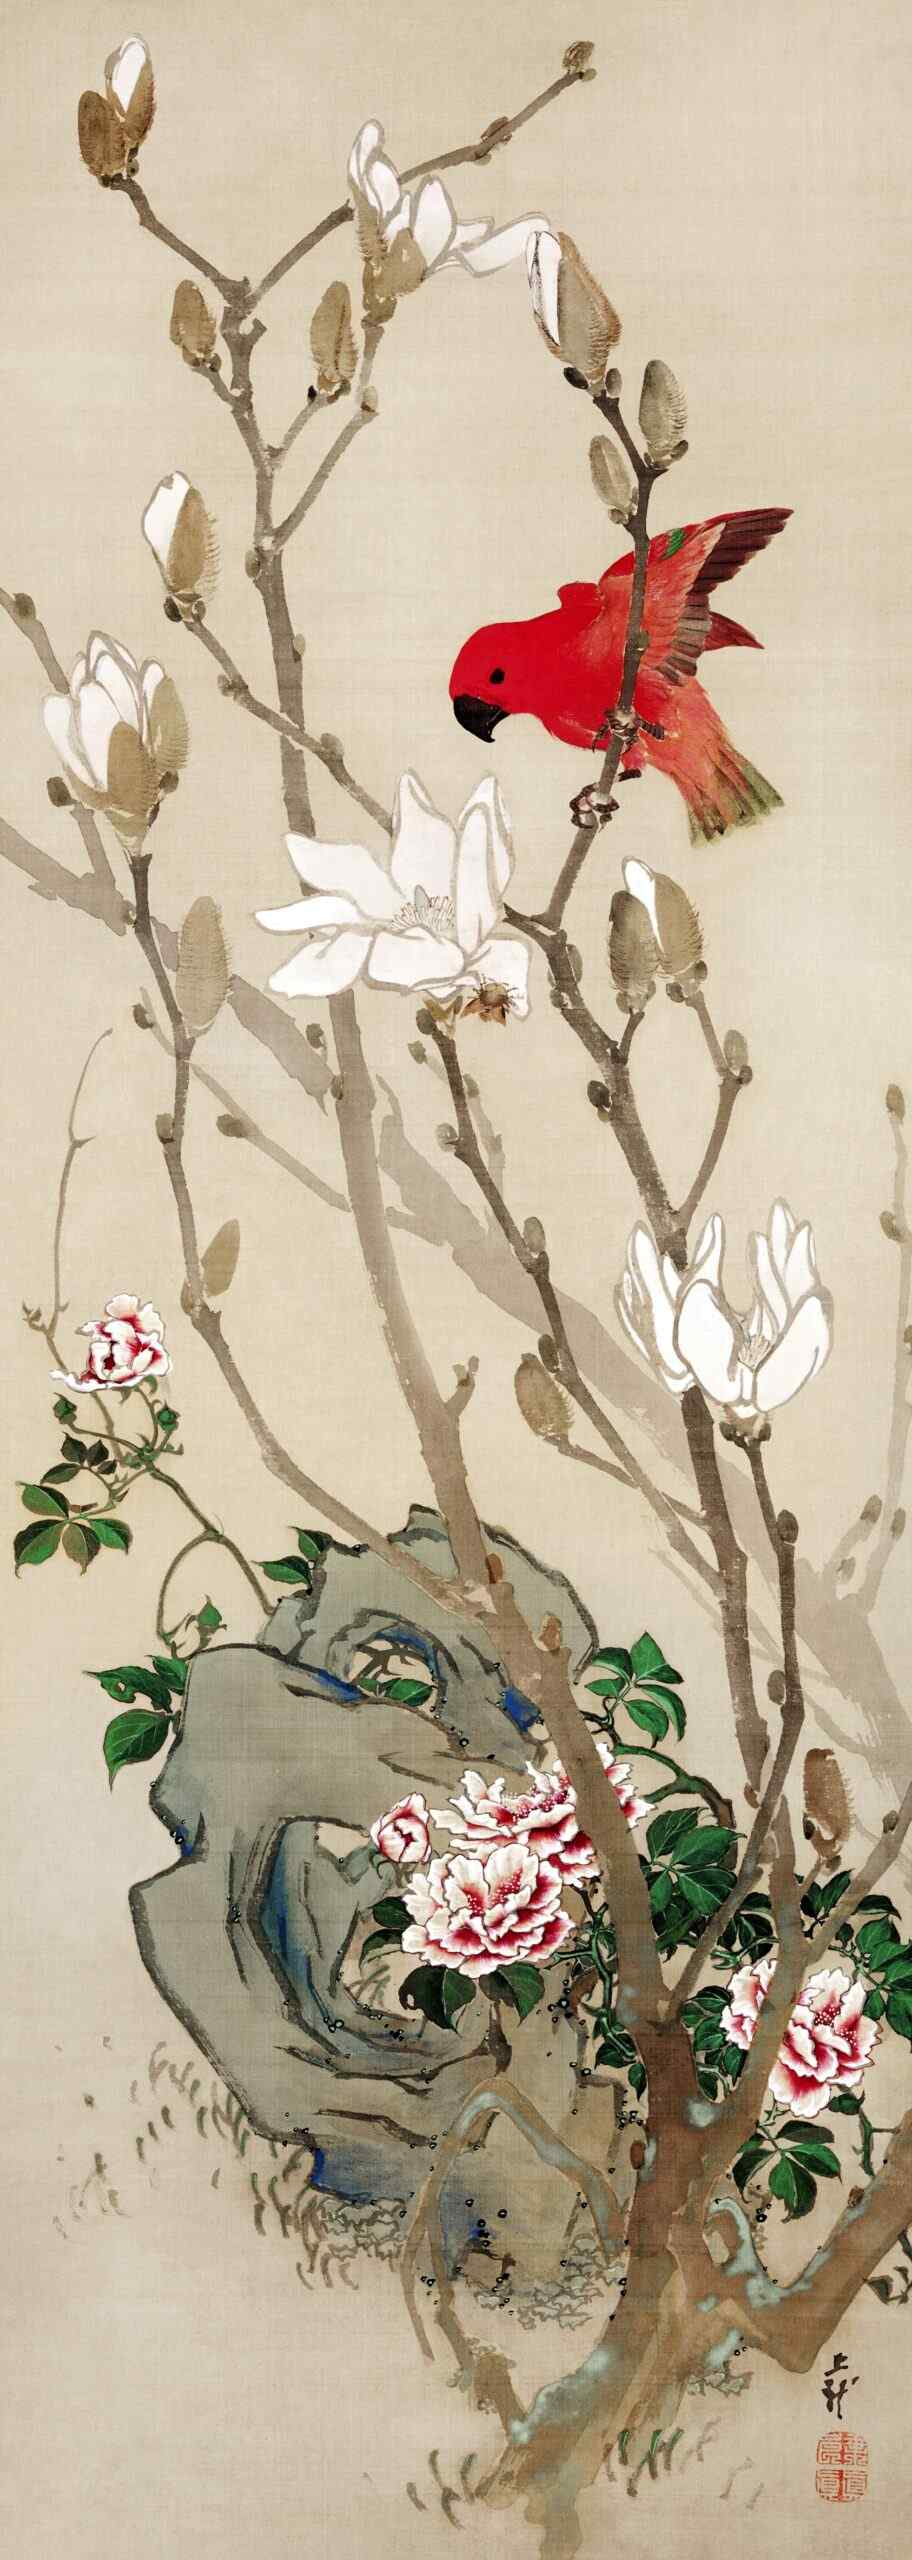
\includegraphics{../img/image12.jpg}

\begin{verseblock}

\newpage

\begin{center}\textbf{56.}\end{center}

狐 疑 盡 淨 正 信 調 直

Hú yí jìn jìng zhèng xìn diào zhí

Cuando las dudas se disipan por completo,\\
la confianza se vuelve serena y armoniosa.

\end{verseblock}

\hfill\break

\hypertarget{comentario-55}{%
\subsection{Comentario}\label{comentario-55}}

Uno de los cinco obstáculos clásicos en el Budadharma es la duda. En
nuestro camino es importante tomar conciencia de ella para transformarla
en una confianza sincera y armoniosa. Las dudas son como sombras que, en
silencio, obstaculizan el camino hacia la comprensión profunda y la
realización. En el zen decimos: ``pequeña duda, pequeña iluminación;
gran duda, gran iluminación''. Porque, como todos los obstáculos, la
duda puede convertirse en una oportunidad valiosa de introspección y
claridad.

No hay que temer a la duda, sino acogerla con honestidad y lucidez.
Existen muchas formas de dudar: podemos dudar de nuestra propia
capacidad, de la enseñanza, del maestro, del Buda o incluso del camino
en sí. A veces dudamos porque el ego se resiste a soltar el control;
otras veces, porque hemos sido heridos y desconfiamos. Y otras, porque
simplemente aún no hemos visto con claridad.

La duda aparece cuando la mente se topa con sus propios límites, cuando
las ideas fijas comienzan a resquebrajarse. Y justo ahí, si no huimos,
puede abrirse una puerta. A menudo, las dudas más persistentes no son
intelectuales, sino existenciales. No dudamos solo de conceptos, sino de
nuestro lugar en el mundo, de nuestra capacidad de amar, de soltar, de
entregarnos. Por eso, la práctica no consiste en suprimirlas, sino en
acompañarlas con presencia, sin necesidad de respuestas inmediatas.

A través de zazen, el estudio del Dharma y el encuentro con las
enseñanzas de los maestros, aprendemos a atravesar la niebla de la
confusión. No se trata de acumular respuestas, sino de descubrir la
verdad que habita en lo más profundo de nuestra consciencia. Con cada
respiración consciente y cada instante de plena atención, la mente se
aquieta y se vuelve transparente, revelando la naturaleza de la realidad
tal como es.

A medida que la niebla de la duda se disipa, la confianza surge de forma
natural, sin esfuerzo. No es una fe ciega ni una creencia impuesta, sino
una confianza que nace de la experiencia directa y de una comprensión
íntima y viva. Es la confianza en el proceso de la vida, en la
interdependencia de todas las cosas, en el camino que se revela paso a
paso bajo nuestros pies.

Esta confianza serena no nos promete certezas, pero nos sostiene incluso
cuando no las hay. Nos da raíces cuando todo se tambalea. Nos permite
quedarnos donde estamos, aunque lo que sintamos sea incertidumbre,
tristeza o no-saber. Cuando esta confianza nos acompaña, el corazón y la
mente se alinean armoniosamente. La lucha interna se desvanece, y en su
lugar brotan la paz y la claridad.

Esta armonía interior transforma nuestra forma de estar en el mundo: se
refleja en nuestras relaciones, en nuestras palabras y acciones, en cada
gesto de bondad y compasión. Así, la confianza cultivada en la práctica
nutre no solo nuestro bienestar, sino también el de todos los seres. La
duda se disuelve no porque desaparezca, sino porque deja de tener el
poder de separarnos de la vida.

\hfill\break

\hypertarget{02}{}
\begin{verseblock}

\newpage

\begin{center}\textbf{57.}\end{center}

一 切 不 留 無 可 記 憶

Yî qiè bù liú wú ke jì yì

Todo se disuelve sin dejar rastro,\\
no queda huella en la memoria.

\end{verseblock}

\hfill\break

\hypertarget{comentario-56}{%
\subsection{Comentario}\label{comentario-56}}

Todas las experiencias son impermanentes, están en constante cambio.
Nada permanece fijo. Nada se detiene. No hay nada que no fluya y
finalmente se disuelva sin dejar rastro.

Zazen nos entrena, de forma directa y sencilla, a permanecer sin
movernos ante lo que aparece y desaparece. Esta disposición natural
genera, con el tiempo, una ecuanimidad profunda: no una actitud pasiva,
sino una presencia viva, clara y libre.

Vivir desde la ecuanimidad no significa reprimir el dolor ni negar la
alegría, sino verlas tal como son: olas que vienen y van, sin dejar
rastro en el océano profundo. Esta sabiduría no nace de la teoría, sino
de la práctica perseverante. Con el tiempo, se convierte en una
fortaleza interior, en una fuente inagotable de compasión y
discernimiento.

Una de las historias más conmovedoras de nuestra tradición que ilustra
esta enseñanza es la del cuenco de mostaza:

Una mujer desesperada por la muerte de su hijo acudió al Buda,
suplicándole que lo devolviera a la vida. El Buda, con infinita
compasión, le pidió que trajera un puñado de mostaza de una casa donde
nunca hubiera muerto nadie. La mujer recorrió muchas casas, pero en
todas había habido pérdidas. Comprendió entonces, sin que nadie se lo
dijera, que la muerte forma parte de la vida. Y en esa aceptación
silenciosa, su corazón comenzó a sanar.

Generalmente damos por cierta nuestra memoria, pero esta es frágil,
maleable, incompleta. Está teñida por emociones, por el paso del tiempo,
por narrativas que inventamos sin darnos cuenta. Reconocer esta
fragilidad no es motivo de inquietud, sino una oportunidad para soltar
la rigidez de nuestras opiniones y abrirnos a una percepción más lúcida
y compasiva.

La memoria, aunque ilusoria en gran medida, cumple su función: nos da
una sensación de continuidad, de identidad. Pero en la práctica,
aprendemos a no tomarla por absoluta. Al fin y al cabo, despertar es
disolver nuestras fabricaciones mentales, dejar que todo se disuelva sin
aferrarnos. Y en ese vacío fértil, descubrimos nuestra naturaleza de
buda.

\hfill\break

\hypertarget{03}{}
\begin{verseblock}

\newpage

\begin{center}\textbf{58.}\end{center}

虚 明 自 照 不 勞 心 力

Xū míng zì zhào bù láo xīn lì

La vacuidad luminosa resplandece por sí misma,\\
sin hacer ningún esfuerzo mental.

\end{verseblock}

\hfill\break

\hypertarget{comentario-57}{%
\subsection{Comentario}\label{comentario-57}}

La verdadera comprensión y sabiduría no emergen de un esfuerzo mental
agotador ni de un análisis intelectual tenaz, sino de un estado de
receptividad tranquila y apertura, sin exclusiones. En el momento en que
dejamos ir las construcciones mentales automáticas del ego, esos
pensamientos que nunca cesan, es cuando el resplandor natural de nuestra
auténtica naturaleza se puede expresar con libertad. En el budismo zen,
hablamos de esto como la «Mente de Principiante», una mentalidad que nos
permite mirar el mundo con ojos frescos, renovados en cada instante, sin
el peso de nuestras preconcepciones ilusorias ni las construcciones
mentales automatizadas.

Para liberarnos de ese esfuerzo mental innecesario, debemos cultivar una
profunda confianza interna. Esta confianza nos conecta con nuestra
verdadera naturaleza original, permitiéndonos trascender el apego al yo
de manera natural, sin sobreesfuerzo. Tampoco se trata de una creencia
ciega, sino de una experiencia directa, un acto de confianza honesto.

Para desarrollar esta confianza, es necesario primero ser conscientes de
la estructura del «yo», y luego disolver esa identificación que hemos
hecho de manera ciega con nuestra personalidad. Este proceso puede ser
muchas veces doloroso, pues nos exige soltar una parte de nuestra
identidad y enfrentarnos a lo desconocido. La confianza serena, en este
caso, es el apoyo que necesitamos, pues nos da la seguridad de que todo
estará bien a pesar de las incertidumbres y vacíos que puedan surgir.

La confianza serena no se basa en confiar en algo concreto, sino en la
bondad intrínseca del universo. Es una disposición a dar el salto al
abismo, sin garantías de lo que sucederá, pero con la certeza de que
todo estará bien, sin importar las circunstancias. Esta confianza nos
permite vivir con valentía y autenticidad, sin luchar contra lo que es,
sin imponer esfuerzos innecesarios.

Cuando estamos anclados en esta confianza serena, vivimos nuestras vidas
con libertad y paz. Ya no nos paralizan el miedo ni la preocupación;
actuamos desde la seguridad de saber que estamos en el lugar adecuado,
haciendo lo que debemos hacer. La confianza serena nos permite
entregarnos completamente a la vida, soltar el control, y vivir en
armonía con la realidad tal como es.

\hfill\break

\hypertarget{04}{}
\begin{verseblock}

\newpage

\begin{center}\textbf{59.}\end{center}

非 思 量 處 識 情 難 測

Fēi sī liang chŭ shí qíng nán cè

Más allá del pensamiento,\\
la mente y las emociones son insondables.

\end{verseblock}

\hfill\break

\hypertarget{comentario-58}{%
\subsection{Comentario}\label{comentario-58}}

En la Vía del Zen, las paradojas aparentes nos guían a ir más allá de
nuestra comprensión habitual de la realidad. El pensamiento racional,
aunque esencial para nuestra vida cotidiana, tiene su valor limitado.
Nos ha permitido entender el mundo, desarrollar tecnologías y formar
sociedades complejas. Sin embargo, también se encuentra atrapado en
patrones rígidos, condicionado por nuestras experiencias, prejuicios y
deseos. El antídoto a esta ``enfermedad'' es el ``no pensamiento''.

El no pensamiento no implica una total ausencia de actividad mental,
sino más bien un estado de conciencia en el que trascendemos las
barreras del pensamiento racional, «más allá del pensamiento». Es una
apertura hacia una realidad más profunda, donde nos liberamos de las
distorsiones que nuestras propias ideas y emociones imponen sobre la
percepción del mundo. En este estado, somos capaces de percibir la vida
con mayor claridad, sin los filtros usuales de nuestra mente analítica.

La sabiduría, entonces, no se encuentra en acumular conocimientos o
ideas a través del estudio o la experiencia. No es algo que se pueda
medir o analizar. Más bien, es un estado de ser, un estado en el que nos
conectamos con la esencia misma de la realidad. La verdadera sabiduría
se revela cuando aprendemos a ver el mundo no desde un lugar de
conocimiento intelectual, sino desde un espacio de claridad profunda y
compasión. El sabio no es aquel que sabe más, sino aquel que puede ver
más allá de las limitaciones de su mente y emociones ordinarias.

Al abrirnos a la experiencia del no pensamiento, podemos alcanzar una
realidad más amplia, una en la que nuestra naturaleza original se revela
sin los obstáculos impuestos por la mente condicionada. Es en este
espacio de no apego y no juicio donde podemos descubrir la verdadera
sabiduría que reside en cada uno de nosotros, como una fuente inagotable
e insondable.

Así, en el Zen nos sumergimos en lo insondable, no para buscar
respuestas definitivas, sino para vivir en armonía con la fluidez y
misterio de la existencia, permitiendo que el pensamiento se disuelva en
la experiencia directa del ser.

\hfill\break

\hypertarget{05}{}
\begin{verseblock}

\newpage

\begin{center}\textbf{60.}\end{center}

眞 如 法 界 無 他 無 自

Zhēn rú fă jiè wú tā wú zì

La realidad tal cual es abarca todo,\\
no hay otro, no hay yo.

\end{verseblock}

\hfill\break

\hypertarget{comentario-59}{%
\subsection{Comentario}\label{comentario-59}}

Cada experiencia, pensamiento y emoción no existe aisladamente, sino
entrelazado en una red infinita de relaciones y causas. Nuestra
existencia está tejida inseparablemente con la totalidad del universo.
Al comprender esto profundamente, desaparecen las fronteras que
construimos entre el «yo» y los «otros», en esencia, todo es uno. No
existe una realidad separada del todo, no existe un yo aislado frente a
los demás.

La práctica del zazen es una vía directa para experimentar esta realidad
unificada. Al sentarnos en silencio y observar nuestra mente, las
barreras que hemos construido entre nosotros y el mundo comienzan a
disolverse de manera natural. Zazen actúa como una luz clara que revela
nuestra auténtica naturaleza original, libre de las ilusiones del ego y
de las falsas identificaciones. En este estado de apertura y quietud,
percibimos con claridad la profunda interdependencia que nos une con
todo lo que existe.

Al cultivar esta visión en nuestra vida cotidiana, comenzamos a vivir
desde una perspectiva más amplia y compasiva. El reconocimiento de
nuestra unidad fundamental con los demás y con el universo nos lleva a
actuar con más empatía y comprensión. Zazen transforma nuestra relación
con el mundo, permitiéndonos enfrentar las circunstancias cotidianas con
serenidad, gratitud y apertura.

Mediante la práctica zen, realizamos la unidad intrínseca que subyace en
toda existencia. Al hacerlo, trascendemos las fronteras del ego y
accedemos a la experiencia profunda de que, en realidad, no existe
separación alguna: en la realidad tal cual es, todo es uno.

\hfill\break

\begin{center}\rule{0.5\linewidth}{0.5pt}\end{center}

\hfill\break

\hypertarget{01}{}
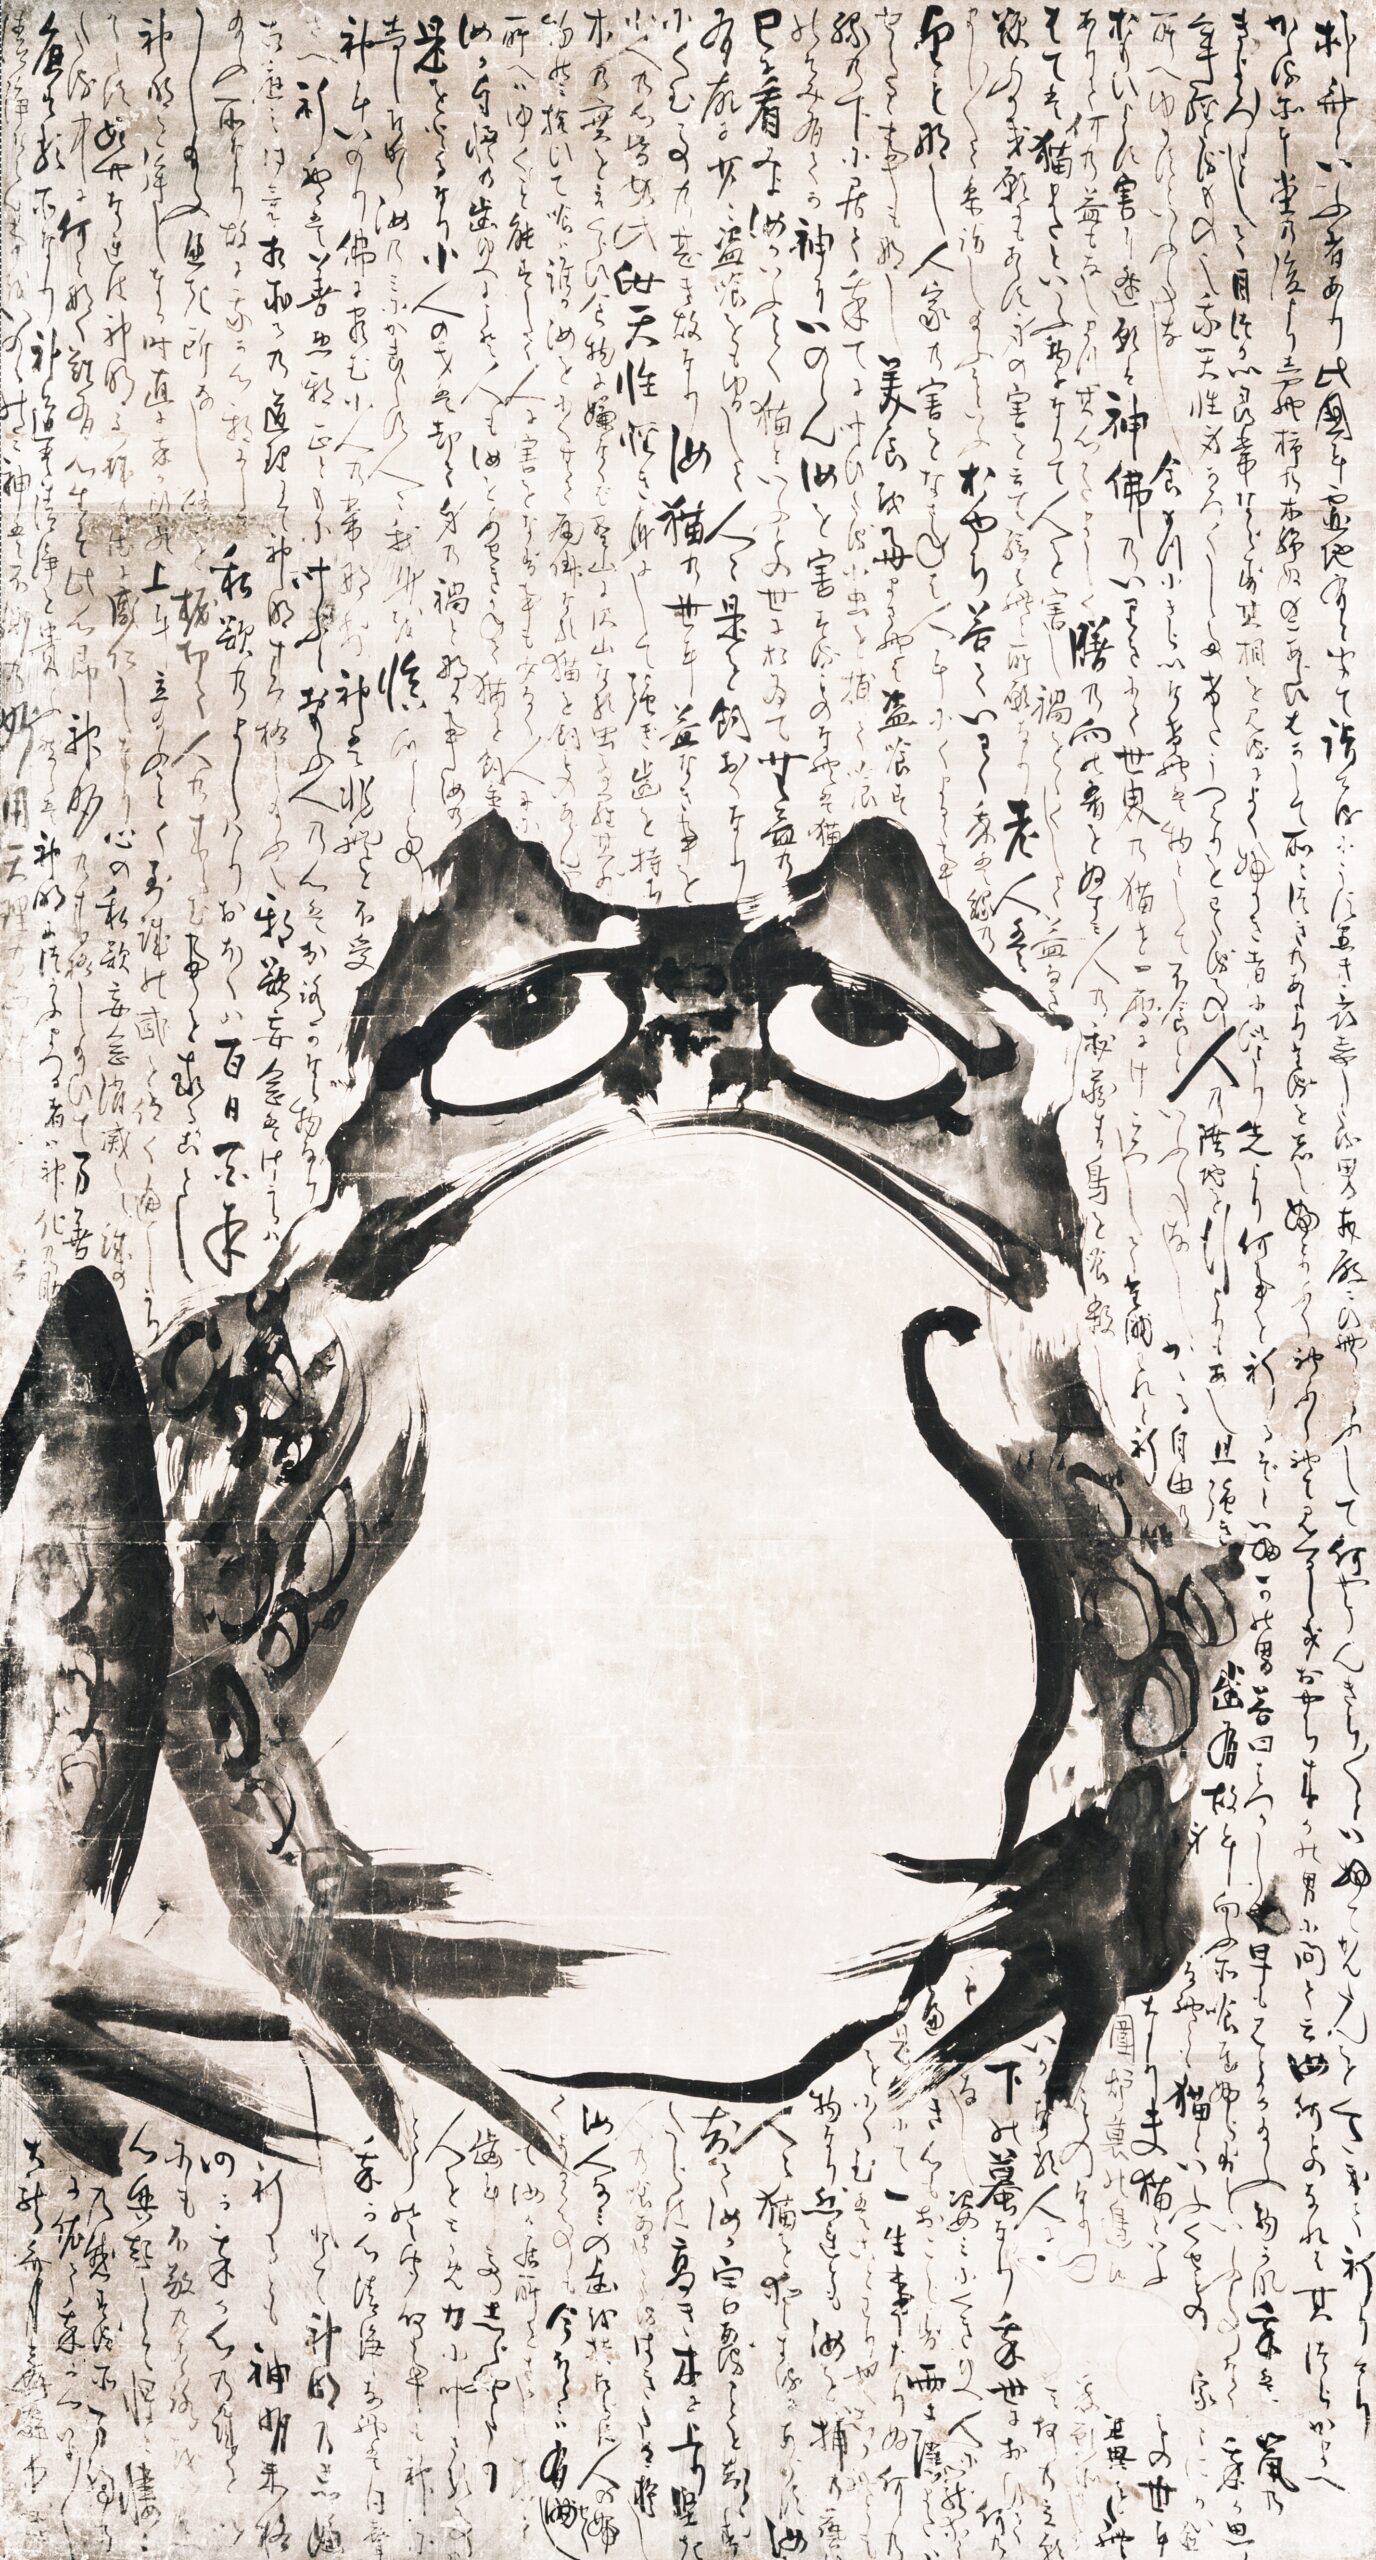
\includegraphics{../img/image13.jpg}

\begin{verseblock}

\newpage

\begin{center}\textbf{61.}\end{center}

要 急 相 應 唯 言 不 二

Yào jí xiāng yìng wéi yán bù èr

Para vivir instantáneamente en armonía con ello,\\
basta decir: no dos.

\end{verseblock}

\hfill\break

\hypertarget{comentario-60}{%
\subsection{Comentario}\label{comentario-60}}

Una mente despierta responde naturalmente a cada circunstancia de manera
adecuada e inmediata, sin necesidad de pasar por las categorías o
distinciones del pensamiento dualista. Esta respuesta surge de la
realización de la no-dualidad, donde no existe separación entre sujeto y
objeto, entre el yo y las demás personas o fenómenos.

Vivir desde el ``no dos'' es actuar con una acción espontánea y
auténtica, alineada con la unidad fundamental de la existencia. En la
tradición budista, enseñamos que cada ser ya posee la naturaleza de
Buda; esta realidad se manifiesta plenamente cuando respondemos al ahora
desde la unidad, libres de dicotomías mentales.

Es esencial reconocer las tendencias kármicas inconscientes que tiñen
nuestra percepción y nuestras reacciones. Estas tendencias, fruto de
hábitos arraigados a lo largo del tiempo, pueden llevarnos a actuar
desde el impulso y la ignorancia en lugar de desde la comprensión
lúcida. El karma no se limita a actos pasados: también moldea las
inclinaciones profundas que determinan nuestra manera de responder al
presente.

Decir ``no dos'' y vivirlo implica estar atentos y atentas a estas
corrientes kármicas, para no ser arrastrados por ellas. Practicamos la
atención plena para reconocer y atravesar nuestros condicionamientos,
permitiendo que nuestra respuesta nazca de la claridad y la unidad
esencial.

Vivir instantáneamente en armonía significa practicar de manera directa,
sin quedar atrapados en construcciones mentales. Es vivir plenamente
despiertos/as en cada instante, frescos y abiertos/as a lo que es,
permitiendo que cada momento nos hable desde su propia verdad, sin
intermediarios.

\hfill\break

\hypertarget{02}{}
\begin{verseblock}

\newpage

\begin{center}\textbf{62.}\end{center}

不 二 皆 同 無 不 包 容

Bù èr jiē tóng wú bù bāo róng

Todo es uno en la no-dualidad,\\
no hay nada que no sea abarcado.

\end{verseblock}

\hfill\break

\hypertarget{comentario-61}{%
\subsection{Comentario}\label{comentario-61}}

Desde la perspectiva de la no-dualidad, no existe separación fundamental
entre las cosas. Todo está contenido en la unidad; nada queda fuera,
nada es ajeno. En este estado de comprensión, cada fenómeno, cada ser,
cada instante, es expresión íntegra de la totalidad.

Si todo es uno, también nosotros y nosotras, en nuestra esencia, somos
todo. Cada ser contiene en sí el potencial infinito de la existencia. Al
mirar el mundo y a nosotros mismos desde este entendimiento, percibimos
la profunda interconexión de nuestros pensamientos, palabras y actos con
todo lo que es.

Nuestra práctica es, entonces, un cultivo de aceptación radical: un
abrirse a la totalidad de la experiencia sin rechazar nada, sin separar
ni discriminar. Pero este camino requiere una vigilancia atenta, porque
las tendencias kármicas inconscientes ---los patrones de rechazo, de
apego, de juicio--- tienden a segregarnos internamente, a fragmentar la
unidad vivida.

Si no reconocemos estas fuerzas sutiles, corremos el riesgo de excluir
partes de nuestra experiencia, atrapados/as en las imágenes limitadas
que nuestro ego ha construido. Y así, nos alejamos de la verdad de
``todo es uno''.

Vivir desde la no-dualidad implica abrazar también nuestras tendencias
más profundas, mirarlas con compasión y sin juicio, permitiéndoles ser
vistas y liberadas. Solo al acogerlo todo ---lo luminoso y lo oscuro, lo
conocido y lo incómodo--- manifestamos plenamente la unidad que somos
realmente. Solo así podemos responder al instante presente con
autenticidad, en comunión con todo lo que es.

\hfill\break

\hypertarget{03}{}
\begin{verseblock}

\newpage

\begin{center}\textbf{63.}\end{center}

十 方 智 者 皆 入 此 宗

Shí fāng zhì zhě jiē rù cĭ zōng

Todos los sabios de las diez direcciones,\\
viven de acuerdo a esta verdad ancestral.

\end{verseblock}

\hfill\break

\hypertarget{comentario-62}{%
\subsection{Comentario}\label{comentario-62}}

El verdadero sabio no es aquel que simplemente acumula conocimientos o
teorías, sino quien ha realizado en su propia vida la verdad profunda de
la existencia. Esta realización no se limita al intelecto: es una
transformación total de la manera de percibir, de sentir y de actuar. En
ella, las fronteras entre sujeto y objeto, entre observador y observado,
se disuelven, dejando solo la unidad viva del momento presente.

Vivir de acuerdo a esta ``verdad ancestral'' no implica alejarse del
mundo o buscar una verdad abstracta fuera de la vida cotidiana. Al
contrario, es integrar la sabiduría en cada gesto, en cada palabra, en
cada pensamiento. No se trata de alcanzar un estado especial apartado de
la existencia diaria, sino de encarnar la comprensión de la naturaleza
interdependiente y vacía de todas las cosas en cada aspecto de la vida.

En la tradición budista, esta sabiduría profunda es llamada prajna: un
saber intuitivo, directo, que atraviesa las apariencias y actúa sin
apego. No es un conocimiento que se posee; es un fluir natural del
despertar en acción.

Así, todos los sabios y sabias de las diez direcciones viven no desde el
esfuerzo de ser sabios, sino desde la naturalidad de haber reconocido y
abrazado la verdad que siempre estuvo presente. La sabiduría no es un
logro final, sino el proceso continuo de despertar, de disolver las
ilusiones, de vivir con compasión y con fidelidad a la realidad tal como
es.

\hfill\break

\hypertarget{04}{}
\begin{verseblock}

\newpage

\begin{center}\textbf{64.}\end{center}

宗 非 促 延 一 念 萬 年

Zōng fēi cù yán yī niàn wàn nián

Esta verdad ancestral no está sujeta a lo breve o lo extenso,\\
en ella un solo instante contiene la eternidad.

\end{verseblock}

\hfill\break

\hypertarget{comentario-63}{%
\subsection{Comentario}\label{comentario-63}}

Para Dogen, el paso del tiempo ---uji (有時), «ser-tiempo»--- no es una
sucesión de instantes que se consumen y desaparecen, ni una línea que
conecta un pasado, un presente y un futuro separados. El tiempo no es
algo exterior que nos afecta, sino la expresión misma de nuestro ser:
ser es ser-tiempo, y cada ser, cada fenómeno, es un momento completo que
contiene en sí la totalidad de la existencia.

La verdad ancestral no está sujeta a medidas humanas como lo breve o lo
extenso. No puede reducirse a un intervalo de segundos ni abarcarse en
millones de años. En esta verdad, cada instante ---por pequeño o fugaz
que nos parezca--- es absoluto. Cada ahora contiene la eternidad. No
porque dure para siempre, sino porque en su propia naturaleza es
intemporal: no viene de ningún lugar ni se dirige hacia ningún destino.

Cuando nos sentamos en zazen, no lo hacemos para avanzar hacia un logro
futuro. Sentarse, respirar, ser conscientes en este instante es ya
manifestar el despertar. Practicar zazen es entrar en contacto con esta
dimensión profunda donde el tiempo lineal se desvanece, y solo queda la
presencia viva e ilimitada de cada momento. No practicamos para ser
mejores más adelante, sino para vivir plenamente este ahora, donde todo
se encuentra reunido.

Para Dogen «la práctica y la realización son uno». No existe separación
entre el camino y la meta. De igual modo, no hay necesidad de buscar
otra vida, otro momento, otro estado. Cada instante de vida, vivido con
atención y entrega, contiene los «diez mil mundos». Este ahora, que
parece tan breve y frágil, es, en verdad, el despliegue completo del
universo entero.

En la práctica cotidiana, podemos olvidar esta dimensión y quedar
atrapados en la ilusión de que el tiempo se nos escapa o nos empuja.
Volver a la presencia ---al simple hecho de estar aquí, respirando,
sintiendo, siendo--- es recordar que no somos arrastrados por el tiempo,
sino que somos tiempo, somos este momento completo.

Por eso en la verdad ancestral no hay «venir» ni «ir». No nacemos ni
morimos en un sentido absoluto: simplemente somos expresión de este
fluir eterno que no necesita transcurrir para ser. Cada paso, cada
mirada, cada respiración puede convertirse en un portal hacia esta
eternidad siempre disponible.

Habitar plenamente cada instante es abrazar la eternidad que somos. No
como una idea, sino como una experiencia viva, que disuelve las
fronteras entre nosotros/as y el mundo, entre ahora y siempre, entre ser
y tiempo.

\hfill\break

\hypertarget{05}{}
\begin{verseblock}

\newpage

\begin{center}\textbf{65.}\end{center}

無 在 不 在 十 方 目 前

Wú zài bù zài shí fāng mù qián

Más allá del ser y del no ser,\\
se manifiesta en todas partes.

\end{verseblock}

\hfill\break

\hypertarget{comentario-64}{%
\subsection{Comentario}\label{comentario-64}}

Nada existe de manera independiente ni posee una esencia fija. Todo lo
que percibimos es vacío: vacío de identidad propia. Sin embargo, esta
vacuidad no debe confundirse con la no existencia o con un vacío
nihilista. Las cosas son reales en tanto que surgen
interdependientemente, en un flujo constante de relaciones que no dejan
lugar a un ser aislado ni a un no ser absoluto.

La realidad ---la talidad (tathatā)--- no es algo separado o lejano. No
es un estado oculto reservado a unos pocos, ni una verdad que aparece
sólo en circunstancias especiales. Se manifiesta en todas partes, en
cada instante, en cada encuentro, en cada respiración. Toda la realidad
se despliega siempre, aquí y ahora, más allá de toda categoría que trate
de encajonarla en ``ser'' o ``no ser''.

En zazen, soltamos el impulso de atrapar la experiencia en conceptos. No
afirmamos ni negamos; simplemente nos abrimos a lo que es. Y en esa
apertura, se revela la naturaleza verdadera de las cosas: ni existencia
fija ni aniquilación, sino presencia viva, fluida, sin borde ni centro.
Una realidad que no puede ser poseída ni delimitada, pero que puede ser
vivida directamente.

Más allá de las palabras, más allá de las ideas de existir o no existir,
esta presencia se manifiesta silenciosamente en todas partes. Es la taza
que levantamos, la brisa que acaricia el rostro, el sonido de una
campana a lo lejos. No hay necesidad de buscarla: ya está aquí, siempre
disponible, delante de nuestros ojos, esperando ser reconocida en la
sencillez de cada momento.

\hfill\break

\begin{center}\rule{0.5\linewidth}{0.5pt}\end{center}

\hfill\break

\hypertarget{01}{}
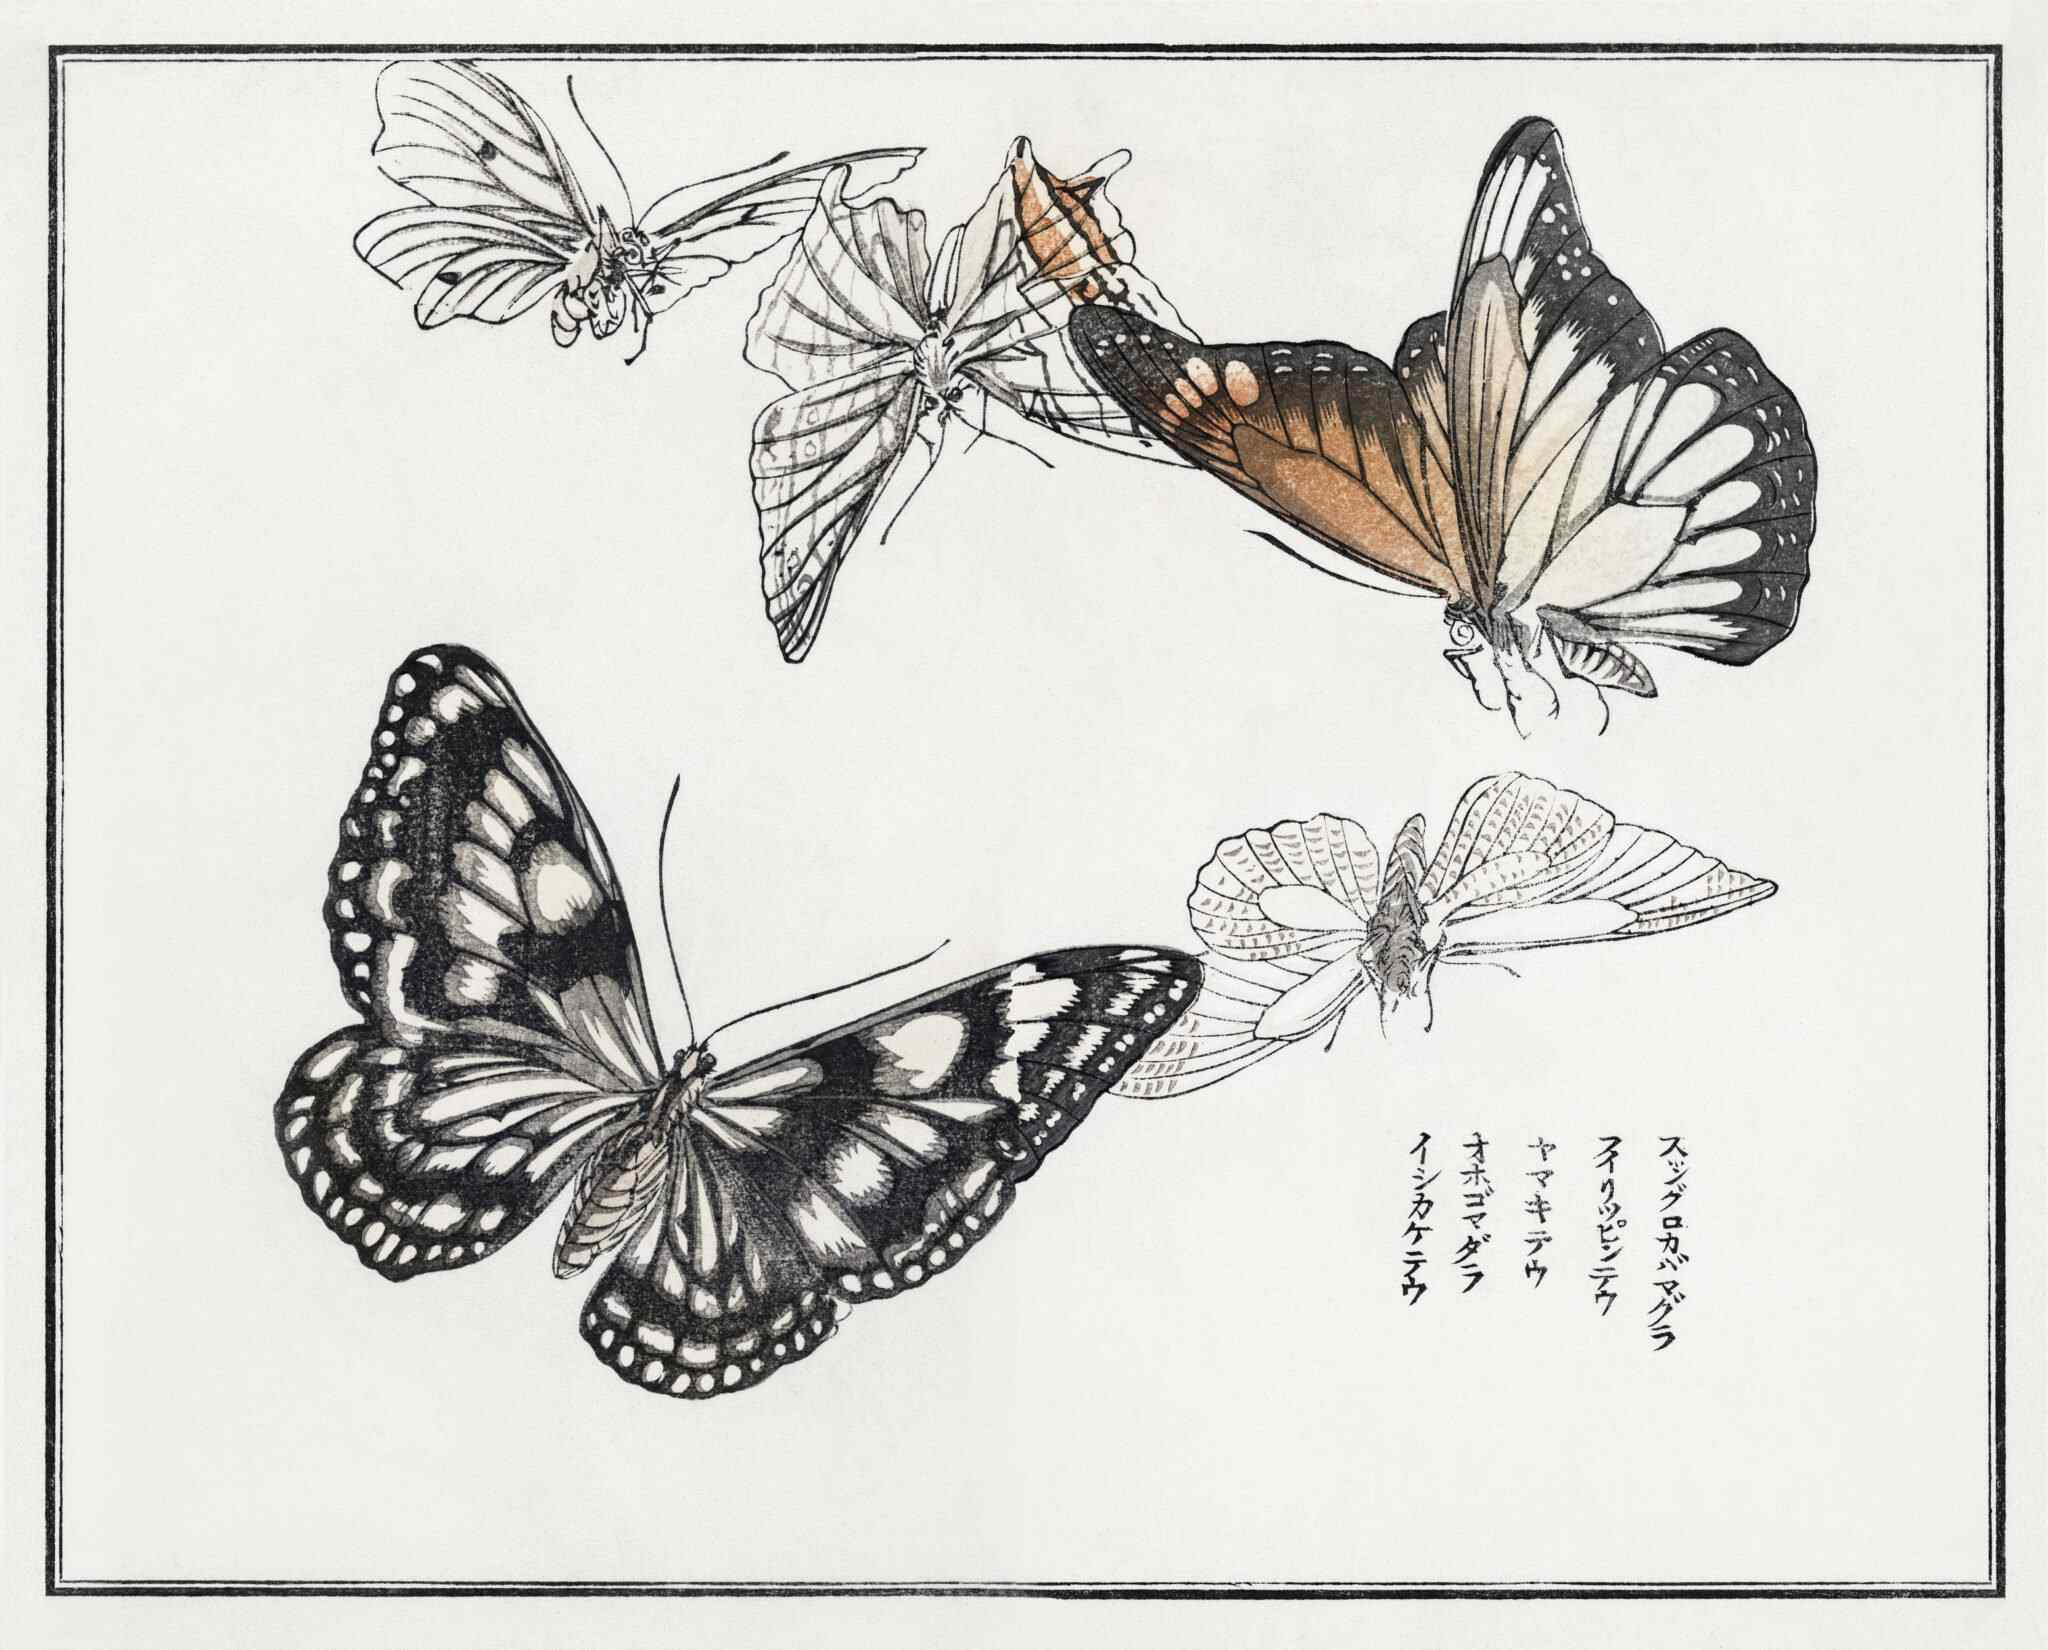
\includegraphics{../img/image14.jpg}

\begin{verseblock}

\newpage

\begin{center}\textbf{66.}\end{center}

極 小 同 大 忘 絶 境 界

Jí xiăo tong dà Wàng jué jìng jiè

Lo infinitamente pequeño es idéntico a lo infinitamente grande,\\
cuando se olvidan los límites y se disuelven las fronteras.

\end{verseblock}

\hfill\break

\hypertarget{comentario-65}{%
\subsection{Comentario}\label{comentario-65}}

Los conceptos no son más que construcciones mentales que nos mantienen
atrapados/as en una visión fragmentada de la realidad. En la experiencia
directa de la práctica, estas distinciones pierden su solidez. Una hoja,
una montaña, un átomo o el universo entero son manifestaciones de la
misma realidad fundamental, entretejidas en una red de interdependencia
que trasciende nuestras categorías habituales.

En zazen, emerge naturalmente una percepción profunda de la realidad. Lo
pequeño y lo grande, lo interno y lo externo, lo uno y lo múltiple,
coexisten y se interpenetran más allá de los límites que el pensamiento
impone. No es que lo pequeño se convierta en grande o lo grande en
pequeño, sino que ambos, en su verdadera naturaleza, dejan de ser
opuestos.

Esta experiencia de interpenetración se despliega en samadhi: un estado
donde las fronteras entre uno mismo y el mundo se disuelven, donde ya no
hay un adentro ni un afuera separados. Al ``olvidar'' los límites ---es
decir, al no fijar la atención en ellos--- permitimos que la unidad
subyacente se manifieste de forma viva. Así, lo pequeño contiene lo
grande, y lo grande se refleja plenamente en lo pequeño, sin conflicto
ni separación.

Dogen expresa esta verdad de manera poética en el
Genjōkōan\textsuperscript{\protect\hypertarget{ref1}{\protect\hyperlink{nota1}{1}}}:

"Cuando el ser humano realiza el despertar es como el reflejo de luna en
el agua. La luna se refleja en el agua pero no se moja, el agua no se
agita por este reflejo.

La luz de la luna ilumina hasta el infinito. Ilumina toda la Tierra. Por
amplia y vasta que sea su luz puede ser contenida en la mínima gota de
rocío.

Así como la luna no agita el agua, el despertar tampoco es un obstáculo
para el ser humano. El ser humano no pone más obstáculos al despertar
que la gota de rocío a la luna o al cielo.

La profundidad de la realización es proporcional a la altura de la luna.
La profundidad de la gota de rocío puede contener las alturas de la luna
y el cielo."

Esta enseñanza señala que, en la visión verdadera, no hay diferencia de
rango ni de tamaño: cada instante, cada fenómeno, cada ser refleja
íntegramente la vastedad de la existencia. La gota de rocío no disminuye
la inmensidad del cielo ni la luna se pierde en el reflejo. Así también
nosotros/as, cuando soltamos las fronteras de la mente, podemos ver que
lo infinito habita en lo más pequeño, y que cada manifestación
particular contiene la totalidad.

\hfill\break

\hypertarget{02}{}
\begin{verseblock}

\newpage

\begin{center}\textbf{67.}\end{center}

極 大 同 小 不 見 邊 表

Jí dà tóng xiăo bù jiàn biān biăo

Lo infinitamente grande es idéntico a lo infinitamente pequeño,\\
los límites y las apariencias se desvanecen.

\end{verseblock}

\hfill\break

\hypertarget{comentario-66}{%
\subsection{Comentario}\label{comentario-66}}

Nuestra visión del mundo está condicionada por los límites de nuestros
sentidos, así como por los filtros de la cultura, la educación y las
experiencias personales. Así como una persona habituada a los paisajes
nevados puede distinguir matices en la nieve que otros pasan por alto,
también nosotros/as, moldeados por nuestro aprendizaje y nuestra
práctica, solo alcanzamos a percibir una fracción de la vastedad de la
realidad.

Vemos aquello que nuestros ojos, apoyados en nuestra sensibilidad y
comprensión, son capaces de captar. La profundidad de nuestra percepción
depende del grado de apertura que hayamos cultivado en nuestro corazón y
nuestra mente. Sin embargo, incluso lo que creemos ver o entender son
apenas reflejos parciales de una totalidad inconmensurable.

Cuando clasificamos la realidad en categorías como "grande" o "pequeño",
"importante" o "insignificante", solo estamos elaborando
interpretaciones basadas en nuestro punto de vista limitado. Más allá de
estas divisiones, lo infinitamente grande y lo infinitamente pequeño no
son opuestos: se reflejan mutuamente, se interpenetran, son
manifestaciones de una única y misma realidad.

Así como en el océano hay características que escapan a nuestra
observación y existen innumerables montañas invisibles a nuestros ojos,
también hay mundos, dimensiones y niveles de experiencia que transcurren
más allá de nuestras concepciones habituales. El ojo condicionado ve
fragmentos; la realidad plena permanece, siempre, más vasta de lo que
cualquier fragmento puede contener.

Expandir nuestra mirada no es cuestión de acumular nuevas categorías,
sino de soltarlas todas. Es descubrir que cada grano de arena contiene
todos los océanos, y que la totalidad del cielo puede habitar una sola
gota de rocío.

\hfill\break

\hypertarget{03}{}
\begin{verseblock}

\newpage

\begin{center}\textbf{68.}\end{center}

有 即 是 無 無 即 是 有

Yŏu jí shì wú Wú jí shì yŏu

El ser es, en sí mismo, no-ser,\\
el no-ser es, en sí mismo, ser.

\end{verseblock}

\hfill\break

\hypertarget{comentario-67}{%
\subsection{Comentario}\label{comentario-67}}

En la tradición Zen, distinciones como «ser» (u) y «no-ser» (mu) no son
polos enfrentados, sino manifestaciones inseparables de una misma
realidad viva. Todo aquello que aparece como «ser» carece de esencia
fija, es vacío (śūnyatā), y es precisamente este vacío lo que permite su
surgimiento y su transformación constante. Del mismo modo, el «no-ser»
no implica una negación absoluta, sino una dimensión que hace posible el
fluir y la renovación de la existencia.

Cada instante se despliega como ser y no-ser entrelazados: nacer y
desaparecer, formar y disolver, sin ruptura ni separación. La vida no es
algo que se afirma contra el vacío, ni el vacío algo que niega la vida.
Son uno.

En la práctica de zazen, esta unidad más allá de los opuestos se
encarna. Sentarse no es buscar afirmar el yo ni disolverlo en la nada.
No se trata de alcanzar un estado de «ser algo» ni de «no ser nada».
Zazen es simplemente estar, más allá de toda categoría, en la frescura
del instante en que ser y no-ser se reflejan mutuamente.

El maestro Dogen expresa esta experiencia con la frase «shinjin
datsuraku» ---``abandono de cuerpo y mente''---, señalando el acto de
soltar completamente todas las fijaciones: soltar las ideas sobre el
cuerpo y la mente, sobre el ser y el no-ser, sobre la práctica y la
realización. No es aniquilación, ni indiferencia, sino un dejar caer
espontáneo, natural, en el que la existencia se vive tal cual es, libre
de los esquemas conceptuales que la fragmentan.

Cuando cesa la lucha por afirmar o negar, se revela una libertad más
allá del pensamiento: una intimidad profunda, no fabricada, con todo lo
que es.

Así, vivir esta unidad no es una abstracción filosófica, sino un modo de
estar plenamente vivos/as, abiertos/as al flujo continuo en el que ser y
no-ser son simplemente expresiones de una misma vida indivisible.

\hfill\break

\hypertarget{04}{}
\begin{verseblock}

\newpage

\begin{center}\textbf{69.}\end{center}

若 不 如 此 必 不 須 守

Ruò bù rú cĭ bì bù xū shŏu

Si no es así,\\
entonces no hay necesidad de aferrarse.

\end{verseblock}

\hfill\break

\hypertarget{comentario-68}{%
\subsection{Comentario}\label{comentario-68}}

Si no comprendemos la verdadera naturaleza de la existencia ---abierta,
fluida, sin esencia fija--- nos veremos inevitablemente atrapados en el
impulso de aferrarnos. Aferrarnos a las formas, a las ideas, a la
identidad. Pero todo aquello que intentamos retener está ya en proceso
de transformación; nada permanece, nada puede ser poseído.

Cuando se reconoce íntimamente que la realidad no puede ser fijada ni
encerrada, la necesidad de aferrarse se desvanece por sí misma. No hay
esfuerzo por soltar: simplemente no hay a qué aferrarse.

En zazen, sentarse sin aspiración ni rechazo es entrar en contacto
directo con esta verdad. No buscamos solidificar el yo, ni buscamos
anularlo. No hay lucha. El instante se revela completo, tal como es, sin
necesidad de intervención.

Aferrarse nace de la ilusión de separación; no-aferrarse nace de la
experiencia de unidad. Allí donde cesa el deseo de retener o resistir,
brota una libertad silenciosa, una intimidad sin barreras con todo lo
que surge y se desvanece.

No se trata de abandonar el mundo, sino de habitarlo de otra manera: con
los ojos abiertos, las manos abiertas, el corazón abierto. Al comprender
que no hay nada permanente a lo que agarrarse, la vida entera se
convierte en una expresión natural de la Vía.

\hfill\break

\hypertarget{05}{}
\begin{verseblock}

\newpage

\begin{center}\textbf{70.}\end{center}

一 即 一 切 一 切 即 一

Yī jí yī qiè yī qiè jí yī

Uno es todo.\\
Todo es uno.

\end{verseblock}

\hfill\break

\hypertarget{comentario-69}{%
\subsection{Comentario}\label{comentario-69}}

Hay una interconexión profunda entre lo particular y lo universal, entre
lo relativo y lo absoluto. Cada fenómeno individual contiene la
totalidad del cosmos, y el cosmos se manifiesta plenamente en cada cosa.
Esta comprensión disuelve la ilusión de separación, revelando una
realidad donde lo absoluto y lo relativo coexisten inseparablemente. En
el zazen, esta unidad se experimenta directamente, mostrando que el «yo»
no está aislado, eso es solo una ilusión compartida, ya que forma parte
de un todo dinámico e interdependiente.

No se trata solo de comprender intelectualmente, sino de darnos cuenta
de que existen distintas formas de experimentar el mundo. Podemos ver
cada cosa como algo independiente, o como expresión de la totalidad. Lo
importante es poder movernos libremente entre estas perspectivas,
respondiendo adecuadamente según las circunstancias. Esta capacidad de
adaptarse, de pasar del uno al todo y del todo al uno, es lo que permite
una vida armoniosa, en sintonía con la realidad cambiante.

Cada momento y cada acción son una oportunidad para expresar esta
comprensión, actuando con compasión y sabiduría. Al vivir desde esta
libertad, nuestras acciones no solo reflejan la conexión con el todo,
sino que responden de manera precisa y creativa a las demandas del
momento presente.

\hfill\break

\begin{center}\rule{0.5\linewidth}{0.5pt}\end{center}

\leavevmode\vadjust pre{\hypertarget{notas}{}}%
\textsuperscript{1} Texto completo
https://zendogen.es/textos/shobogenzo/genjokoan/
\protect\hyperlink{ref1}{Volver}

\hfill\break

\hypertarget{01}{}
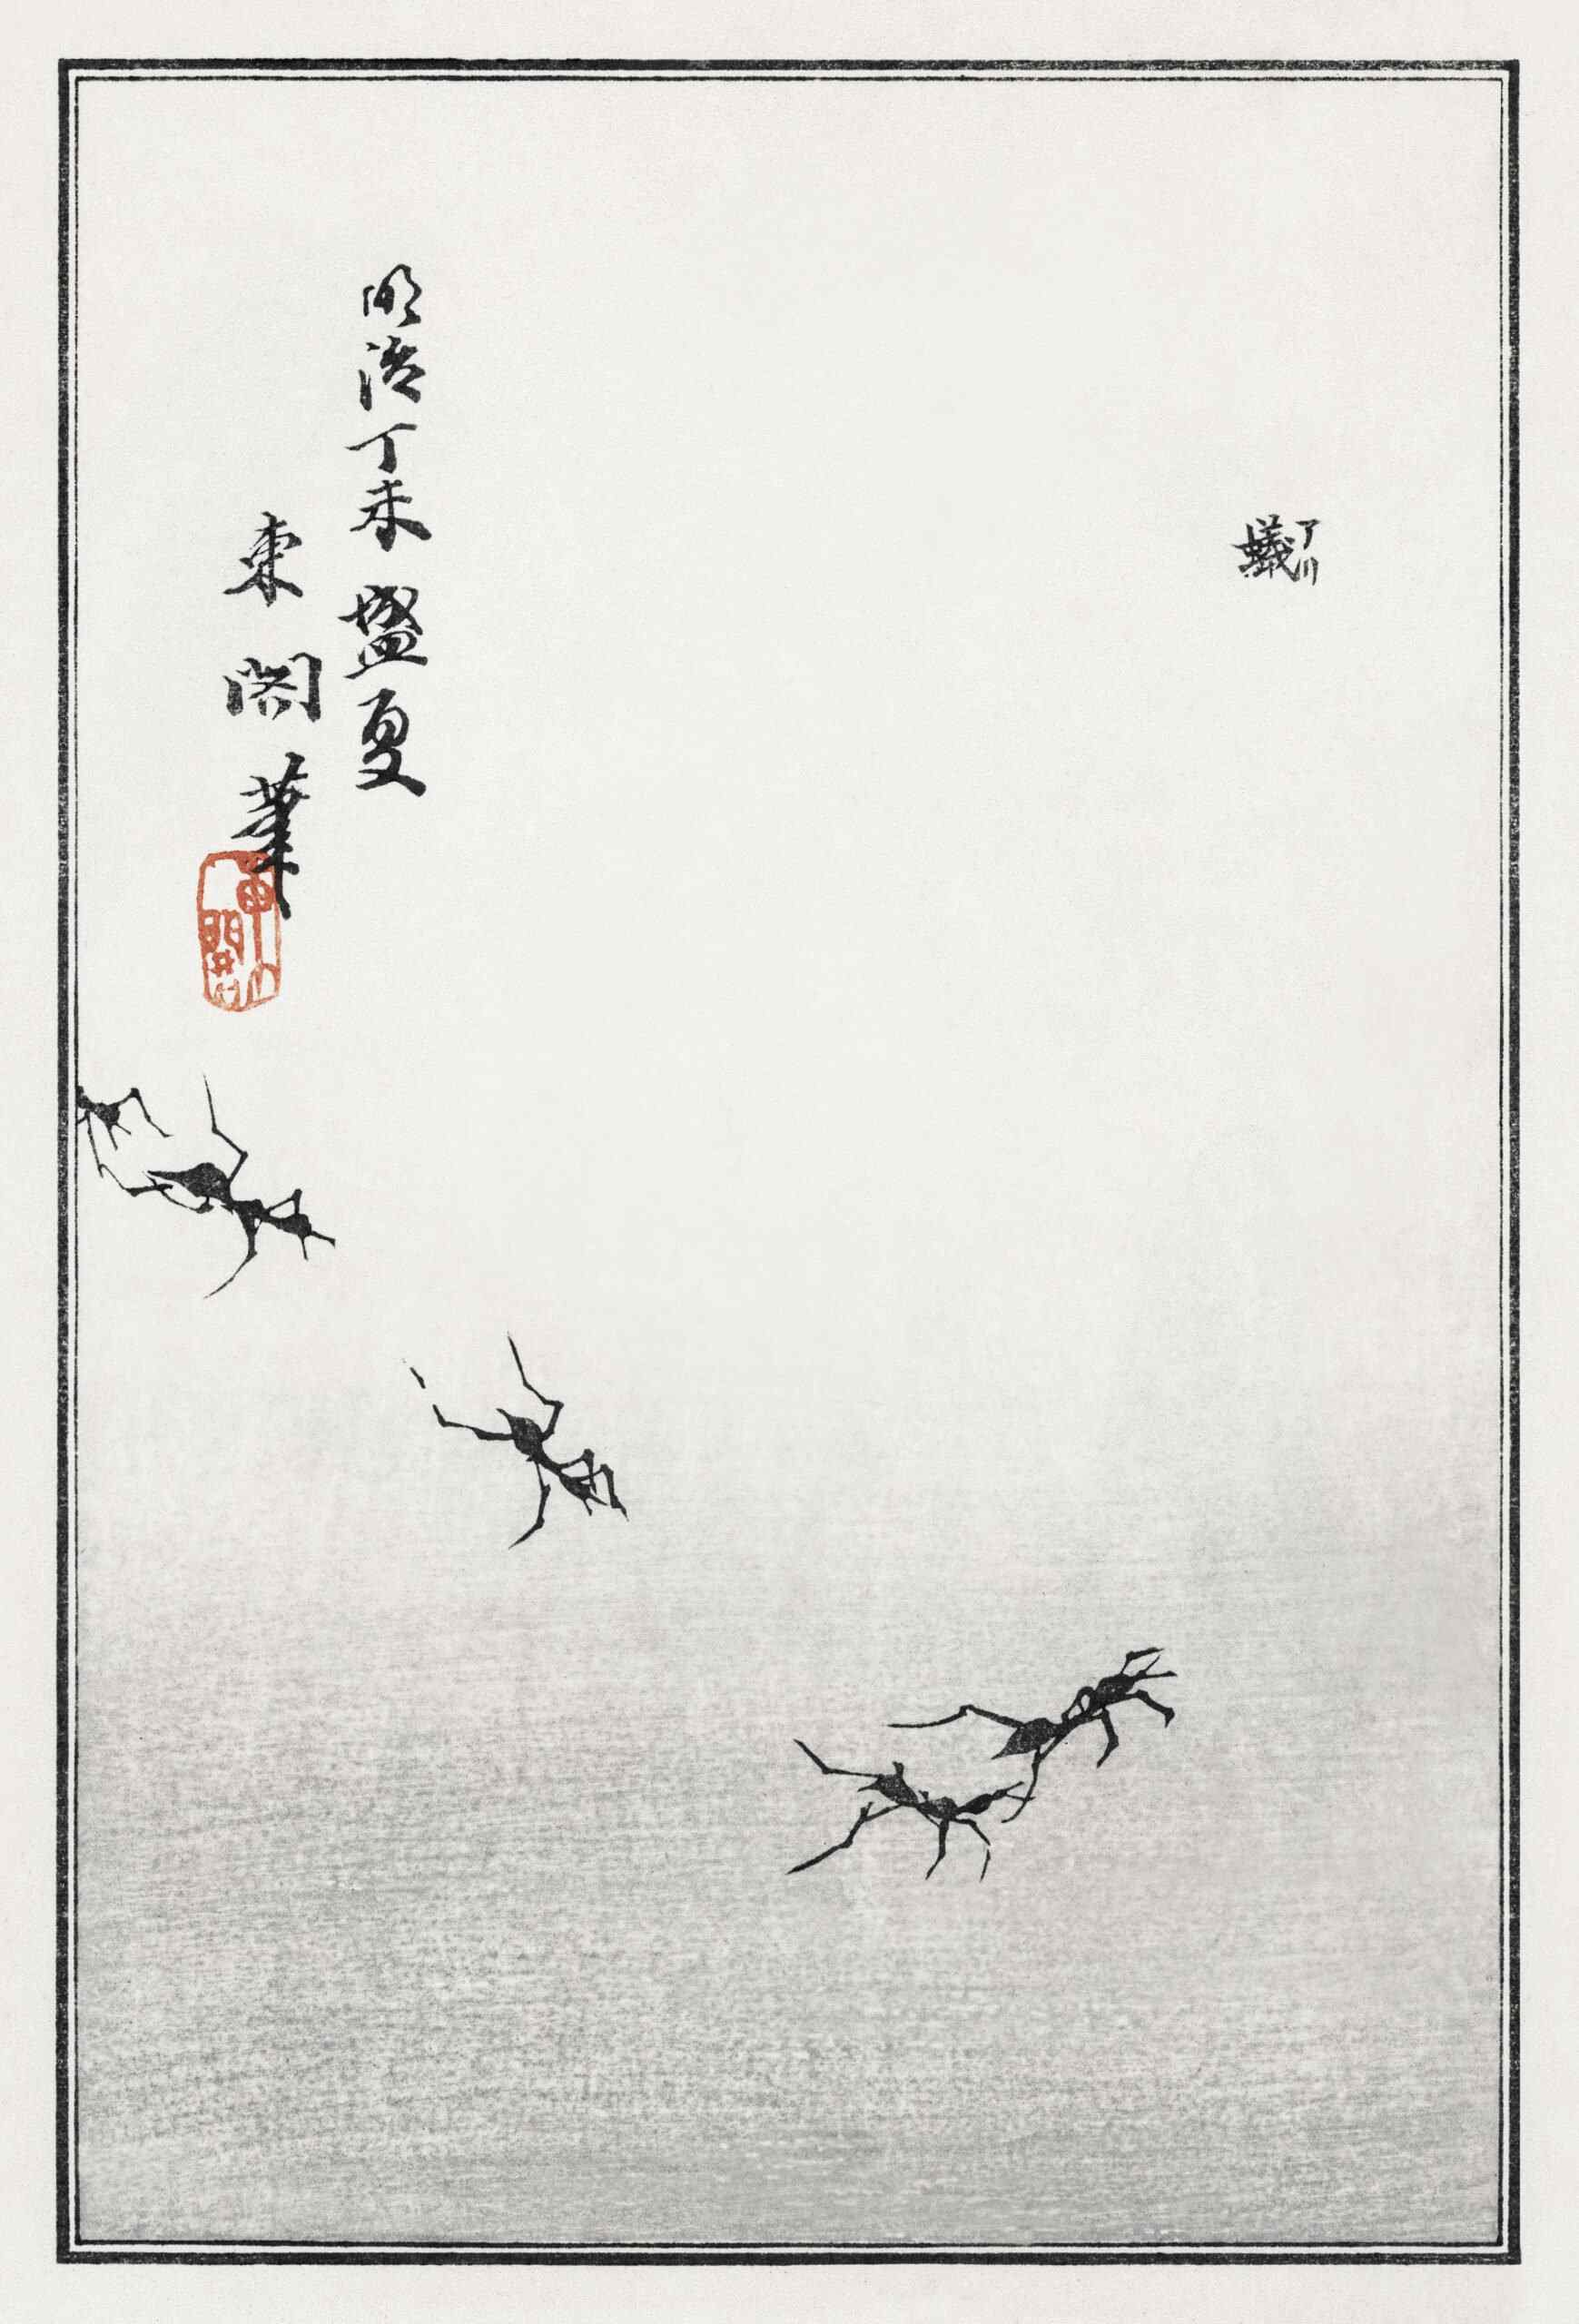
\includegraphics{../img/image15.jpg}

\begin{verseblock}

\newpage

\begin{center}\textbf{71.}\end{center}

但 能 如 是 何 慮 不 畢

Dàn néng rú shì hé lü bù bì

Si puedes ser así,\\
no hay motivo para inquietarse por el resultado.

\end{verseblock}

\hfill\break

\hypertarget{comentario-70}{%
\subsection{Comentario}\label{comentario-70}}

La realidad es tal como es: en su despliegue inmediato, cada instante
contiene la plenitud de lo que necesitamos. No hay nada que añadir ni
nada que quitar. En la naturaleza cambiante de la existencia, cada
momento es completo en sí mismo, sin depender de futuros resultados ni
de logros pendientes.

Cuando, a través de la práctica, buscamos algo separado o distante, nos
alejamos de la vivencia directa del ahora. La mente se extravía en
conceptualizaciones, aspiraciones y deseos de alcanzar un estado mejor,
perdiendo la riqueza silenciosa del instante presente.

Si podemos asentarnos en este momento tal como es, sin perseguir ni
rechazar, no hay motivo para inquietarse. No es necesario abarcar lo
infinito, porque lo infinito se manifiesta plenamente en cada
respiración, en cada paso, en cada mirada sencilla. La actitud a
cultivar no es controlar, poseer o entenderlo todo desde el intelecto,
sino confiar en la interdependencia viva de la realidad y actuar con la
serenidad de quien sabe que cada cosa encuentra su lugar naturalmente.

Cuando dejamos de lado nuestras inquietudes, nuestros cálculos y
nuestros miedos, nos alineamos con la existencia. Vivir desde esta
confianza no es pasividad, sino una forma activa de sabiduría: implica
estar disponibles y abiertos/as a cada situación, respondiendo
creativamente a las necesidades del momento, sin rigidez ni expectativas
ilusorias.

Al reconocer que no necesitamos fabricar ningún resultado especial, la
ansiedad se disuelve, y la vida misma se convierte en una danza de
presencia y libertad, donde lo infinito se actualiza instante tras
instante en el corazón mismo de lo que somos.

\hfill\break

\hypertarget{02}{}
\begin{verseblock}

\newpage

\begin{center}\textbf{72.}\end{center}

信 心 不 二 不 二 信 心

Xìn xīn bù èr Bù èr xìn xīn

La esencia de la confianza es no-dualidad.\\
No-dualidad es la esencia de la confianza.

\end{verseblock}

\hfill\break

\hypertarget{comentario-71}{%
\subsection{Comentario}\label{comentario-71}}

Confiar es vivir sin dividir. La confianza profunda nace cuando dejamos
de vernos separados del mundo, cuando soltamos la percepción del ``yo''
por un lado, y ``todo lo demás'' por otro. La mente condicionada,
atrapada en el hábito de distinguir entre dentro y fuera, mío y no mío,
nos mantiene en una sensación constante de distancia y lucha. Pero
cuando dejamos caer estas barreras, nos encontramos con algo que siempre
estuvo ahí: nuestra naturaleza original, plena, viva, completa.

En esa experiencia de no-dualidad, la confianza surge sola. No es algo
que fabriquemos, ni una creencia a la que nos aferremos. Es como
respirar: natural, sencillo, inevitable. Confiamos porque sentimos, de
forma directa, que no estamos separados de la vida. Esta confianza no
depende de que todo salga como queremos. No necesita promesas ni
seguridades. Es el reconocimiento íntimo de que, pase lo que pase, la
vida misma nos sostiene.

Cuando descansamos en esta confianza, dejamos de luchar contra la
corriente de la existencia y ya no sentimos la necesidad de controlar o
resistirnos. Vivimos abiertos/as, atentos/as, disponibles para cada
momento, con la sabiduría de saber que cada paso, incluso el incierto,
forma parte de un camino mayor que nos incluye y nos nutre.

La práctica de zazen nos ayuda a integrar esta enseñanza como una
experiencia viva. Nos enseña a soltar las viejas armaduras que nos
separan del mundo. Cuando experimentamos que en el fondo no hay dos, que
la vida y nosotros/as somos uno, confiar se vuelve algo natural.
Entonces, saltar al vacío de lo desconocido, deja de ser aterrador.
Descubrimos que siempre hemos estado en casa, que no hay nada a lo que
llegar.

Esta confianza serena transforma nuestra manera de estar en el mundo.
Nos permite vivir con más coraje, más alegría, más autenticidad. Nos
enseña que podemos caminar, respirar, amar y soltar... sabiendo que
siempre estamos sostenidos/as.

\hfill\break

\hypertarget{03}{}
\begin{verseblock}

\newpage

\begin{center}\textbf{73.}\end{center}

言 語 道 斷 非 去 來 今

Yán yŭ dào duàn fēi qù lái jīn

Una vez aquí el lenguaje se silencia,\\
y el pasado, el futuro y el presente desaparecen.

\end{verseblock}

\hfill\break

\hypertarget{comentario-72}{%
\subsection{Comentario}\label{comentario-72}}

El despertar trasciende el lenguaje y el tiempo. El lenguaje no puede
captar la realidad tal cual es. En el buddhadharma, las palabras son
solo herramientas temporales que no pueden abarcar lo inefable. Solo
cuando cesan los conceptos y las explicaciones, se abre el espacio para
experimentar directamente lo que es, sin necesidad de intermediarios.

La realidad no es algo que pueda explicarse con palabras, sino algo que
se vive plenamente cuando soltamos la mente discursiva a través de la
experiencia directa. En nuestra tradición, a través de la práctica de
zazen accedemos a este silencio que está más allá de las palabras y el
silencio, las categorías de pasado, futuro y presente pierden su
significado, y lo que queda es simplemente estar aquí, más allá de todo
concepto, en una paz que no necesita explicaciones.

La realidad no se puede fragmentar en pasado, presente y futuro; no es
un punto fijo que podamos localizar ni un instante que podamos poseer.
Tiempo y ser son inseparables, como expresa Dogen en el Shôbôgenzô en el
capítulo uji, ser-tiempo, donde manifiesta que cada momento contiene la
totalidad del ser. Cuando observamos una gota de agua caer, no es solo
``una gota en un instante''. Es la culminación de todo lo que permitió
que existiera: la nube, la lluvia, la tierra, el sol. Esa gota contiene
el universo entero, porque sin el universo, no podría ser. De igual
forma, cada instante contiene la totalidad del ser, porque no hay
separación entre lo que somos, lo que hacemos y el momento en que
sucede.

Esta comprensión no se alcanza buscando fuera ni aferrándose a
categorías mentales, sino abandonando las estructuras que condicionan
nuestra percepción y permitiendo que la experiencia fluya libremente,
sin límites impuestos por la mente discursiva. Viviendo plenamente cada
instante, sabiendo que no es un paso hacia otro lugar o momento, sino la
totalidad misma de la existencia, manifestándose aquí y ahora.

Debemos soltar no solo el lenguaje y las nociones de tiempo, sino
también la insistencia en definir y controlar la experiencia. El camino
del zen no es un medio para alcanzar un estado futuro, sino la
manifestación directa del despertar aquí y ahora. En este estar
completamente presentes, el ``yo'' desaparece, las barreras se
disuelven, y lo que queda es la plena expresión de la vida tal como es,
completa y perfecta en sí misma.

\hfill\break

\newpage

\begin{center}\textbf{Traducción del Xin Xin Ming}\end{center}

\hypertarget{a-continuaciuxf3n-el-xin-xin-ming-en-su-forma-original-incluyendo-el-texto-en-chino-ux6f22ux5b57-su-transcripciuxf3n-en-pinyin-y-su-traducciuxf3n-al-castellano-verso-a-verso.-se-ha-procurado-mantener-la-claridad-y-la-precisiuxf3n-respetando-el-espuxedritu-del-poema-sin-perder-su-profundidad.}{%
\subparagraph{A continuación el Xin Xin Ming en su forma original,
incluyendo el texto en chino (漢字), su transcripción en pinyin y su
traducción al castellano, verso a verso. Se ha procurado mantener la
claridad y la precisión, respetando el espíritu del poema sin perder su
profundidad.}\label{a-continuaciuxf3n-el-xin-xin-ming-en-su-forma-original-incluyendo-el-texto-en-chino-ux6f22ux5b57-su-transcripciuxf3n-en-pinyin-y-su-traducciuxf3n-al-castellano-verso-a-verso.-se-ha-procurado-mantener-la-claridad-y-la-precisiuxf3n-respetando-el-espuxedritu-del-poema-sin-perder-su-profundidad.}}

Xin Xin Ming

Tratado sobre la Confianza en la Naturaleza Original

\begin{verseblock}

\hypertarget{section-75}{%
\subsection{1.}\label{section-75}}

至 道 無 難 唯 嫌 揀 擇

Zhì dào wù nán Wéi xián jiăn zé

La realización del Gran Despertar no es difícil,\\
tan solo evita el apego y el rechazo.

\end{verseblock}

\begin{verseblock}

\hypertarget{section-76}{%
\subsection{2.}\label{section-76}}

但 莫 憎 愛 洞 然 明 白

Dàn mò zēng ài dòng rán míng bái

Cuando no aparece el apego ni el rechazo,\\
todo manifiesta su naturaleza luminosa.

\end{verseblock}

\begin{verseblock}

\hypertarget{section-77}{%
\subsection{3.}\label{section-77}}

毫 釐 有 差 天 地 懸 隔

Háo lí yŏu chā tiān dì xuán gé

Si aparece la más mínima diferencia,\\
cielo y tierra quedan separados por un abismo.

\end{verseblock}

\begin{verseblock}

\hypertarget{section-78}{%
\subsection{4.}\label{section-78}}

欲 得 現 前 莫 存 順 逆

Yù dé xiàn qián, mò cún shùn nì.

Si deseas ver la verdad ante ti,\\
no tomes partido a favor ni en contra de nada.

\end{verseblock}

\begin{verseblock}

\hypertarget{section-79}{%
\subsection{5.}\label{section-79}}

違 順 相 爭 是 爲 心 病

Wéi shùn xiāng zhēng, shì wèi xīn bìng

El conflicto entre lo que aceptas y lo que rechazas,\\
enferma el corazón y la mente.

\end{verseblock}

\begin{verseblock}

\hypertarget{section-80}{%
\subsection{6.}\label{section-80}}

不 識 玄 旨 徒 勞 念 靜

Bù shí xuán zhĭ tú láo niàn jìng

Si no comprendes el principio profundo,\\
te esfuerzas en vano en buscar la quietud.

\end{verseblock}

\begin{verseblock}

\hypertarget{section-81}{%
\subsection{7.}\label{section-81}}

圓 同 太 虚 無 欠 無 餘

Yuán tóng tài xŭ wú qiàn, wú yú

Plena como el gran vacío,\\
nada falta, nada sobra.

\end{verseblock}

\begin{verseblock}

\hypertarget{section-82}{%
\subsection{8.}\label{section-82}}

良 由 取 捨 所 以 不 如

Liáng yóu qŭ shě suŏ yĭ bù rú

Es precisamente por aferrarnos y rechazar,\\
que perdemos nuestra armonía natural.

\end{verseblock}

\begin{verseblock}

\hypertarget{section-83}{%
\subsection{9.}\label{section-83}}

莫 逐 有 縁 勿 住 空 忍

Mò zhú yŏu yuán wù zhù kōng rěn

No persigas lo que surge de los fenómenos.\\
ni te aferres a la vacuidad.

\end{verseblock}

\begin{verseblock}

\hypertarget{section-84}{%
\subsection{10.}\label{section-84}}

一 種 平 懷 泯 然 自 盡

Yī zhŏng ping huái mĭn rán zì jìn

Cultiva una mente y un corazón ecuánimes,\\
y la dualidad desaparecerá por sí misma.

\end{verseblock}

\begin{verseblock}

\hypertarget{section-85}{%
\subsection{11.}\label{section-85}}

止 動 歸 止 止 更 彌 動

Zhĭ dòng guī zhĭ zhĭ gèng mí dòng

Intentar detener el movimiento solo lo intensifica aún más,\\
cuando el movimiento cesa, la calma regresa.

\end{verseblock}

\begin{verseblock}

\hypertarget{section-86}{%
\subsection{12.}\label{section-86}}

唯 滯 兩 邊 寧 知 一 種

Wéi zhì liăng biān níng zhī yī zhŏng

Aferrarse a los extremos,\\
impide realizar la unidad.

\end{verseblock}

\begin{verseblock}

\hypertarget{section-87}{%
\subsection{13.}\label{section-87}}

一 種 不 通 兩 處 失 功

Yī zhŏng bù tōng liăng chù shī gōng

Si no alcanzas la unidad,\\
te perderás en ambos extremos.

\end{verseblock}

\begin{verseblock}

\hypertarget{section-88}{%
\subsection{14.}\label{section-88}}

遣 有 沒 有 從 空 背 空

Qiăn yŏu méi yŏu cóng kōng bèi kōng

Al rechazar la existencia, se pierde su verdadera naturaleza,\\
al aferrarse al vacío, se niega su auténtico significado.

\end{verseblock}

\begin{verseblock}

\hypertarget{section-89}{%
\subsection{15.}\label{section-89}}

多 言 多 慮 轉 不 相 應

Duō yán duō lù zhuàn bù xiāng yìng

Cuantas más palabras y pensamientos,\\
más lejos estamos de nuestra armonía intrínseca.

\end{verseblock}

\begin{verseblock}

\hypertarget{section-90}{%
\subsection{16.}\label{section-90}}

絶 言 絶 慮 無 處 不 通

Jué yán jué lù wú chù bù tōng

Cuando cesan las palabras y el sobrepensamiento,\\
no hay lugar donde no haya claridad.

\end{verseblock}

\begin{verseblock}

\hypertarget{section-91}{%
\subsection{17.}\label{section-91}}

歸 根 得 旨 隨 照 失 宗

Guī gēn dé zhĭ Suí zhào shī zōng

Volver al origen es alcanzar la esencia,\\
seguir las apariencias es alejarse de la realización.

\end{verseblock}

\begin{verseblock}

\hypertarget{section-92}{%
\subsection{18.}\label{section-92}}

須 臾 返 照 勝 卻 前 空

Xū yú făn zhào shèng què qián kōng

Cuando la luz se dirige hacia el interior,\\
en un instante, se trasciende el vacío ilusorio.

\end{verseblock}

\begin{verseblock}

\hypertarget{section-93}{%
\subsection{19.}\label{section-93}}

前 空 轉 變 皆 由 妄 見

Qián kōng zhuăn biàn jiē yóu wàng jiàn

Los cambios que parecen tener lugar en el vacío,\\
surgen de una percepción equivocada creada por la ignorancia.

\end{verseblock}

\begin{verseblock}

\hypertarget{section-94}{%
\subsection{20.}\label{section-94}}

不 用 求 眞 唯 須 息 見

Bù yòng qiú zhēn wéi xū xī jiàn

No necesitas buscar la verdad,\\
tan solo suelta las percepciones erróneas.

\end{verseblock}

\begin{verseblock}

\hypertarget{section-95}{%
\subsection{21.}\label{section-95}}

二 見 不 住 慎 莫 追 尋

Èr jiàn bù zhù shèn mò zhuī xún

No te aferres a puntos de vista dualistas,\\
actúa con cuidado y no los persigas.

\end{verseblock}

\begin{verseblock}

\hypertarget{section-96}{%
\subsection{22.}\label{section-96}}

纔 有 是 非 紛 然 失 心

Cái yŏu shì fēi fēn rán shī xīn

Apenas surge el juicio de correcto e incorrecto,\\
mente y corazón se pierden en la confusión.

\end{verseblock}

\begin{verseblock}

\hypertarget{section-97}{%
\subsection{23.}\label{section-97}}

二 由 一 有 一 亦 莫 守

Èr yóu yī yŏu yī yì mò shŏu

Aunque la dualidad surge de la unidad,\\
tampoco te aferres a la unidad.

\end{verseblock}

\begin{verseblock}

\hypertarget{section-98}{%
\subsection{24.}\label{section-98}}

一 心 不 生 萬 法 無 咎

Yī xīn bù shēng wàn fă wú jiù

Cuando la mente no construye,\\
los diez mil fenómenos están libres de error.

\end{verseblock}

\begin{verseblock}

\hypertarget{section-99}{%
\subsection{25.}\label{section-99}}

無 咎 無 法 不 生 不 心

Wú jiu wú fă Bù shēng bù xīn

Sin error, no hay fenómenos.\\
Sin construcciones mentales, no hay apego ni rechazo.

\end{verseblock}

\begin{verseblock}

\hypertarget{section-100}{%
\subsection{26.}\label{section-100}}

能 隨 境 滅 境 逐 能 沈

Néng suí jìng miè Jìng zhú néng chén

La ecuanimidad se puede desvanecer con las circunstancias.\\
Persiguiendo las circunstancias nos perdemos en la confusión.

\end{verseblock}

\begin{verseblock}

\hypertarget{section-101}{%
\subsection{27.}\label{section-101}}

境 由 能 境 能 由 境 能

Jìng yóu néng jìng Néng yóu jìng néng

El objeto depende del sujeto, el sujeto depende del objeto.\\
Sujeto y objeto se originan mutuamente.

\end{verseblock}

\begin{verseblock}

\hypertarget{section-102}{%
\subsection{28.}\label{section-102}}

欲 知 兩 段 元 是 一 空

Yù zhī liăng duàn yuán shì yī kōng

Si se quiere comprender las dos partes,\\
su origen es el mismo: vacío.

\end{verseblock}

\begin{verseblock}

\hypertarget{section-103}{%
\subsection{29.}\label{section-103}}

一 空 同 兩 齊 含 萬 象

Yī kōng tóng liăng qí hán wàn xiàng

Lo uno y el vacío son lo mismo,\\
y ambos incluyen los diez mil fenómenos.

\end{verseblock}

\begin{verseblock}

\hypertarget{section-104}{%
\subsection{30.}\label{section-104}}

不 見 精 麁 寧 有 偏 黨

Bù jiàn jīng cū níng yŏu piān dăng

Si no diferencias lo sutil de lo burdo,\\
¿Cómo podrías tomar partido hacia uno de los lados?

\end{verseblock}

\begin{verseblock}

\hypertarget{section-105}{%
\subsection{31.}\label{section-105}}

大 道 體 寛 無 易 無 難

Dà dào tĭ kuān wú yì wú nán

El Dharma lo abarca todo,\\
no es fácil ni difícil.

\end{verseblock}

\begin{verseblock}

\hypertarget{section-106}{%
\subsection{32.}\label{section-106}}

小 見 狐 疑 轉 急 轉 遲

Xiăo jiàn hú yí zhuàn jí zhuàn chí

La visión limitada, la duda y la desconfianza;\\
Generan unas veces indecisión y otras apresuramiento.

\end{verseblock}

\begin{verseblock}

\hypertarget{section-107}{%
\subsection{33.}\label{section-107}}

執 之 失 度 必 入 邪 路

Zhí zhī shī dù bì rù xié lù

Si te aferras, pierdes la ecuanimidad,\\
inevitablemente te desvías del camino.

\end{verseblock}

\begin{verseblock}

\hypertarget{section-108}{%
\subsection{34.}\label{section-108}}

放 之 自 然 體 無 去 住

Fàng zhī zì rán tĭ wú qù zhù

Si lo sueltas, vuelve a su propia naturaleza,\\
su esencia no va ni viene.

\end{verseblock}

\begin{verseblock}

\hypertarget{section-109}{%
\subsection{35.}\label{section-109}}

任 性 合 道 逍 遙 絶 惱

Rèn xìng hé dào xiāo yáo jué năo

Cuando confiamos en la naturaleza de las cosas,\\
hay armonía y se extinguen las aflicciones.

\end{verseblock}

\begin{verseblock}

\hypertarget{section-110}{%
\subsection{36.}\label{section-110}}

繋 念 乖 眞 昏 沈 不 好

Xì niàn guāi zhēn hūn chén bù hăo

Aferrarse a los pensamientos aleja de la realidad,\\
la mente se oscurece y se hunde en lo indeseable.

\end{verseblock}

\begin{verseblock}

\hypertarget{section-111}{%
\subsection{37.}\label{section-111}}

不 好 勞 神 何 用 疏 親

Bù hăo láo shén Hé yòng shū qīn

No es bueno agotar la energía vital,\\
¿Para qué huir, para qué seguir buscando?

\end{verseblock}

\begin{verseblock}

\hypertarget{section-112}{%
\subsection{38.}\label{section-112}}

欲 取 一 乘 勿 惡 六 塵

Yù qŭ yī chéng wù è liù chén

Si deseas alcanzar el Gran Despertar,\\
no rechaces las seis sensaciones.

\end{verseblock}

\begin{verseblock}

\hypertarget{section-113}{%
\subsection{39.}\label{section-113}}

六 塵 不 惡 還 同 正 覺

Liù chén bù è hái tóng zhèng jué

Cuando no se rechazan las seis sensaciones,\\
se alcanza el auténtico despertar.

\end{verseblock}

\begin{verseblock}

\hypertarget{section-114}{%
\subsection{40.}\label{section-114}}

智 者 無 爲 愚 人 自 縛

Zhì zhě wú wéi Yú rén zì fú

El sabio no actúa forzadamente.\\
El ignorante se ata a sí mismo.

\end{verseblock}

\begin{verseblock}

\hypertarget{section-115}{%
\subsection{41.}\label{section-115}}

法 無 異 法 妄 自 愛 著

Fă wú yì fă Wàng zì ài zhù

El Dharma está más allá de la dualidad,\\
pero los ilusos lo convierten en objeto de apego.

\end{verseblock}

\begin{verseblock}

\hypertarget{section-116}{%
\subsection{42.}\label{section-116}}

將 心 用 心 豈 非 大 錯

Jiāng xīn yòng xīn qĭ fēi dà cuò

Si tratas de usar la mente para comprender la mente,\\
¿Acaso no es un gran error?

\end{verseblock}

\begin{verseblock}

\hypertarget{section-117}{%
\subsection{43.}\label{section-117}}

迷 生 寂 亂 悟 無 好 惡

Mí shēng jì luàn Wù wú hào wù

En la ignorancia surge la quietud y la agitación,\\
en el despertar cesan el apego y el rechazo.

\end{verseblock}

\begin{verseblock}

\hypertarget{section-118}{%
\subsection{44.}\label{section-118}}

一 切 二 邊 良 由 斟 酌

Yī qiē èr biān liáng yóu zhēn zhuó

La existencia de los opuestos,\\
es producto de la evaluación mental.

\end{verseblock}

\begin{verseblock}

\hypertarget{section-119}{%
\subsection{45.}\label{section-119}}

夢 幻 虚 華 何 勞 把 捉

Mèng huàn xū huá Hé láo bă zhuō

Son solo sueños, ilusiones y reflejos vacíos,\\
¿por qué tratar de atraparlos?

\end{verseblock}

\begin{verseblock}

\hypertarget{section-120}{%
\subsection{46.}\label{section-120}}

得 失 是 非 一 時 放 卻

Dé shī shì fēi yī shí fàng què

Ganar y perder, correcto e incorrecto\ldots,\\
suéltalos de una vez.

\end{verseblock}

\begin{verseblock}

\hypertarget{section-121}{%
\subsection{47.}\label{section-121}}

眼 若 不 睡 諸 夢 自 除

Yăn ruò bù shuì zhū mèng zì chú

Si los ojos no duermen,\\
todos los sueños desaparecen por sí mismos.

\end{verseblock}

\begin{verseblock}

\hypertarget{section-122}{%
\subsection{48.}\label{section-122}}

心 若 不 異 萬 法 一 如

Xīn ruò bù yì wàn fă yī rú

Cuando la mente no discrimina,\\
los diez mil dharmas son uno.

\end{verseblock}

\begin{verseblock}

\hypertarget{section-123}{%
\subsection{49.}\label{section-123}}

一 如 體 玄 兀 爾 忘 縁

Yī rú tĭ xuán wù ěr wàng yuán

En la unidad, se realiza la esencia profunda,\\
sin esfuerzo, los apegos se disuelven.

\end{verseblock}

\begin{verseblock}

\hypertarget{section-124}{%
\subsection{50.}\label{section-124}}

萬 法 齊 觀 歸 復 自 然

Wàn fă qí guān guī fù zì rán

Cuando todos los fenómenos son contemplados con ecuanimidad,\\
retornan a su naturaleza original.

\end{verseblock}

\begin{verseblock}

\hypertarget{section-125}{%
\subsection{51.}\label{section-125}}

泯 其 所 以 不 可 方 比

Mĭn qí suŏ yĭ bù kě fāng bĭ

Cuando desaparece cualquier estructura conceptual,\\
la verdad última no puede ser atrapada con palabras.

\end{verseblock}

\begin{verseblock}

\hypertarget{section-126}{%
\subsection{52.}\label{section-126}}

止 動 無 動 動 止 無 止

Zhĭ dòng wú dòng Dòng zhĭ wú zhĭ

Cuando la quietud detiene el movimiento, no hay movimiento.\\
Cuando el movimiento detiene la quietud, no hay quietud.

\end{verseblock}

\begin{verseblock}

\hypertarget{section-127}{%
\subsection{53.}\label{section-127}}

兩 既 不 成 一 何 有 爾

Liăng jì bù chéng yī hé yŏu ěr

Si la dualidad no existe,\\
¿Cómo puede haber unidad?

\end{verseblock}

\begin{verseblock}

\hypertarget{section-128}{%
\subsection{54.}\label{section-128}}

究 竟 窮 極 不 存 軌 則

Jiū jìng qióng jí bù cún guĭ zé

La realización última y absoluta,\\
no sigue ninguna regla establecida.

\end{verseblock}

\begin{verseblock}

\hypertarget{section-129}{%
\subsection{55.}\label{section-129}}

契 心 平 等 所 作 倶 息

Qì xīn píng děng, suŏ zuò jù xī

Cuando la mente alcanza la ecuanimidad,\\
todo movimiento se aquieta.

\end{verseblock}

\begin{verseblock}

\hypertarget{section-130}{%
\subsection{56.}\label{section-130}}

狐 疑 盡 淨 正 信 調 直

Hú yí jìn jìng zhèng xìn diào zhí

Cuando las dudas se disipan por completo,\\
la confianza se vuelve serena y armoniosa.

\end{verseblock}

\begin{verseblock}

\hypertarget{section-131}{%
\subsection{57.}\label{section-131}}

一 切 不 留 無 可 記 憶

Yî qiè bù liú wú ke jì yì

Todo se disuelve sin dejar rastro,\\
no queda huella en la memoria.

\end{verseblock}

\begin{verseblock}

\hypertarget{section-132}{%
\subsection{58.}\label{section-132}}

虚 明 自 照 不 勞 心 力

Xū míng zì zhào bù láo xīn lì

La vacuidad luminosa resplandece por sí misma,\\
sin hacer ningún esfuerzo mental.

\end{verseblock}

\begin{verseblock}

\hypertarget{section-133}{%
\subsection{59.}\label{section-133}}

非 思 量 處 識 情 難 測

Fēi sī liang chŭ shí qíng nán cè

Más allá del pensamiento,\\
la mente y las emociones son insondables.

\end{verseblock}

\begin{verseblock}

\hypertarget{section-134}{%
\subsection{60.}\label{section-134}}

眞 如 法 界 無 他 無 自

Zhēn rú fă jiè wú tā wú zì

La realidad tal cual es abarca todo,\\
no hay otro, no hay yo.

\end{verseblock}

\begin{verseblock}

\hypertarget{section-135}{%
\subsection{61.}\label{section-135}}

要 急 相 應 唯 言 不 二

Yào jí xiāng yìng wéi yán bù èr

Para vivir instantáneamente en armonía con ello,\\
basta decir: no dos.

\end{verseblock}

\begin{verseblock}

\hypertarget{section-136}{%
\subsection{62.}\label{section-136}}

不 二 皆 同 無 不 包 容

Bù èr jiē tóng wú bù bāo róng

Todo es uno en la no-dualidad,\\
no hay nada que no sea abarcado.

\end{verseblock}

\begin{verseblock}

\hypertarget{section-137}{%
\subsection{63.}\label{section-137}}

十 方 智 者 皆 入 此 宗

Shí fāng zhì zhě jiē rù cĭ zōng

Todos los sabios de las diez direcciones,\\
viven de acuerdo a esta verdad ancestral.

\end{verseblock}

\begin{verseblock}

\hypertarget{section-138}{%
\subsection{64.}\label{section-138}}

宗 非 促 延 一 念 萬 年

Zōng fēi cù yán yī niàn wàn nián

Esta verdad ancestral no está sujeta a lo breve o lo extenso,\\
en ella un solo instante contiene la eternidad.

\end{verseblock}

\begin{verseblock}

\hypertarget{section-139}{%
\subsection{65.}\label{section-139}}

無 在 不 在 十 方 目 前

Wú zài bù zài shí fāng mù qián

Más allá del ser y del no ser,\\
se manifiesta en todas partes.

\end{verseblock}

\begin{verseblock}

\hypertarget{section-140}{%
\subsection{66.}\label{section-140}}

極 小 同 大 忘 絶 境 界

Jí xiăo tong dà Wàng jué jìng jiè

Lo infinitamente pequeño es idéntico a lo infinitamente grande,\\
Cuando se olvidan los límites y se disuelven las fronteras.

\end{verseblock}

\begin{verseblock}

\hypertarget{section-141}{%
\subsection{67.}\label{section-141}}

極 大 同 小 不 見 邊 表

Jí dà tóng xiăo bù jiàn biān biăo

Lo infinitamente grande es idéntico a lo infinitamente pequeño,\\
los límites y las apariencias se desvanecen.

\end{verseblock}

\begin{verseblock}

\hypertarget{section-142}{%
\subsection{68.}\label{section-142}}

有 即 是 無 無 即 是 有

Yŏu jí shì wú Wú jí shì yŏu

El ser es, en sí mismo, no-ser,\\
el no-ser es, en sí mismo, ser.

\end{verseblock}

\begin{verseblock}

\hypertarget{section-143}{%
\subsection{69.}\label{section-143}}

若 不 如 此 必 不 須 守

Ruò bù rú cĭ bì bù xū shŏu

Si no es así,\\
entonces no hay necesidad de aferrarse.

\end{verseblock}

\begin{verseblock}

\hypertarget{section-144}{%
\subsection{70.}\label{section-144}}

一 即 一 切 一 切 即 一

Yī jí yī qiè yī qiè jí yī

Uno es todo.\\
Todo es uno.

\end{verseblock}

\begin{verseblock}

\hypertarget{section-145}{%
\subsection{71.}\label{section-145}}

但 能 如 是 何 慮 不 畢

Dàn néng rú shì hé lü bù bì

Si puedes ser así,\\
no hay motivo para inquietarse por el resultado.

\end{verseblock}

\begin{verseblock}

\hypertarget{section-146}{%
\subsection{72.}\label{section-146}}

信 心 不 二 不 二 信 心

Xìn xīn bù èr Bù èr xìn xīn

La esencia de la confianza es la no-dualidad.\\
La no-dualidad es la esencia de la confianza.

\end{verseblock}

\begin{verseblock}

\hypertarget{section-147}{%
\subsection{73.}\label{section-147}}

言 語 道 斷 非 去 來 今

Yán yŭ dào duàn fēi qù lái jīn

Una vez aquí el lenguaje se silencia,\\
y el pasado, el futuro y el presente desaparecen.

\end{verseblock}

\hfill\break

\newpage

\begin{center}\textbf{Contraportada}\end{center}

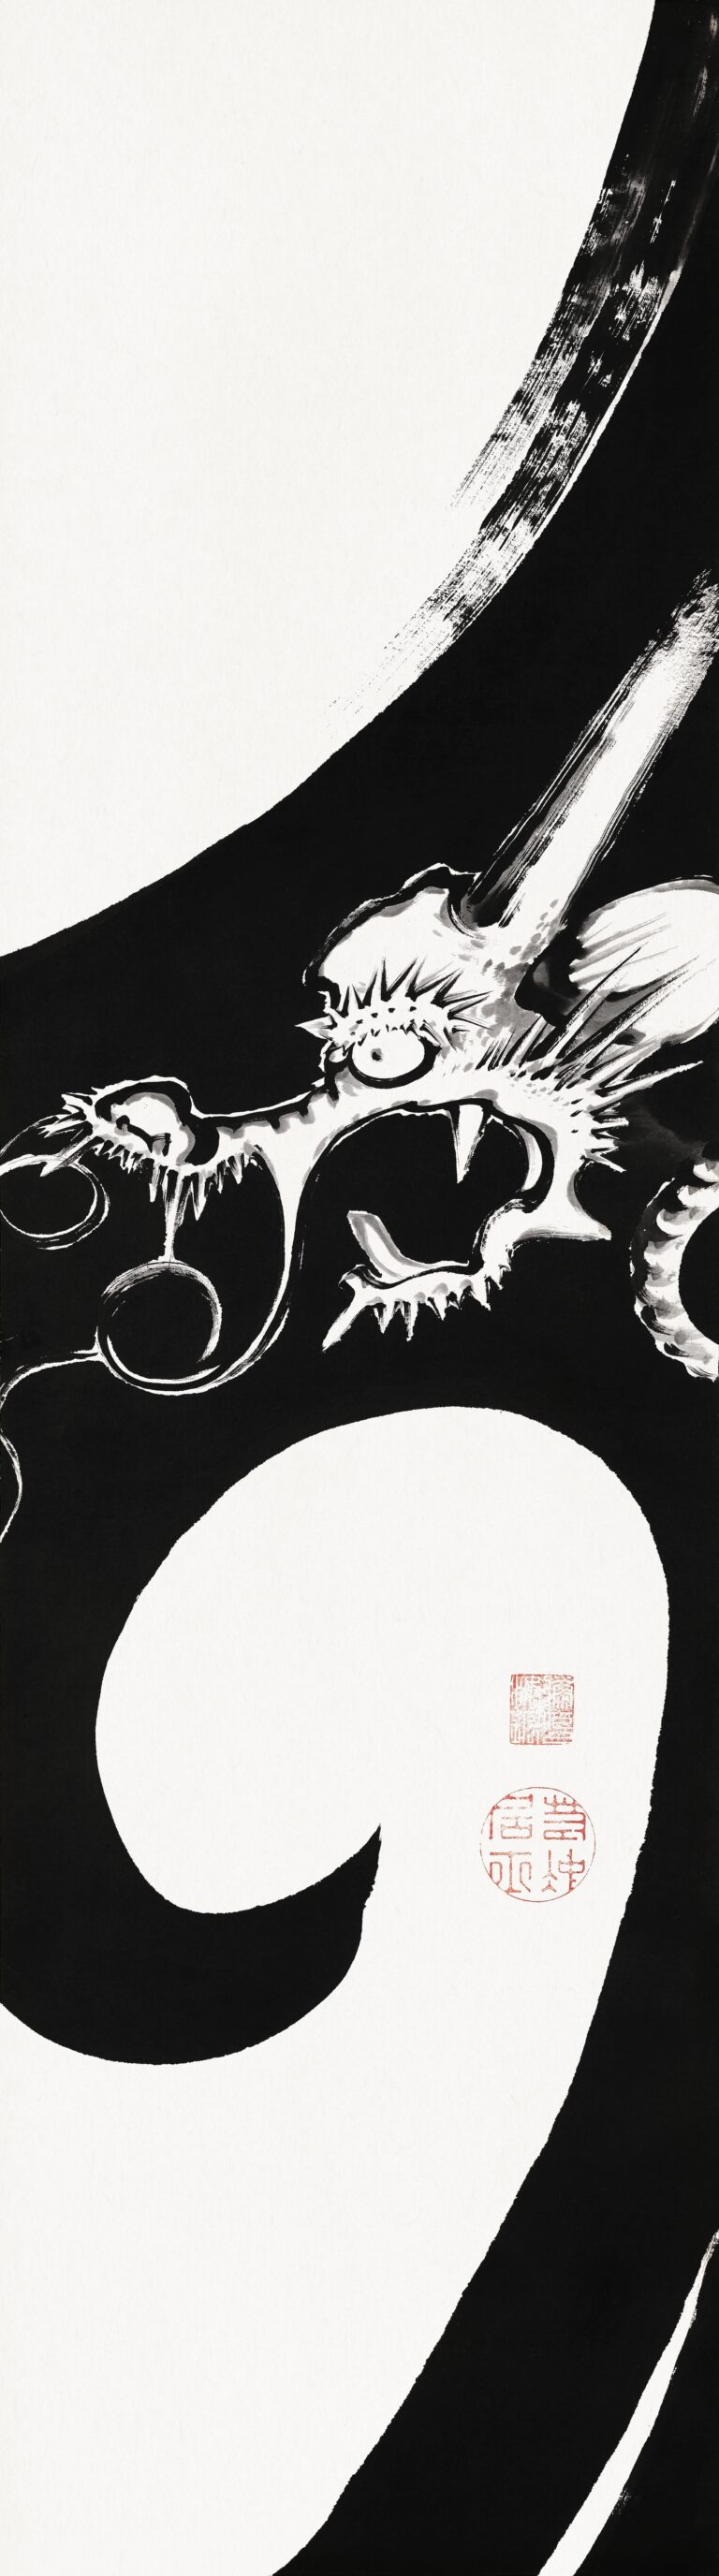
\includegraphics{../img/image02.jpg}\\

\textbf{Confía en la naturaleza original.\\
Confía en lo que ya eres.}

El \emph{Xin Xin Ming}, atribuido al Tercer Patriarca del budismo Chan,
Jianzhi Sengcan, es uno de los textos más antiguos y esenciales de la
tradición zen. A través de versos breves y profundos, señala
directamente la realidad no-dual de nuestra existencia y nos invita a
abandonar toda división entre nosotros/as y el mundo.

En este libro, Daizan Soriano ofrece una traducción cuidada y
comentarios que brotan de su práctica viva del budismo Soto Zen. Cada
poema es presentado como una puerta independiente hacia la comprensión
inmediata, permitiendo al lector o lectora adentrarse en el corazón de
la enseñanza desde cualquier página.

\textbf{Explora cómo soltar toda búsqueda y reconocer, aquí y ahora, la
plenitud de la naturaleza original.}

\end{document}
